\chapter{Implementación del sistema}
%
\section{Implementación de los drones}
Para el proceso de documentación del armado de los drones, se tiene en cuenta los siguientes elementos : 
\begin{itemize}[itemsep=0pt,parsep=0pt,topsep=0pt,partopsep=0pt]
  \item Chasis de Kit: S500
  \item Propelas: Nylon 1045
  \item Motor sin escobillas: 2212 920KV
  \item Controladoras de Velocidad: RC Brushless (ESC)
  \item Power Distribution Board (PDB) y Power Module: Apm2.8 2.6 2.52
  \item Batería LiPo 3S de 11.1V - 5000mAh
  \item Controladora de vuelo: Pixhawk 2.4.8
  \item Sistema de GPS: HERE+
  \item Sistema de Telemetría NRF24L01
  \item Transceptor De Telemetría Personalizado: NRF24L01
  \item RaspBerry Pi4
  \item Xiangtat Flysky FS-i6X 2.4GHz 10CH AFHDS 2A RC Transmisor TX con receptor iA6B (Radio transmisor para control manual)
\end{itemize}

\noindent Comenzando con el armado del dron, se utilizará el Chasis S500, el cual viene con los siguientes elementos:
\begin{itemize}[itemsep=3pt,parsep=0pt,topsep=0pt,partopsep=0pt]
  \item Placa central PCB con punto de soldadura
  \item Tubos de fibra de carbono de 16 mm de diámetro con una altura de 250 mm
  \item Tubos de fibra de carbono de 10 mm de diámetro con longitud de 250 mm para la base
  \item Tubos de esponja anti salto
  \item Brazos DJI S800 EVO con 6 agujeros para colocar motores
\end{itemize}
\begin{figure}[H]
    \centering
    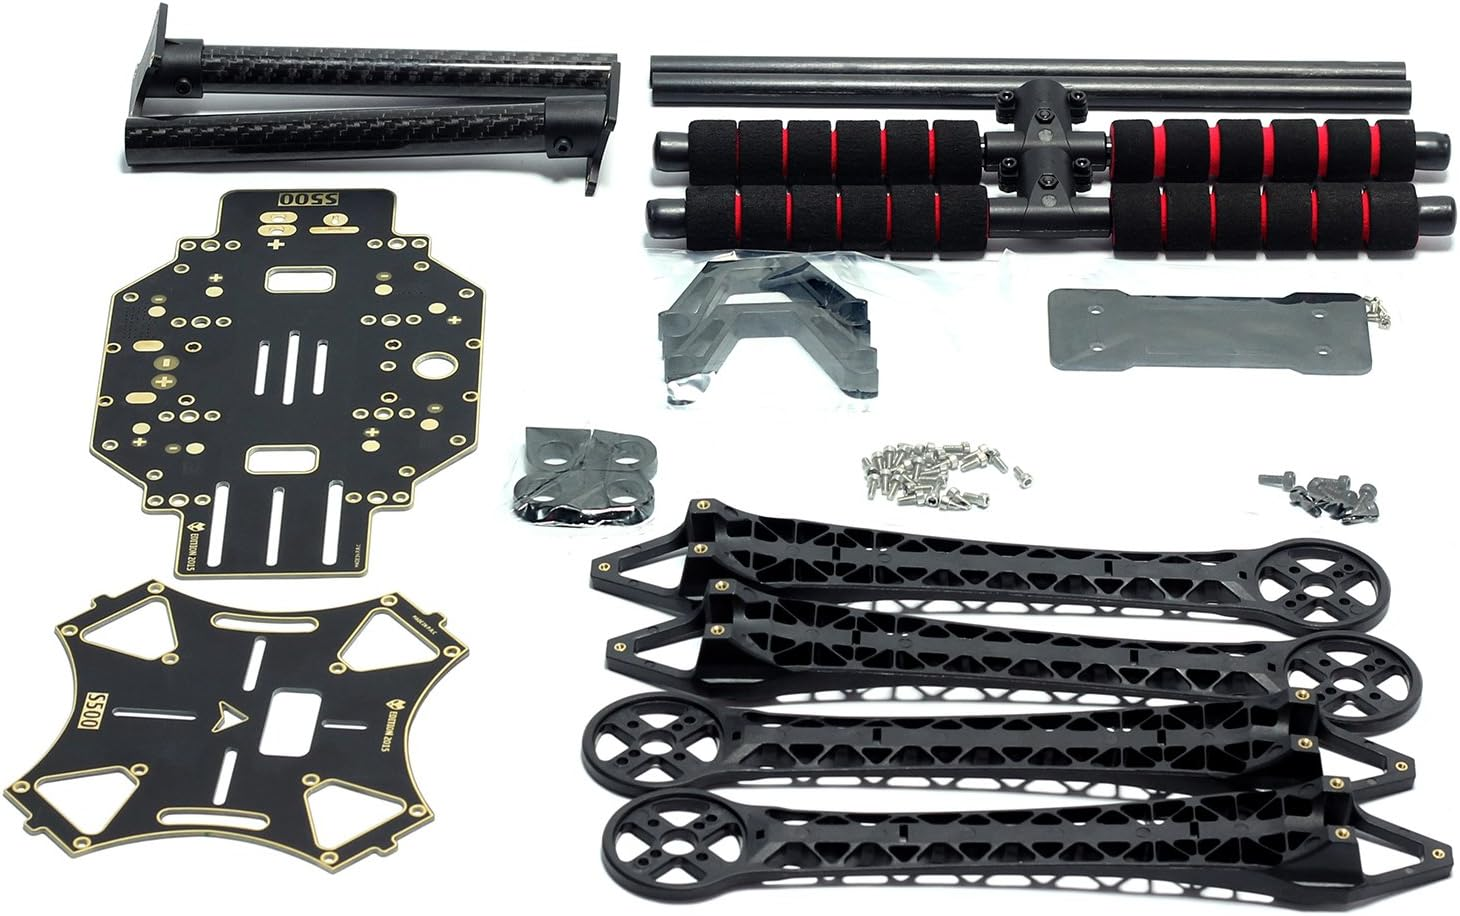
\includegraphics[width=0.6\textwidth]{imagenes/componenteskit.png}
    \caption{Componentes del Kit S500.}
    \label{fig:kitS500}
\end{figure}
El primer paso para el armado del chasis S500 es para el tren de aterrizaje. Se arma tal como se muestra en la siguiente imagen:
\begin{figure}[H]
    \centering
    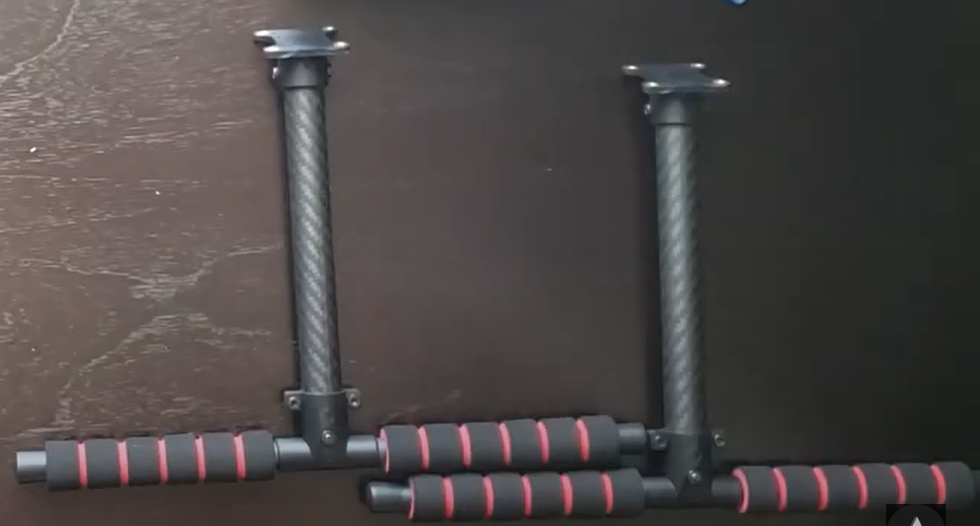
\includegraphics[width=0.7\textwidth]{imagenes/base-tren.png}
    \caption{Base para el tren de aterrizaje.}
    \label{fig:basetren}
\end{figure}

\noindent Se colocan los tubos de fibra de carbono para que formen la base del cuadricóptero. Se van a montar sobre la placa central para formar la base.
\begin{figure}[H]
    \centering
    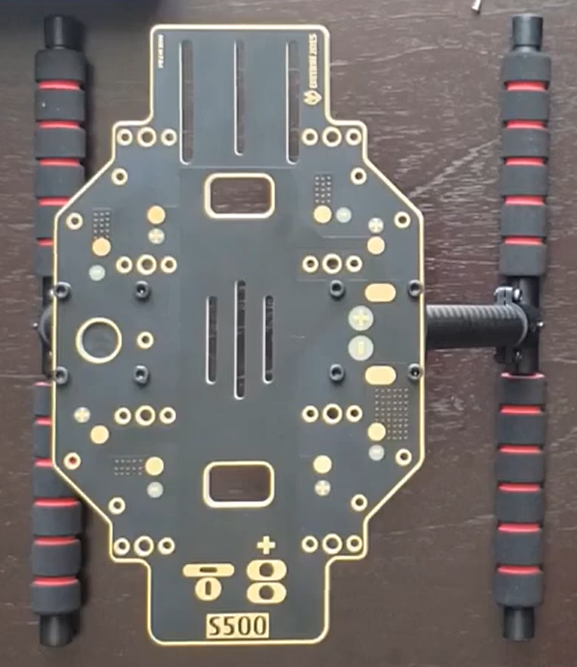
\includegraphics[width=0.45\textwidth]{imagenes/chasis-sobre-tren.png}
    \caption{Chasis montado sobre el tren de aterrizaje.}
    \label{fig:basetren}
\end{figure}
\noindent Cuando ya está la base armada, se procede al armado de los brazos de la placa superior que consta de los 4 brazos y la placa superior.

\begin{figure}[H]
    \centering
   {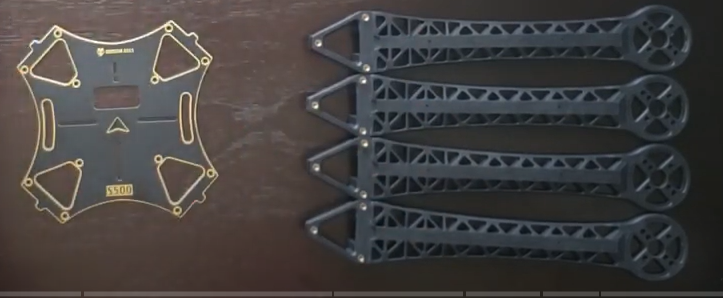
\includegraphics[width=0.7\textwidth]{imagenes/brazos.png}} 
    {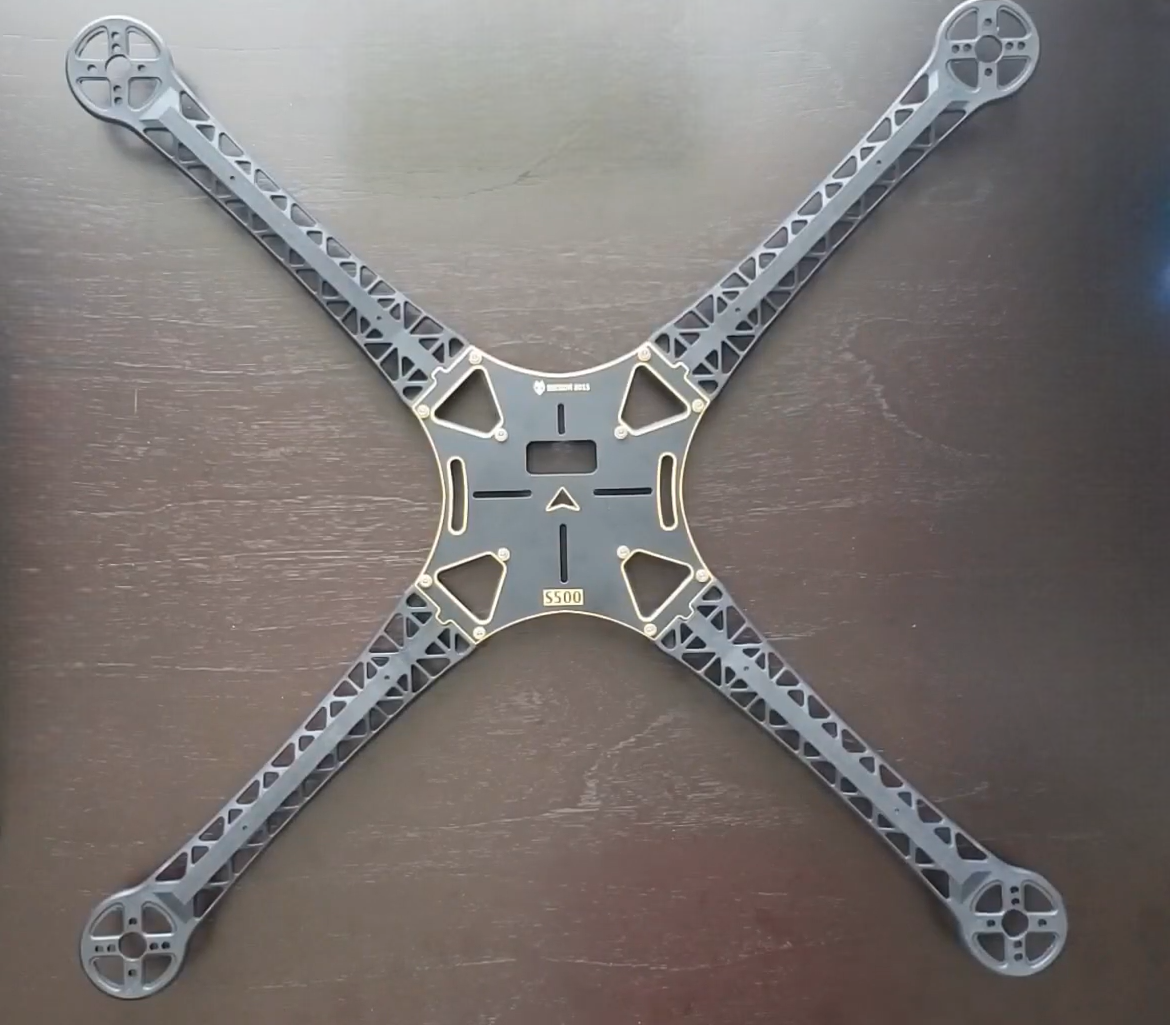
\includegraphics[width=0.7\linewidth]{imagenes/brazos-armados.png}}
    \caption{Base con 4 brazos para el armado de la placa superior.}
    \label{fig:lora-solo}
\end{figure}

\noindent Cuando la placa superior esté armada, se colocan los controladores de velocidad (ESC), los cuales debe tener en cuenta el sentido de giro de los motores y el diseño de las propelas como se muestra en la siguiente figura:

\begin{figure}[H]
    \centering
    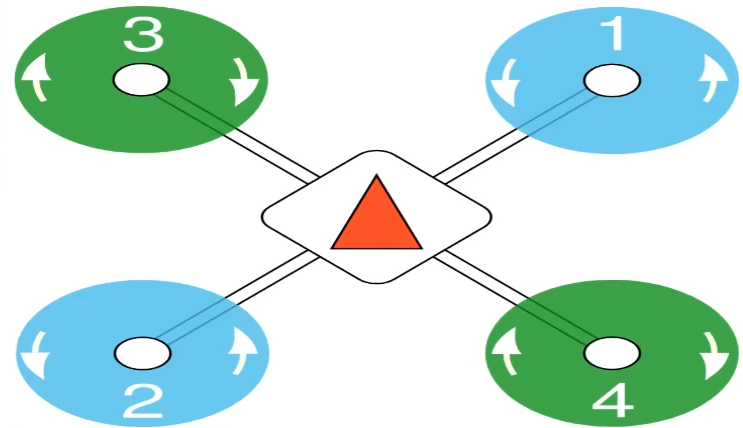
\includegraphics[width=0.5\textwidth]{imagenes/sentidodegiro.png}
    \caption{Sentido de giro de los motores.}
    \label{fig:basetren}
\end{figure}
\noindent Con esta consideración en los extremos se soldan los controladores de velocidad ESC con el tablero de distribución de energía (PDB) y el módulo de potencia.. El amperaje del ESC depende de la corriente que consumen los motores, siendo de 20\% más amperaje cómo mínimo (si el motor consume 10A, el ESC debe ser de 12A como mínimo).
\begin{figure}[H]
    \centering
    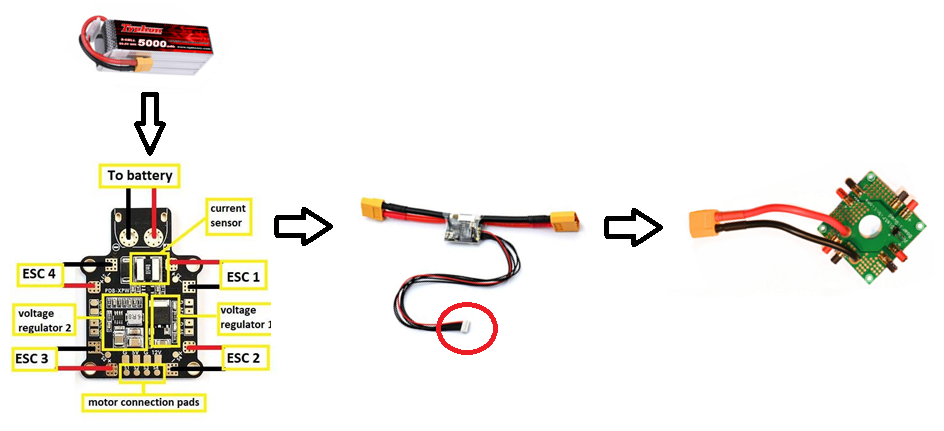
\includegraphics[width=\textwidth]{imagenes/componentes-potencia.png}
    \caption{Componentes de la parte de potencia del dron.}
    \label{fig:basetren}
\end{figure}
\newpage
\begin{figure}[H]
    \centering
    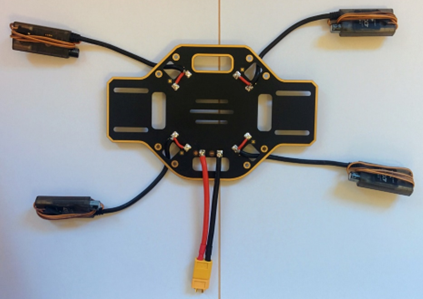
\includegraphics[width=0.7\textwidth, height=7cm]{imagenes/placa-esc.png}
    \caption{Placa superior con las ESC montadas y sin brazos.}
    \label{fig:basetren}
\end{figure}
\noindent Una vez teniendo el conjunto de las ESC y los módulos de distribución de potencia soldados, se procede a instalar los motores. Los motores utilizados son los motores sin escobillas: 2212 920KV que cuentan con las siguientes características.
\begin{itemize}
    \item Eficiencia máxima: 80\%
    \item Eficiencia de la corriente máxima: 4-10A ($>$ 75\%)
    \item Capacidad de corriente: 12A/60s
    \item Consumo de corriente sin carga a 10 V: 0.5A
    \item Eficiencia -MAX real: 4-10A ($>$ 75\%)
    \item RPM/V: 930 KV
    \item Diámetro del eje: 3.17mm
    \item Dimensiones: 28 x 28 x 39 mm
    \item Peso: 67g
\end{itemize}
\newpage
\begin{figure}[H]
    \centering
    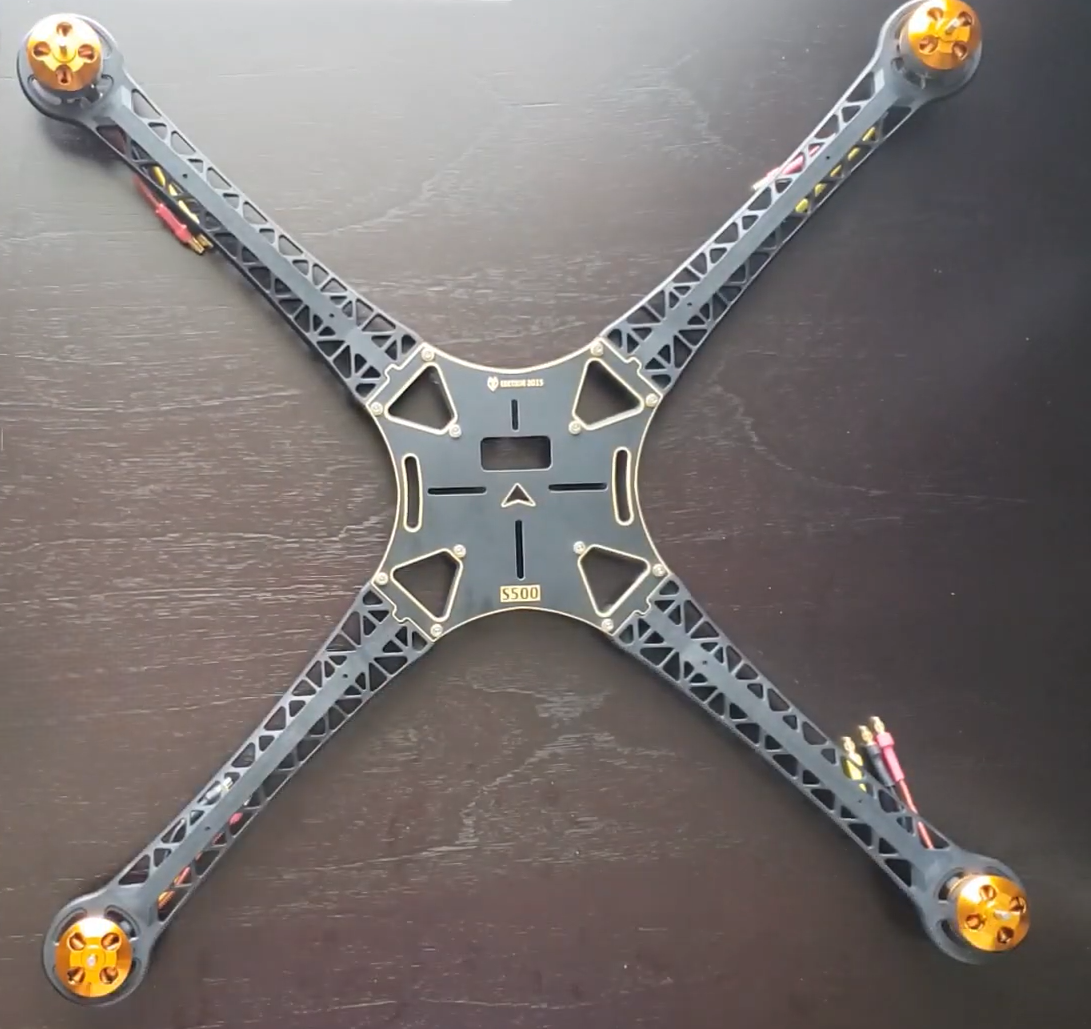
\includegraphics[width=0.5\textwidth]{imagenes/placa-motores.png}
    \caption{Placa superior con los motores montados.}
    \label{fig:basetren}
\end{figure}
\noindent Una vez ensambladas los componentes de ambas partes (la placa principal y la placa superior), únicamente hay que unir estos 2 conjuntos. Colocando la placa superior sobre la placa principal, utilizando los tornillos que ya vienen incluidos sobre el KIT S500. No hay que perder en cuenta las conexiones que se consideraron del sentido de rotación de los motores.
\begin{figure}[H]
    \centering
    {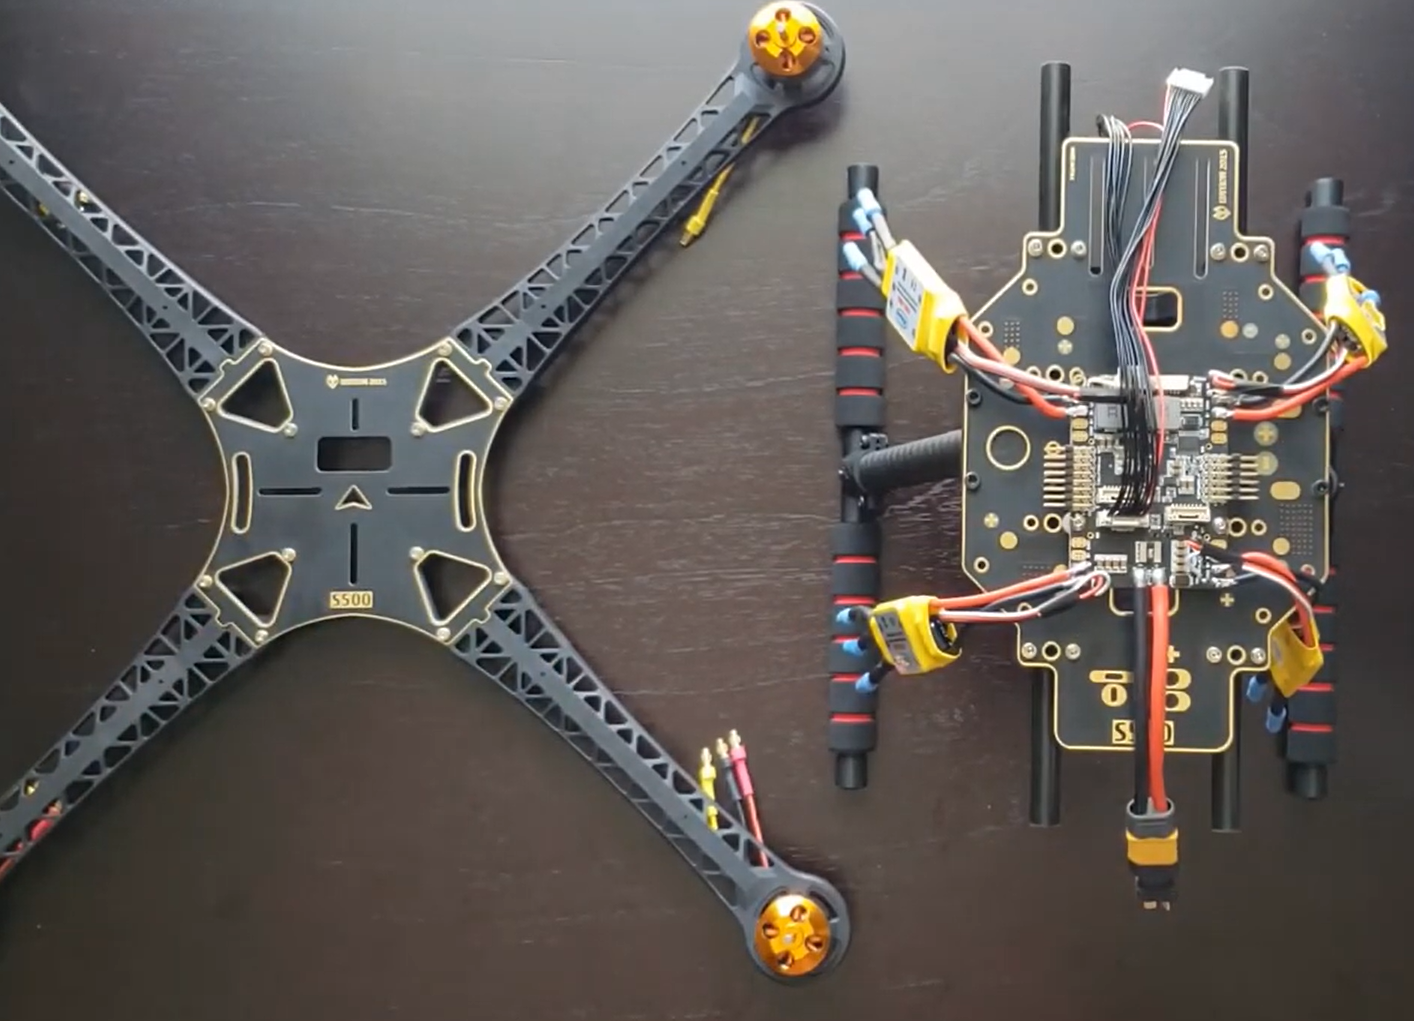
\includegraphics[width=0.5\linewidth]{imagenes/superior-inferior.png}}
    \caption{Montaje de la placa superior sobre la placa base (por partes).}
    \label{fig:lora-solo-parte1}
\end{figure}

\begin{figure}[H]
    \centering
    {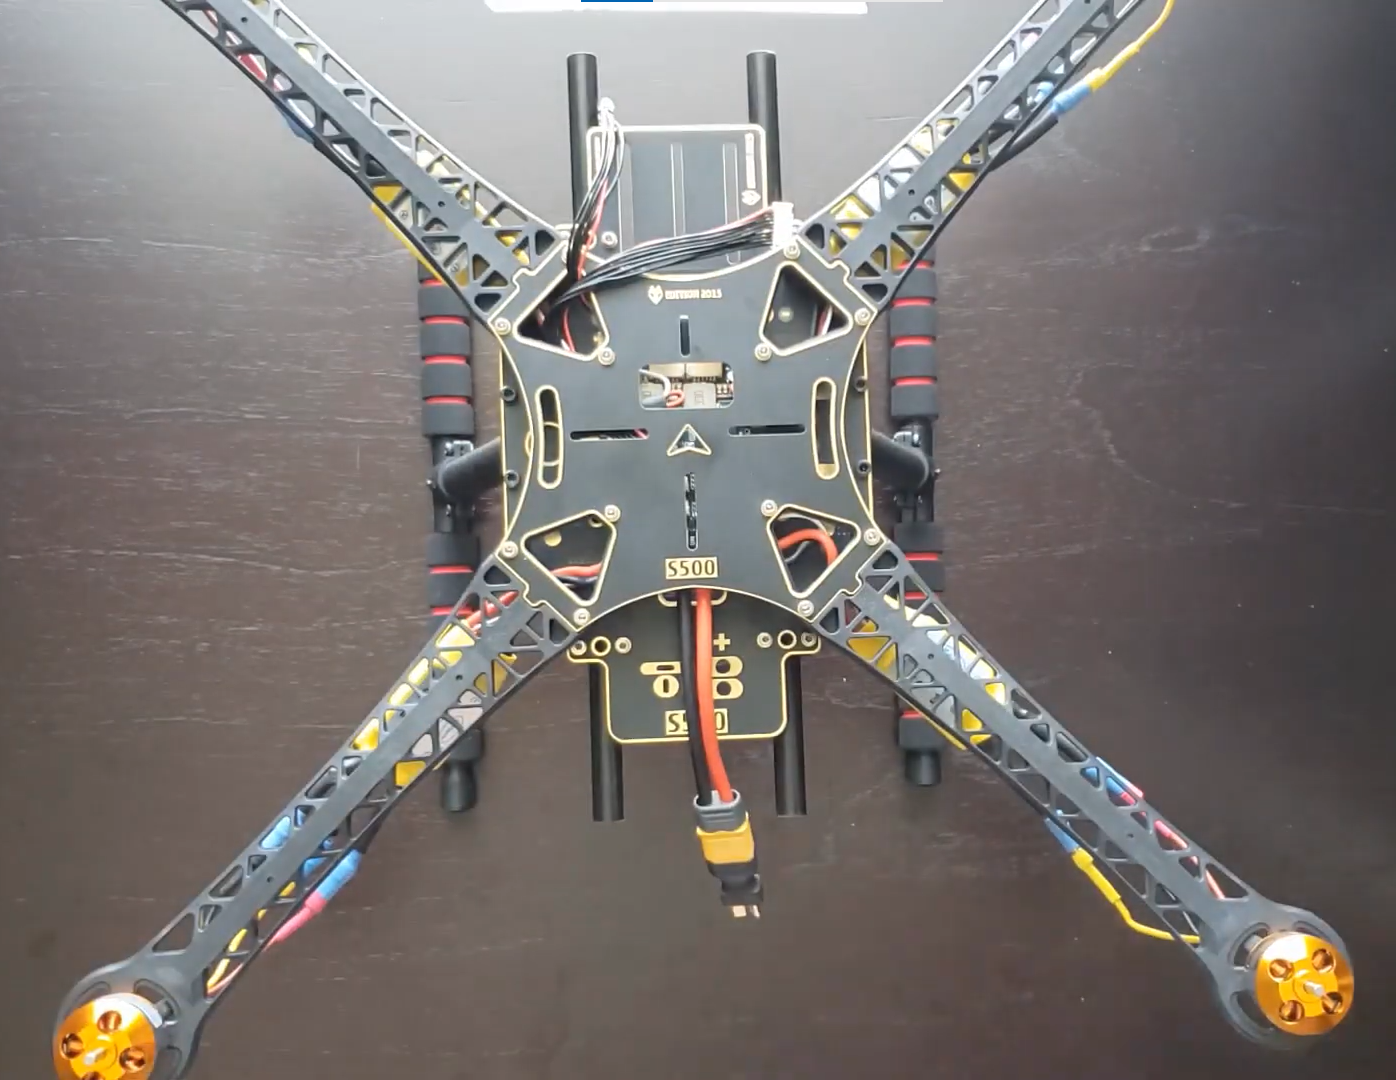
\includegraphics[width=0.5\linewidth]{imagenes/sup-inf-unidas.png}}
    \caption{Montaje de la placa superior sobre la placa base (armada).}
    \label{fig:lora-solo-parte2}
\end{figure}
\noindent Para finalizar el ensamblado básico del dron, se añade la computadora de vuelo Pixhawk 2.4.8 y el módulo GPS para el posicionamiento del dron.
Para el módulo GPS, debe estar separado mínimo 15 cm de la computadora de vuelo para no causar interferencia, por lo que se le coloca en un mástil que irá en la parte superior.
\begin{figure}[H]
    \centering
    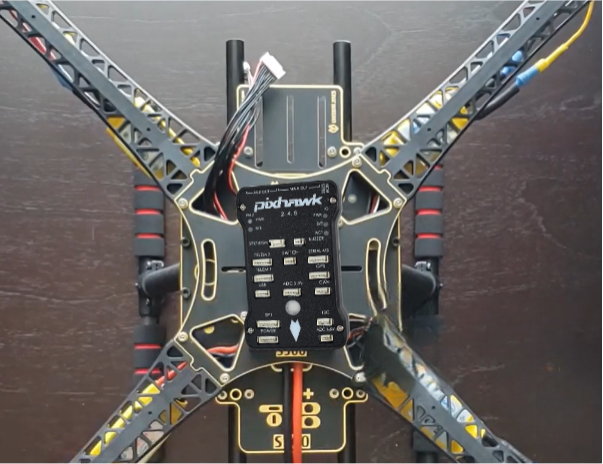
\includegraphics[width=0.5\textwidth]{imagenes/pix-montada.png}
    \caption{Montaje de la computadora de vuelo sobre la placa superior.}
\end{figure}
\begin{figure}[H]
    \begin{minipage}{\textwidth}
        \centering
        \begin{minipage}{\textwidth}
            \centering
            \subfigure[) Individualmente.]{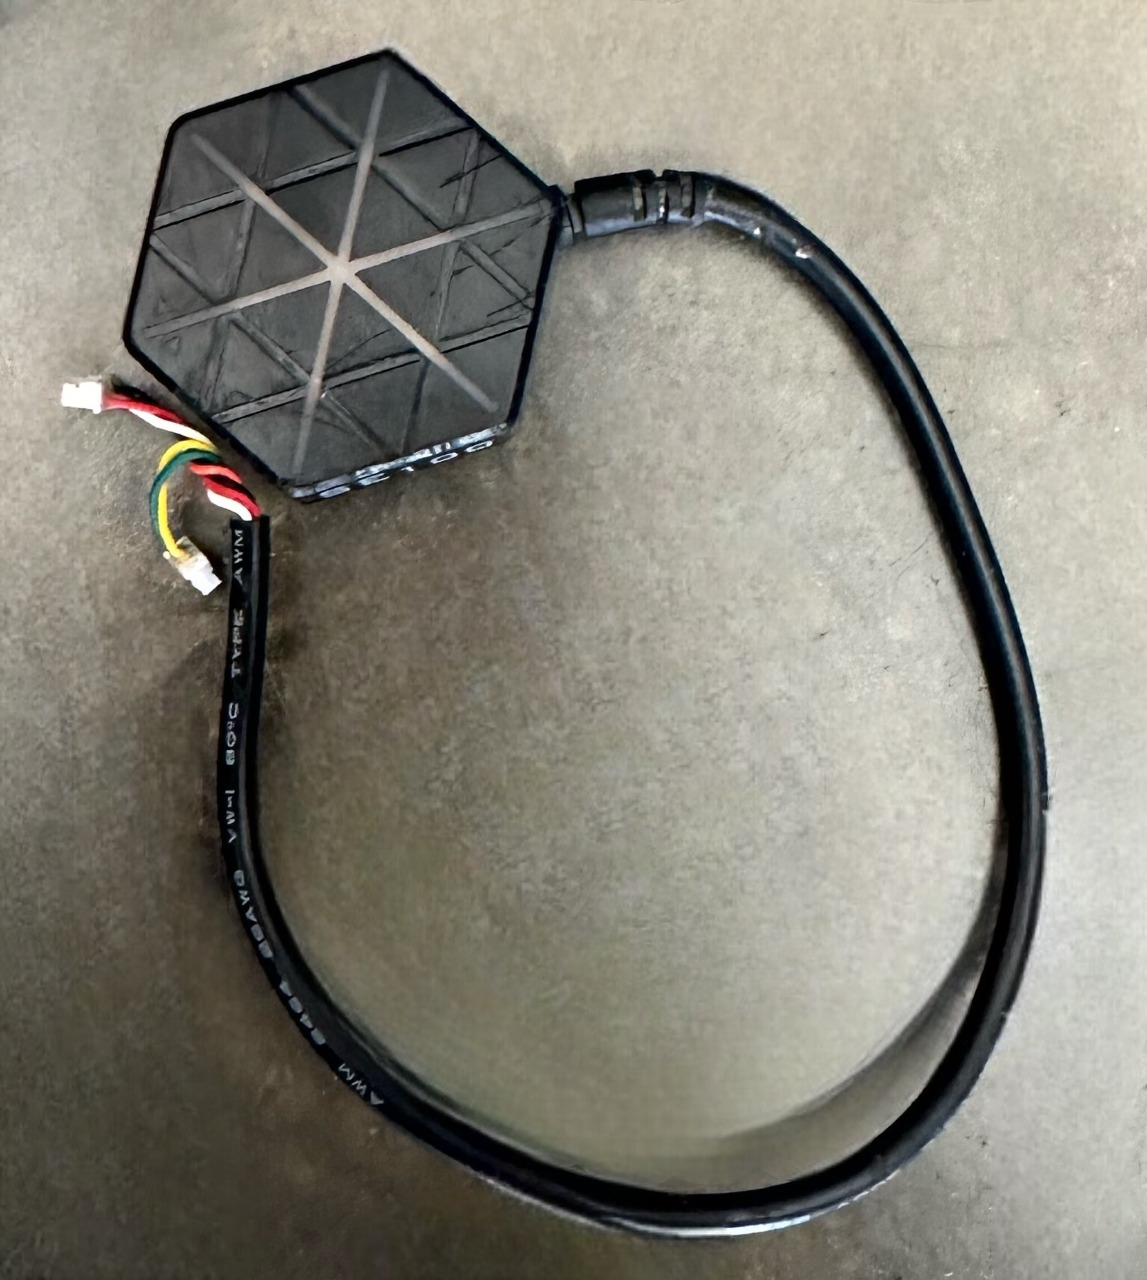
\includegraphics[width=0.3\textwidth]{imagenes/gps-sindron.jpeg}}\hspace{0.1\textwidth}
            \subfigure[) Mástil.]{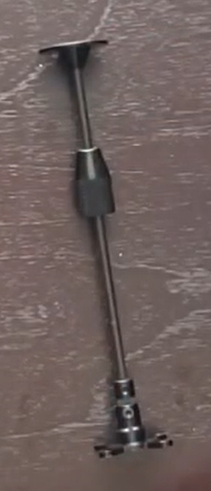
\includegraphics[width=0.15\textwidth]{imagenes/mastil.png}}
        \end{minipage}
    \end{minipage}
    
    \begin{minipage}{\textwidth}
        \centering
        \begin{minipage}{\textwidth}
            \centering
            \subfigure[)  Montado.]{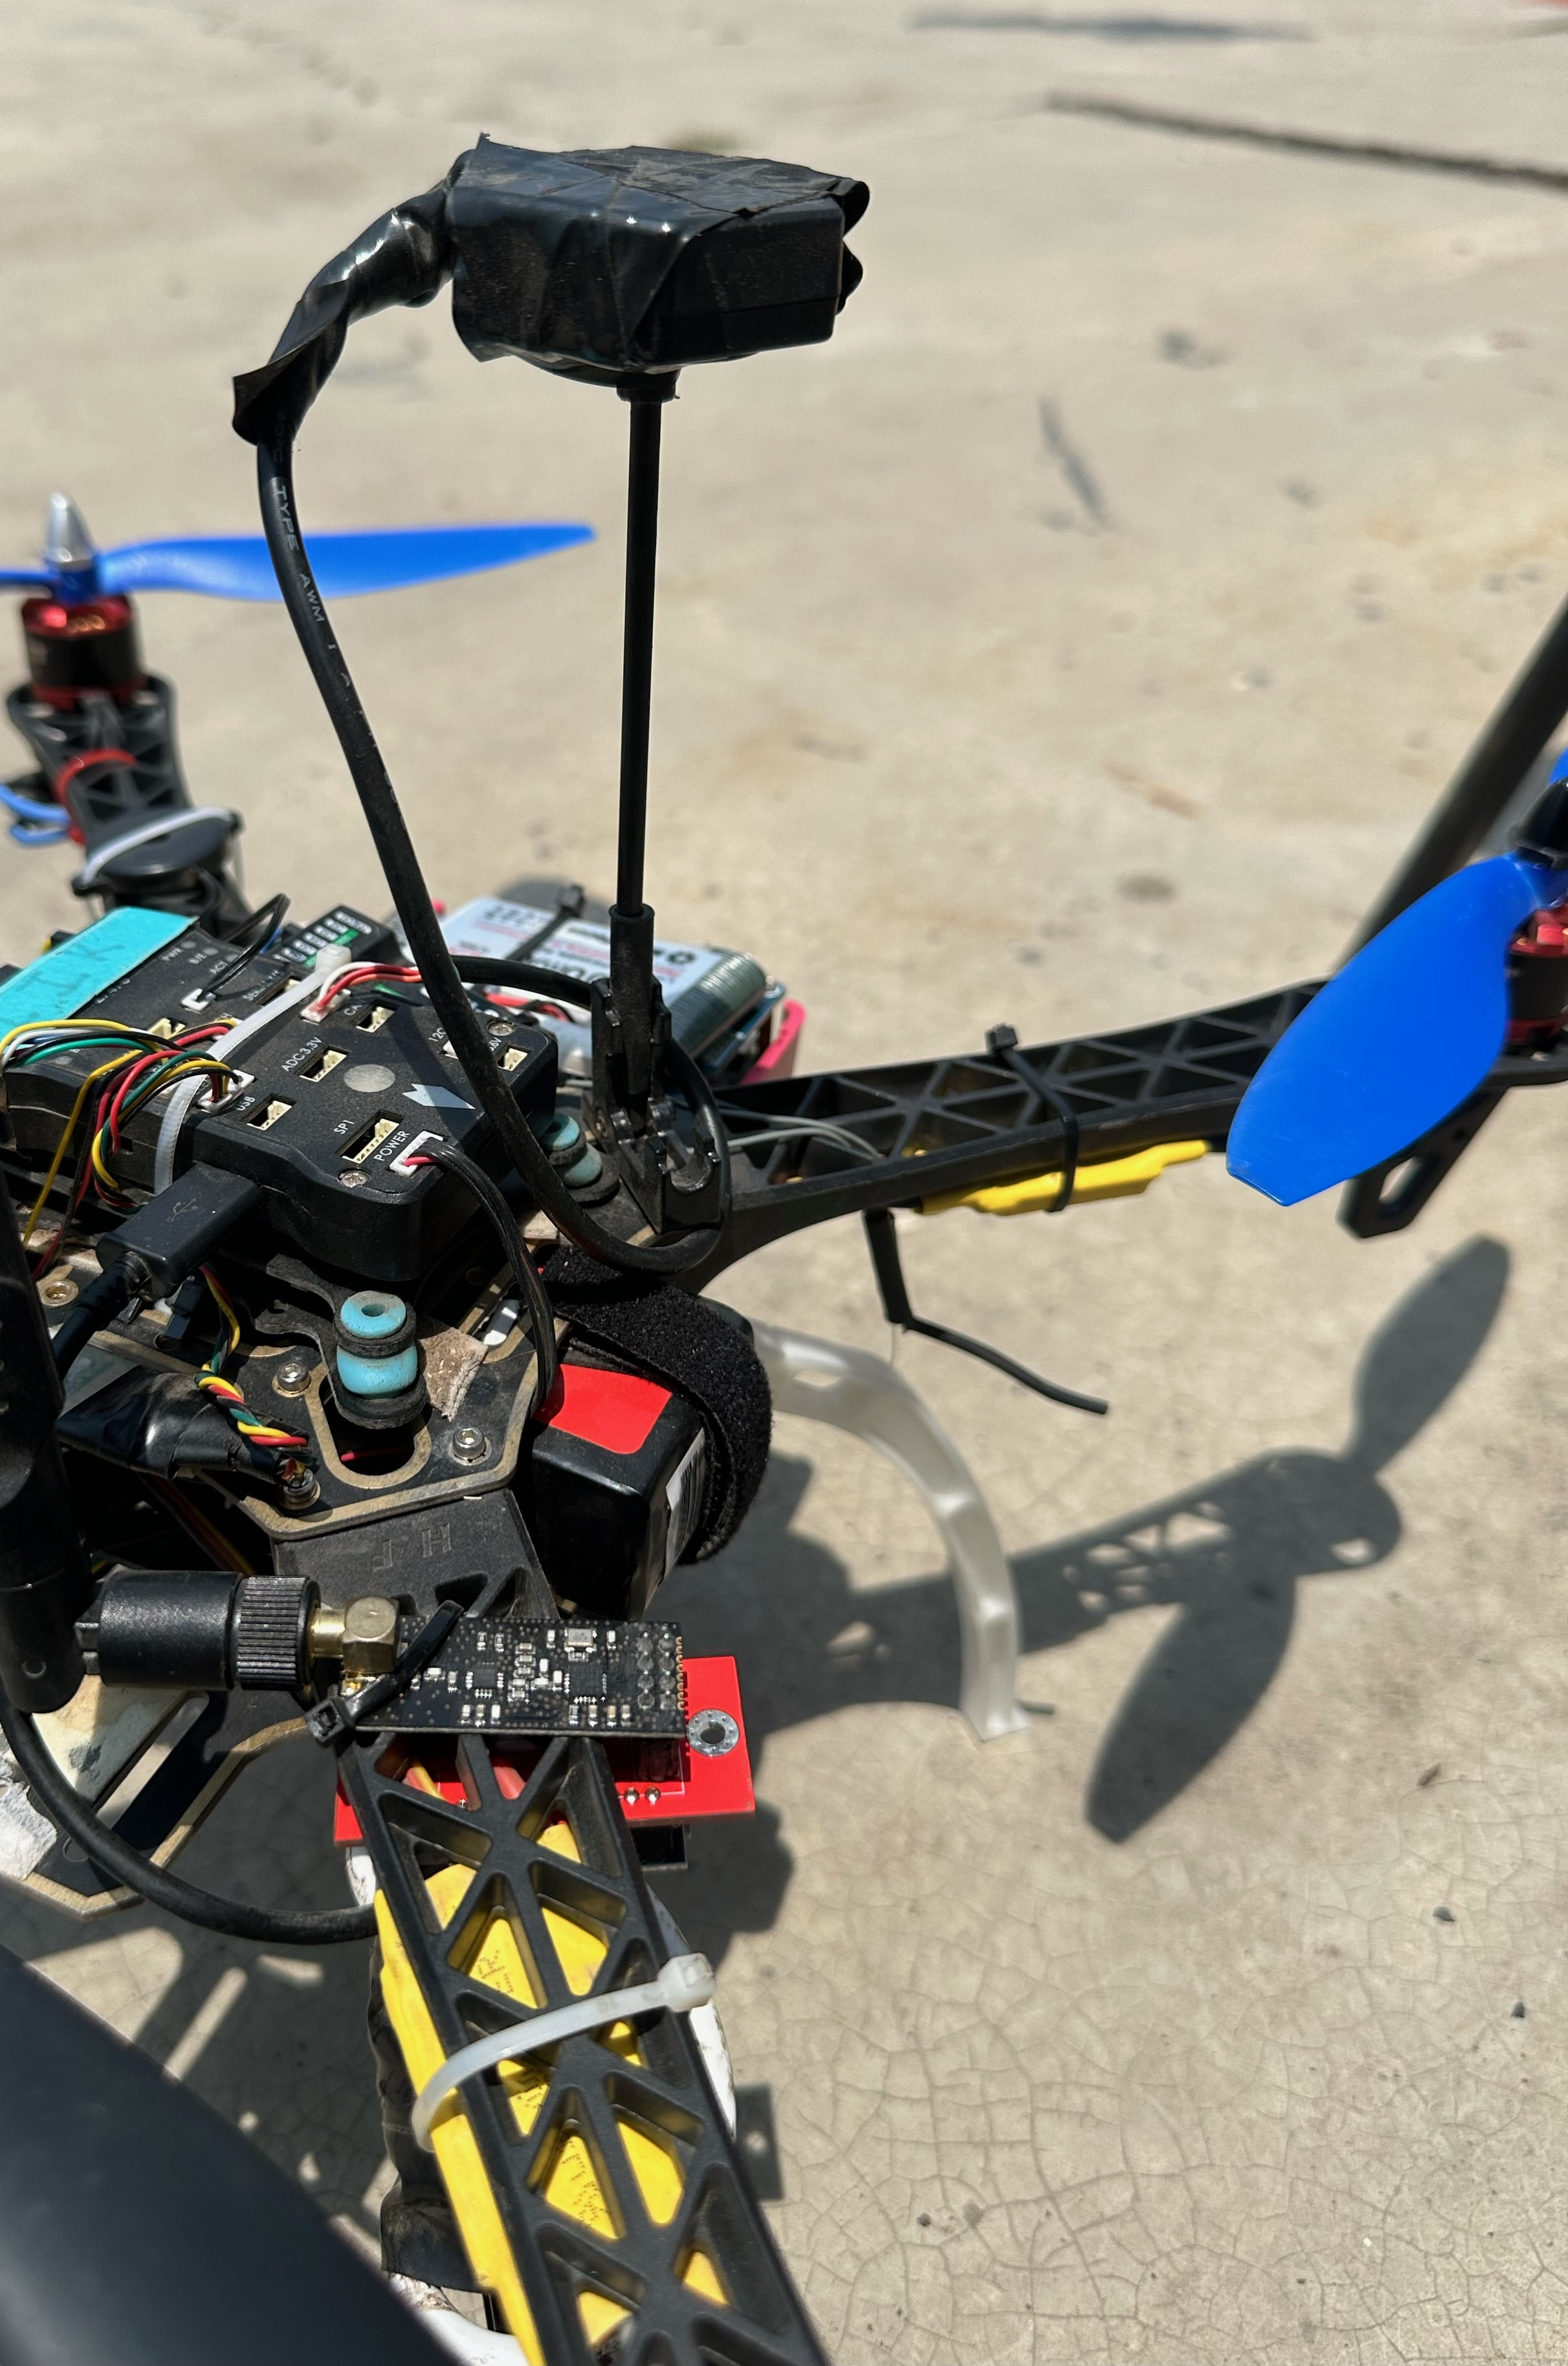
\includegraphics[width=0.35\textwidth]{imagenes/gps-montado.jpeg}}
        \end{minipage}
    \end{minipage}
    
    \caption{Montaje del GPS de vuelo sobre la placa superior.}
\end{figure}

La computadora de vuelo Pixhawk 2.4.8 cuenta con las siguientes características:
\begin{itemize}[itemsep=0pt, parsep=0pt, topsep=0pt]
    \item \textbf{Microprocesador}
    \begin{itemize}[label=o, itemsep=0pt, parsep=0pt, topsep=0pt, partopsep=0pt]
        \item Frecuencia: 168 MHZ, 256K RAM
        \item Coprocesador de copia de seguridad 32 STM32F103
    \end{itemize}
    \item \textbf{Sensor}
    \begin{itemize}[label=o, itemsep=0pt, parsep=0pt, topsep=0pt, partopsep=0pt]
        \item Giroscopio digital de 3 ejes L3GD20 16
        \item Acelerómetro de 3 ejes LSM303D 14/Magnetómetro
        \item Acelerómetro / magnetómetro MPU6000 de 6 ejes
        \item Barómetro de precisión MS5607
    \end{itemize}
    \item \textbf{Interfaz}
    \begin{itemize}[label=o, itemsep=0pt, parsep=0pt, topsep=0pt, partopsep=0pt]
        \item UART 1, 2 compatible con alto voltaje con control de flujo de hardware
        \item Entrada compatible con receptor de satélite Spektrum DSM / DSM2 / DSM-X
        \item Entradas y salidas compatibles con Futaba SBUS
        \item Entrada de señal PPM
        \item Entrada RSSI (PWM o voltaje) 
        \item I2C 
        \item SPI 
        \item 3.3 y entrada 6.6VADC 
        \item Interfaz micro USB externa
    \end{itemize}
\end{itemize}
\begin{figure}[H]
    \centering
    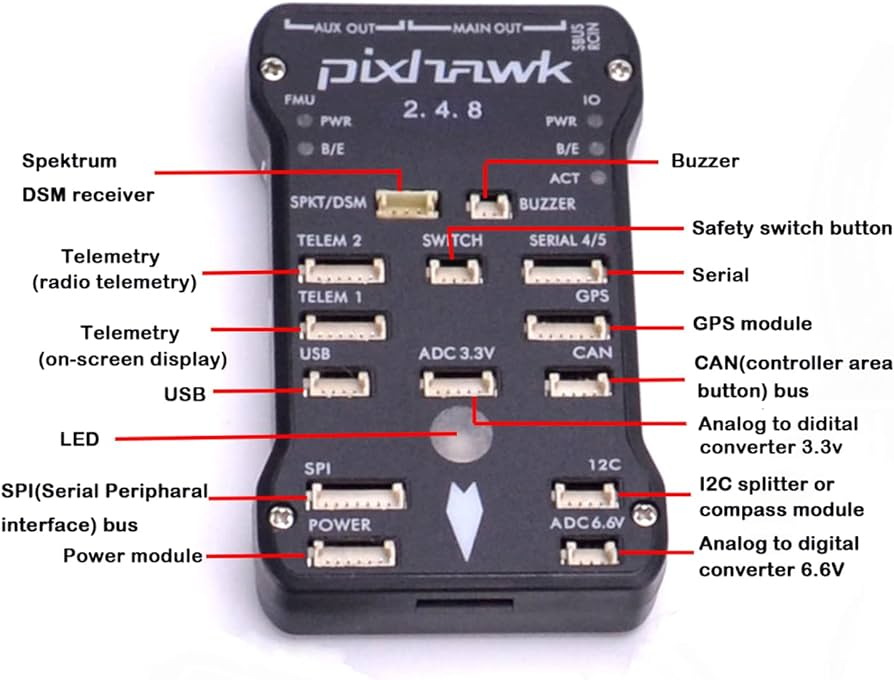
\includegraphics[width=0.6\textwidth, height=7cm]{imagenes/diagrama-pix.png}
    \caption{Diagrama de conexiones de la computadora de vuelo Pixhawk 2.4.8}
    \label{fig:basetren}
\end{figure}
\noindent Se utilizan las conexiones de POWER, las 2 de telemetría, el módulo GPS, el buzzer, el safety switch y la comunicación I2C, como se muestra en la siguiente figura:
\begin{figure}[H]
    \centering
    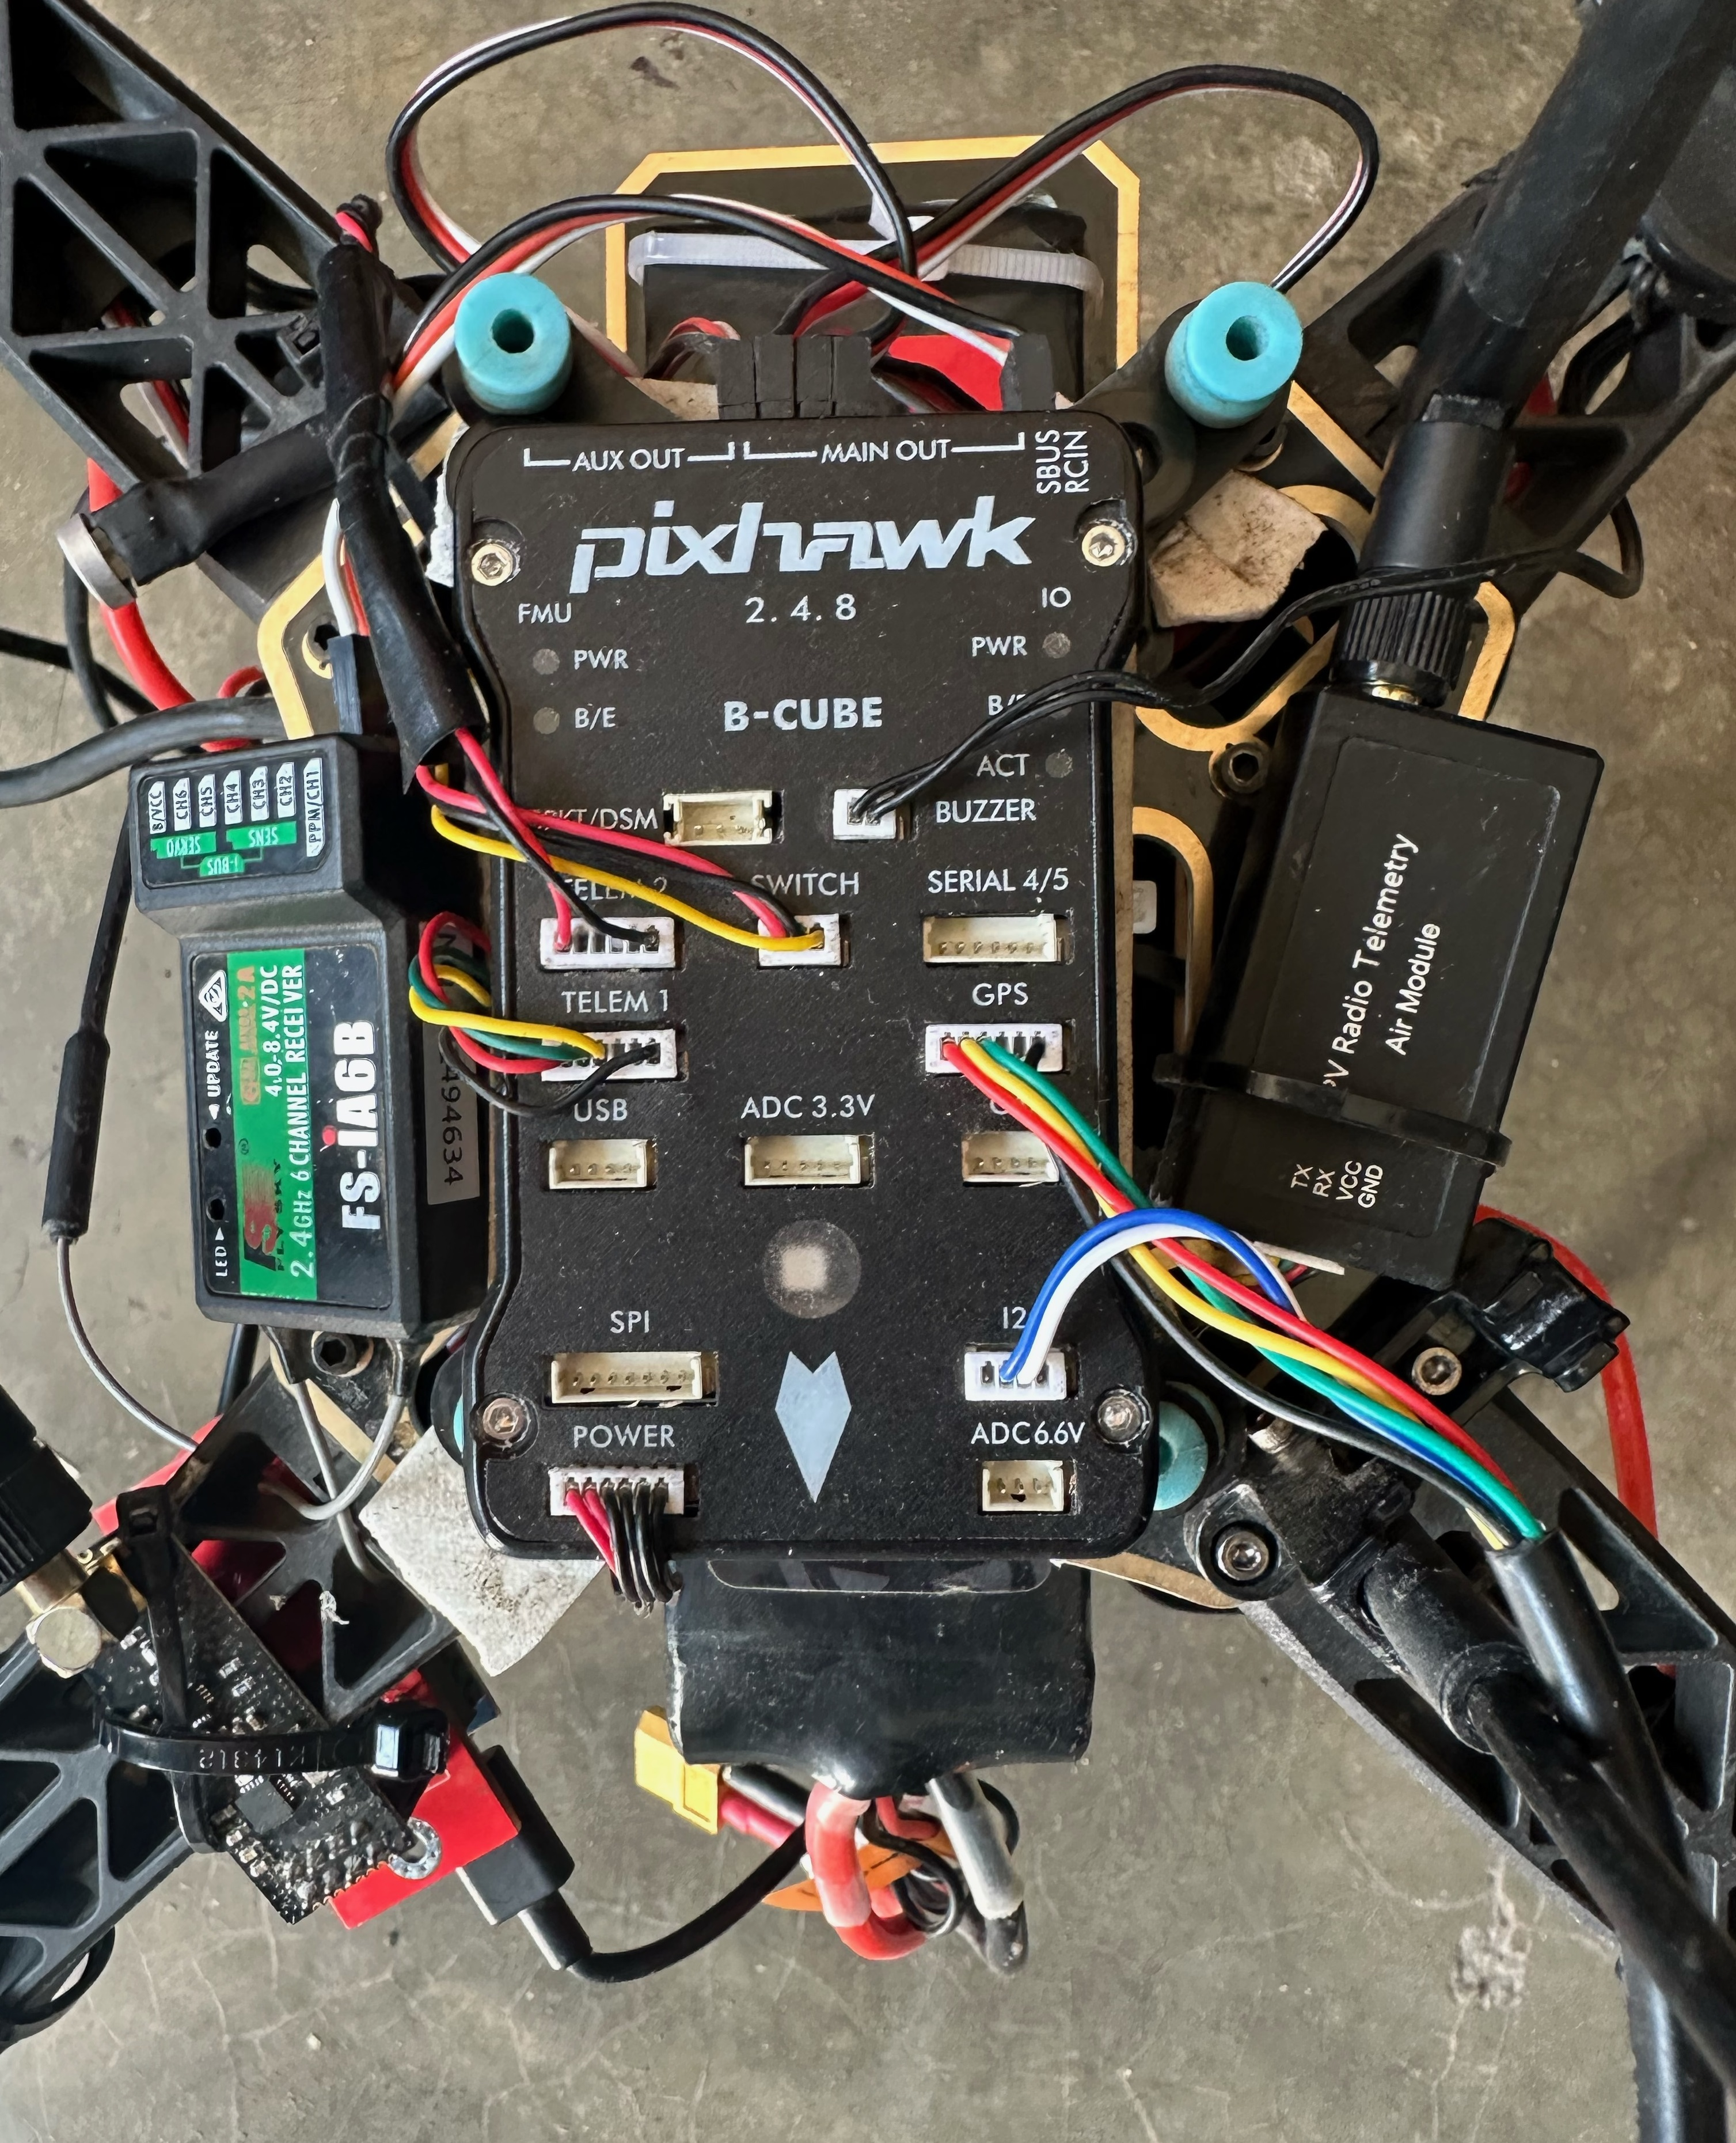
\includegraphics[width=0.5\textwidth, height=7cm]{imagenes/pix.jpeg}
    \caption{Conexiones sobre la computadora de vuelo.}
    \label{fig:basetren}
\end{figure}

\noindent Para la parte específica de control del dron, se le añade otra computadora, la Raspberry Pi4, ya que contiene las librerías para el protocolo MavLink, cuenta con los puertos suficientes para conectar dispositivos y tiene la capacidad de procesar señales digitales (DSP) en caso de ser necesario. Algunos de los usos de la Raspberry Pi 4 para este proyecto podrían incluir:
\begin{itemize}
    \item \textbf{Control de vuelo:} Puede ejecutar algoritmos de control de vuelo y software de navegación para dirigir los drones (enjambre de drones) de manera autónoma o semi-autónoma.
    \item \textbf{Interfaz de usuario y monitoreo:} Se puede utilizar Python para desarrollar una interfaz de usuario en la Raspberry Pi 4 que permita supervisar y controlar los drones de manera intuitiva.
\end{itemize}
Esta computadora externa al ser montada en el dron, se alimenta independientemente de la batería principal utilizando una batería externa.
\begin{figure}[H]
    \begin{minipage}{\textwidth}
        \centering
        \begin{minipage}{\textwidth}
            \centering
            \subfigure[) Individualmente.]{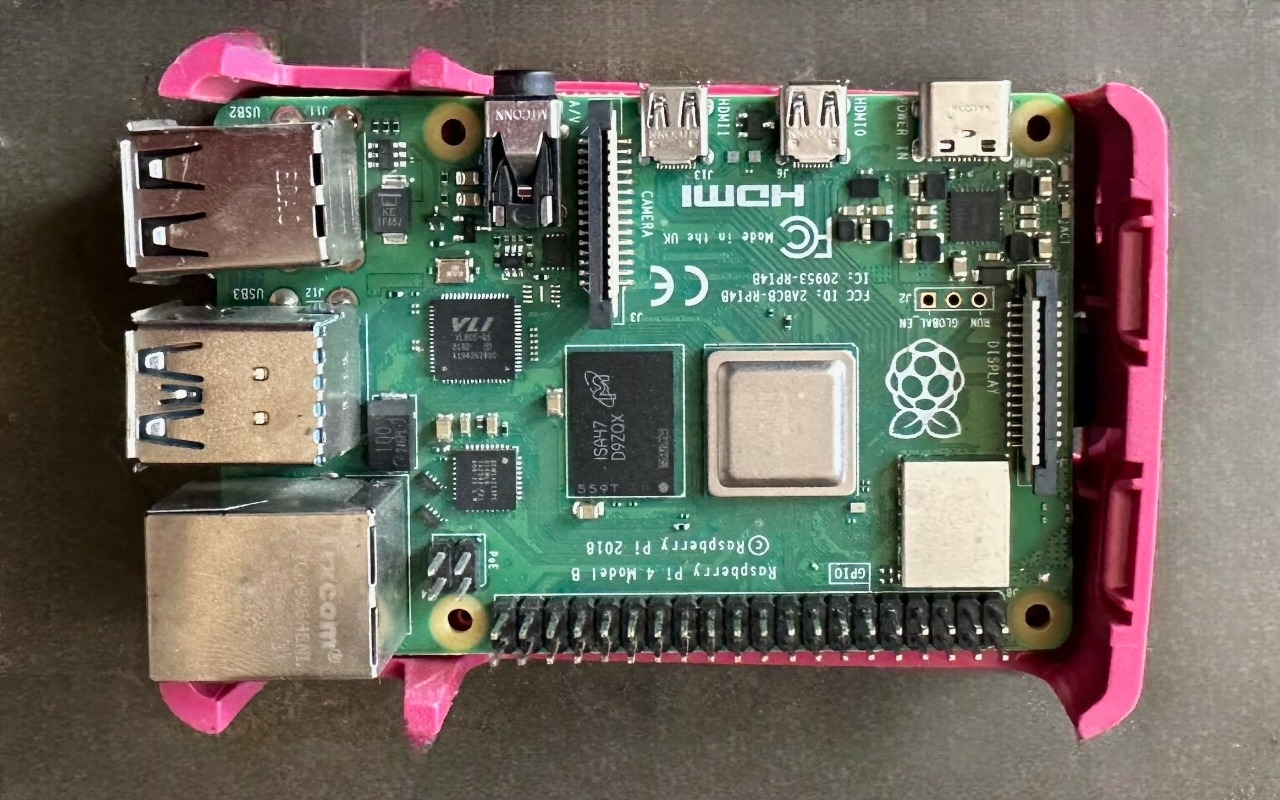
\includegraphics[width=0.45\textwidth, height=4.5cm]{imagenes/rasp.jpeg}}
            \subfigure[) Con batería de 3000mAh.]{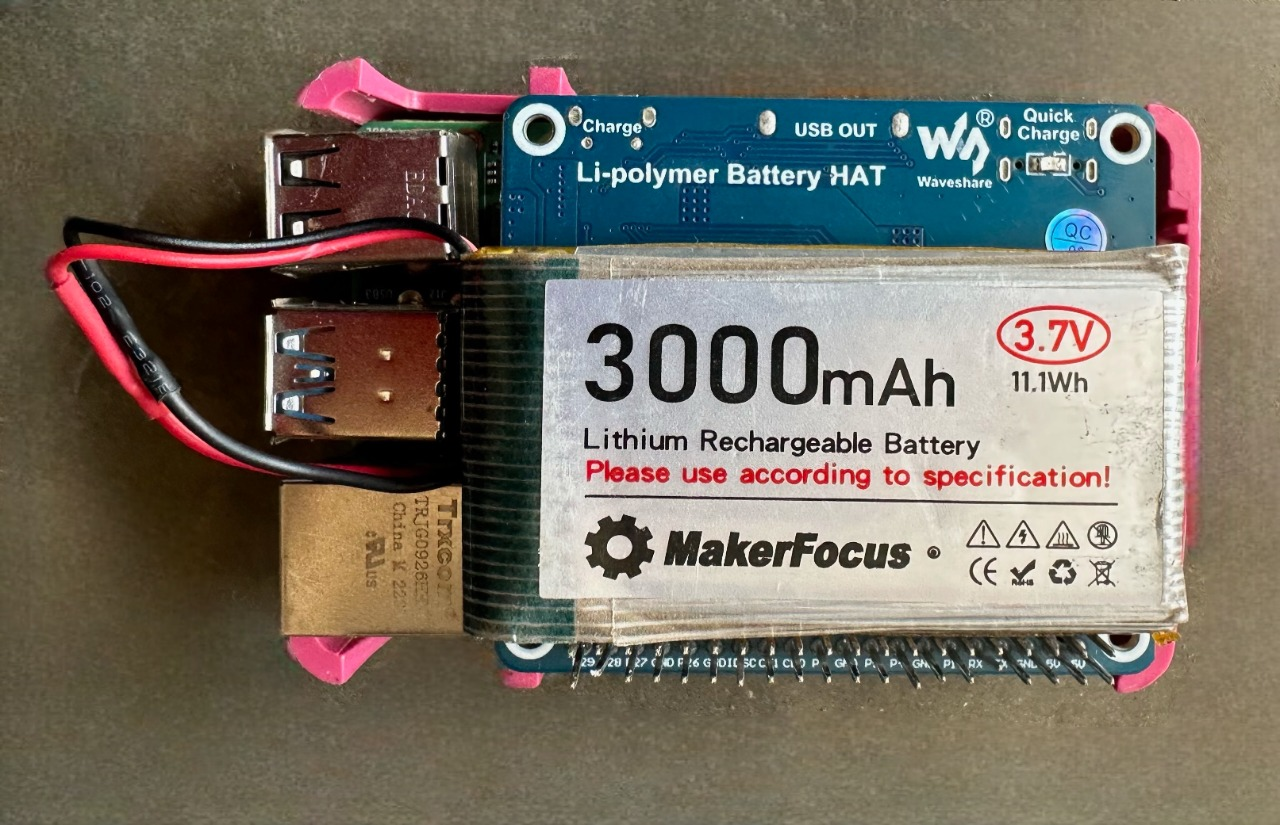
\includegraphics[width=0.45\textwidth, height=4.5cm]{imagenes/rasp-bateria.jpeg}}
        \end{minipage}
    \end{minipage}
    
    \begin{minipage}{\textwidth}
        \centering
        \begin{minipage}{\textwidth}
            \centering
            \subfigure[)  Montada con su batería.]{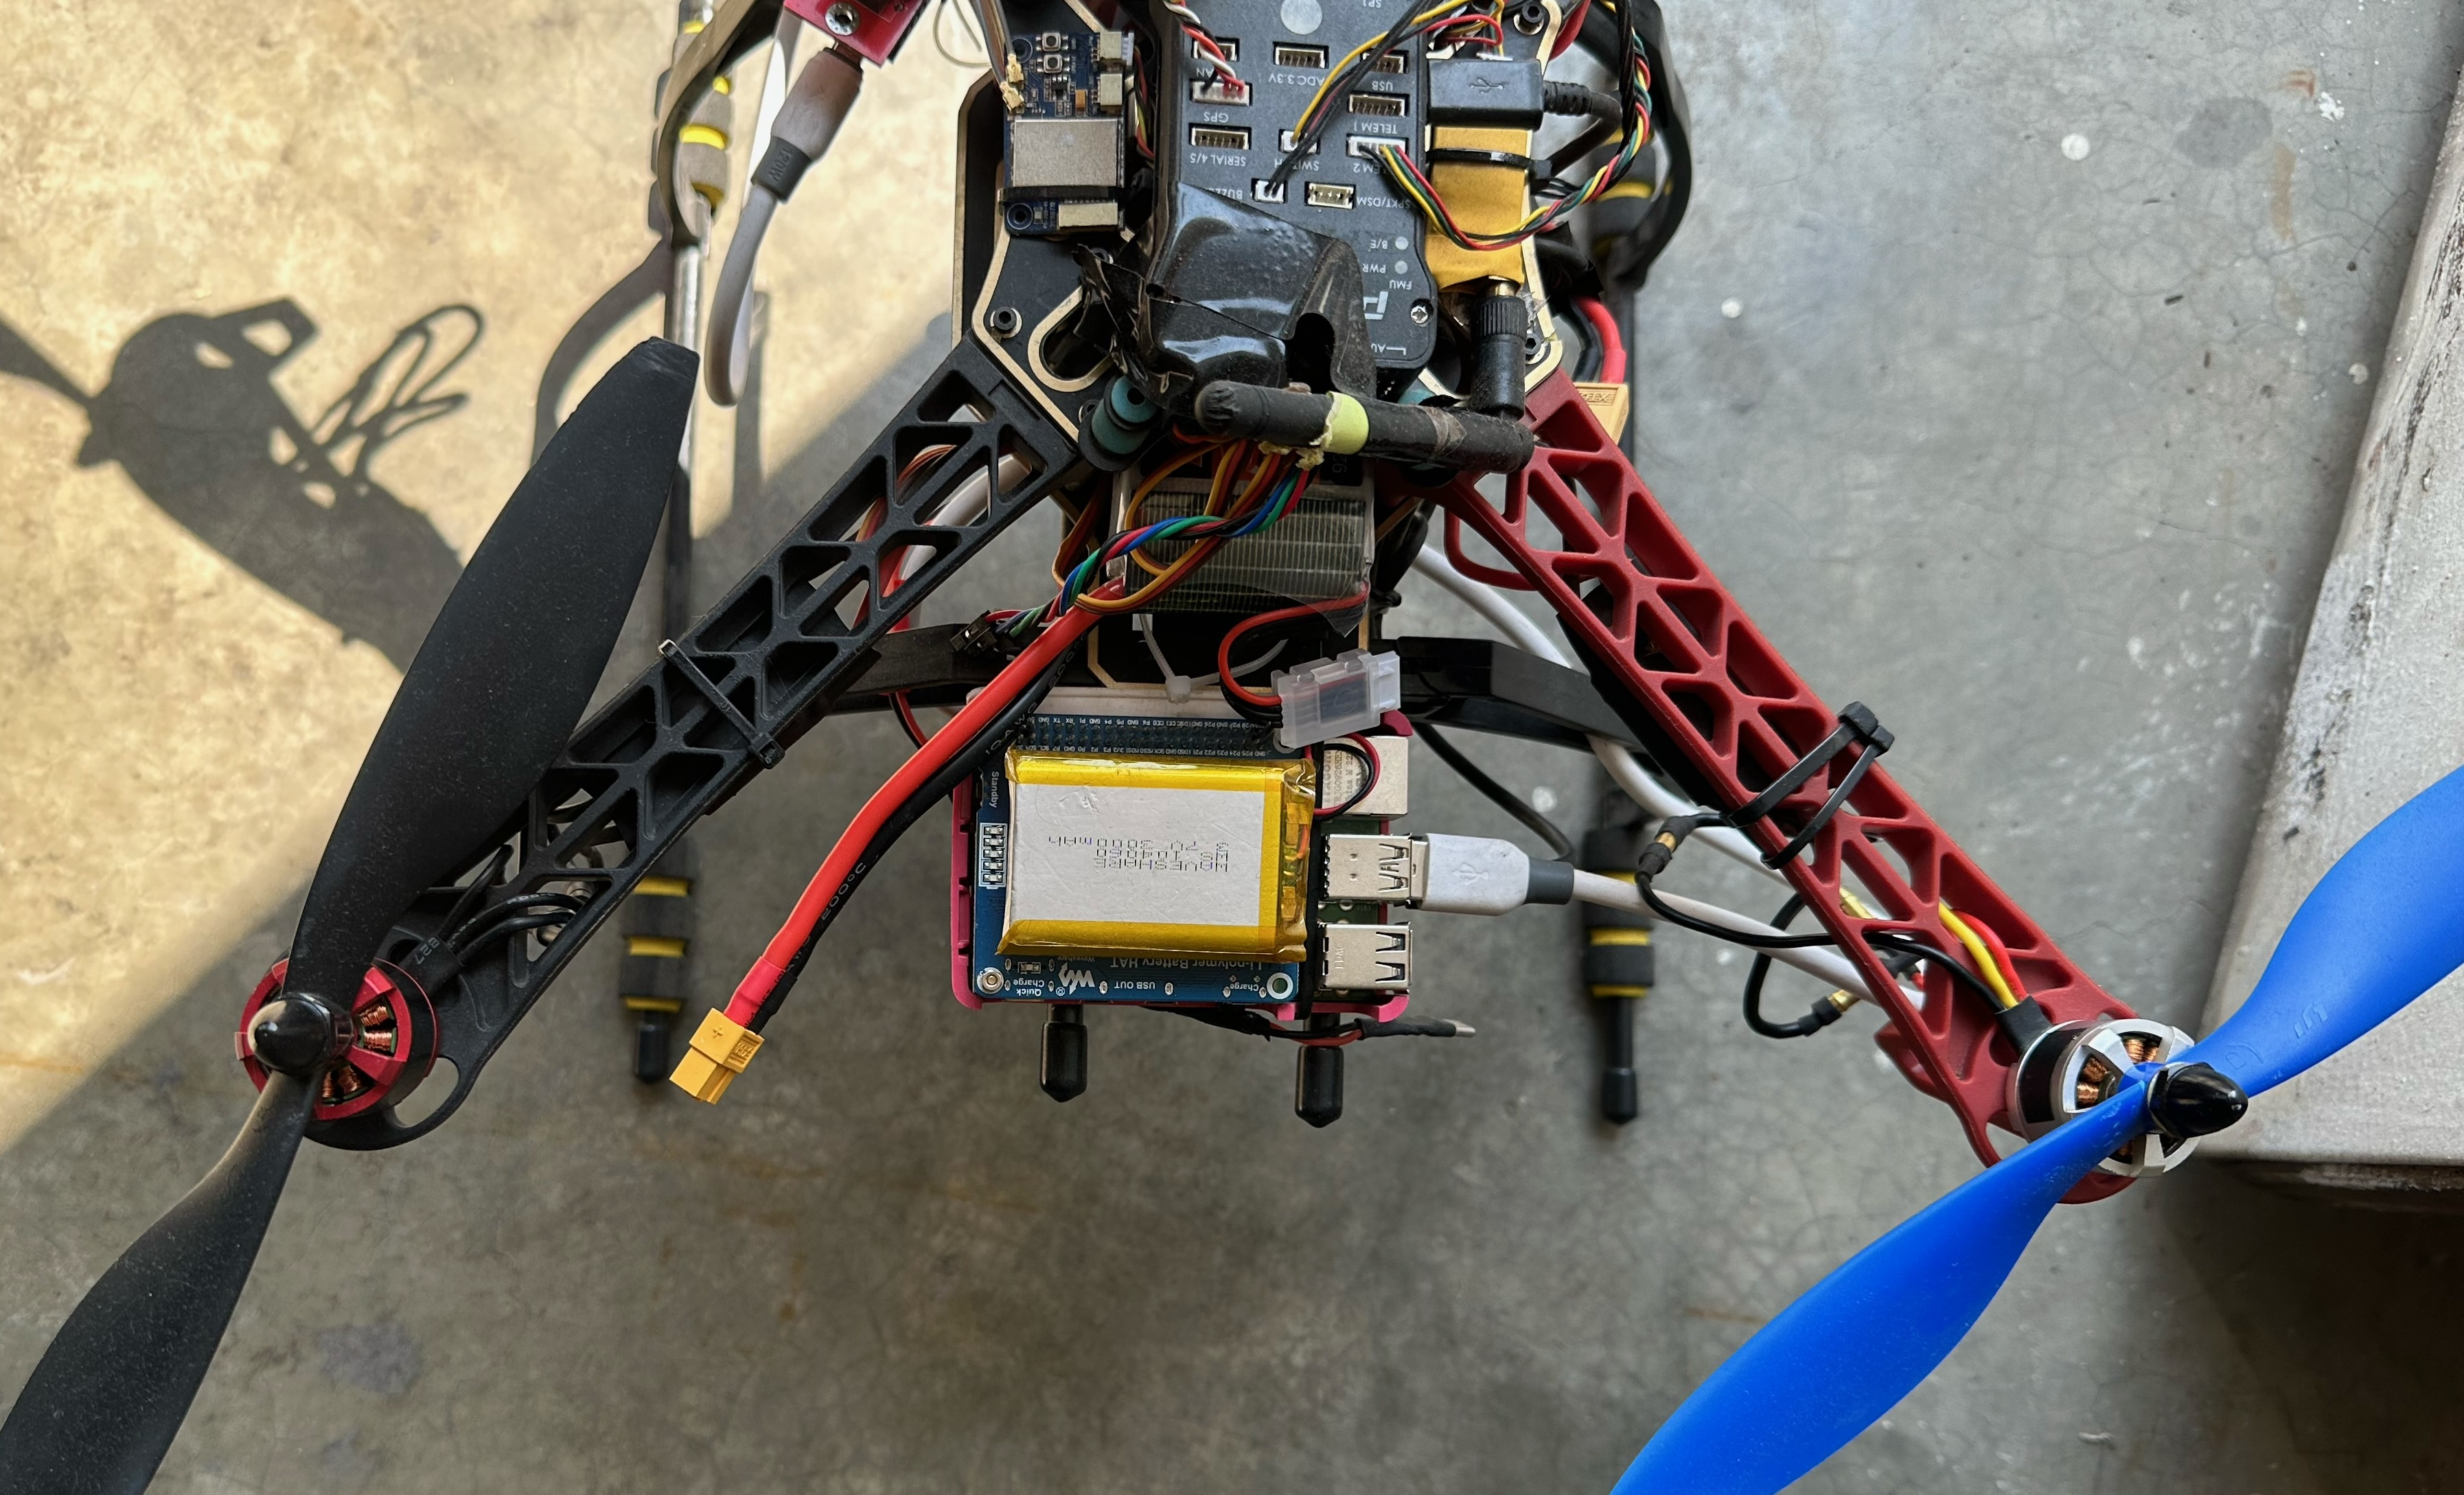
\includegraphics[width=0.45\textwidth]{imagenes/rasp-montada.jpeg}}
        \end{minipage}
    \end{minipage}
    
    \caption{Montaje de la Raspberry Pi4 sobre la placa superior.}
\end{figure}

\noindent Por otra parte, los sistemas de telemetría también son importantes, por lo que para ello se utilizará el módulo NRF24L01. Las características de la telemetría se muestran en la Figura \ref{fig:nrf}:
\noindent Este módulo se puede agregar fácilmente a cualquier sistema MCU/ARM/PIC/AVR/STM32. Además, está diseñado con un amplificador de potencia y antena SMA, lo que le permite utilizar la comunicación inalámbrica hasta a 800 metros (con línea de vista).
\begin{itemize}[itemsep=0pt, parsep=0pt, topsep=0pt, partopsep=0pt]
    \item \textbf{Rango:} 800m de LOS
    \item \textbf{Frecuencia:} 2.4 - 2.5GHz
    \item \textbf{Voltaje de operación:} 3 - 3.6V Max
    \item \textbf{Corriente máxima:} 115mA
\end{itemize}

\noindent Un microcontrolador de anfitrión puede comunicarse y configurar el NRF24L01 a través de una interfaz periférica serial de 4 pines (SPI). Los registros de configuración son accesibles a través de la conexión SPI. Los parámetros configurables incluyen el canal de frecuencia (125 canales seleccionables), la potencia de salida y la velocidad de datos (velocidades de datos: 250kbps, 1Mbps y 2Mbps).

\noindent El regulador de voltaje en el chip acepta voltajes de suministro de 1.9 a 3.6V. El módulo tiene entradas tolerantes a 5V que permiten la conexión directa de los pines SPI.

\noindent El filtrado interno resulta en márgenes altos para cumplir con los estándares regulatorios de RF. La radio del módulo utiliza modulación de desplazamiento de frecuencia gaussiana (GFSK) así como control automático de ganancia rápida (AGC).

\noindent El módulo incluye un pin de solicitud de interrupción (IRQ) que se puede utilizar para despertar al microcontrolador principal del modo de suspensión cuando el módulo recibe una transmisión, lo que proporciona un gran ahorro de energía en dispositivos con batería. 

\begin{figure}[H]
    \centering
    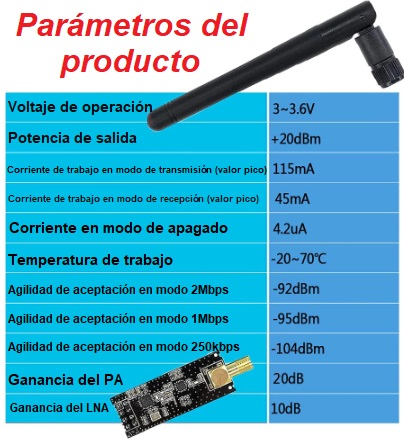
\includegraphics[width=0.6\textwidth, height=7.5cm]{imagenes/parametrosNRF.jpg}
    \caption{Características de la telemetría NRF24L01.}
    \label{fig:nrf}
\end{figure}

\noindent Para cada acción controlable a distancia, se necesita un canal único para transmitir la entrada. El mínimo necesario para pilotar un multirrotor es de cuatro canales: throttle (aceleración), yaw (rotación), pitch (timón) y roll (alerón). Para cada interruptor de modo de vuelo, control de cardán o control de iluminación, se necesita un canal adicional.
\begin{figure}[H]
    \centering
    \includegraphics[width=0.5\textwidth, height=6.5cm]{imagenes/canalización.png}
    \caption{Canalización de Control en Drones Multirrotores.}
    \label{fig:nrf}
\end{figure}

\noindent El Xiangtat Flysky FS-i6X Transmisor con receptor iA6B ayudará a tener un control manual de vuelo para poder controlar el dron desde tierra. El transmisor FS-i6X y el receptor FS-iA6B constituyen un sistema RC computarizado proporcional digital AFHDS 2A de 6 canales. Este sistema ofrece una protección superior contra interferencias mientras mantiene un menor consumo de energía y una alta sensibilidad fiable del receptor. Está especialmente desarrollado para todos los modelos de control de radio. \cite{FLYSKY}

\textbf{Especificaciones del transmisor FS-i6X:}
\begin{itemize}[itemsep=0pt, parsep=0pt, topsep=0pt, partopsep=0pt]
    \item Canales: 6-10 (por defecto 6)
    \item Tipo de modelo: Ala fija/planeador/cuadricóptero
    \item Rango de RF: 2.408 - 2.475 GHz
    \item Potencia RF: < 20dBm
    \item Canal RF: 135
    \item Ancho de banda: 500kHz.
    \item Sistema de 2.4GHz: AFHDS 2A / AFHDS.
    \item Tipo de modulación: GFSK
    \item Resolución del barril: 4096
    \item Advertencia de baja tensión: < 4.2V
    \item Puerto DSC: puerto PS/2
    \item Longitud de la antena: 26mm (antena dual)
    \item Peso: alrededor de 400g
    \item Visualización: visualización transflectiva STN, red LCD de 128 x 64, VA 73 x 39 mm, LCD con retroiluminación blanca
    \item Tamaño: 190 x 174 x 89 mm
    \item Actualización en línea: sí
    \item Certificado: CE0678, FCC ID: N4ZFLYSKYI6X
\end{itemize}
\textbf{Especificaciones del receptor FS-iA6B:}
\begin{itemize}[itemsep=0pt, parsep=0pt, topsep=0pt, partopsep=0pt]
    \item Canales: 6
    \item Rango de RF: 2.4055 - 2.475GHz
    \item Canal RF: 140
    \item Sensibilidad del receptor RF: -105dBm
    \item Ancho de banda: 500kHz
    \item Sistema de 2.4GHz: AFHDS 2A
    \item Tipo de modulación: GFSK
    \item Potencia: 4.0 - 6.5V
    \item Transmisor compatible: FS-i6X, FS-i4, FS-i6, FS-i10, FS-GT2E, FS-GT2G
    \item Longitud de la antena: 26mm (antena dual)
    \item Peso: 16.3g
    \item Tamaño: 47 x 26.2 x 15 mm
    \item Puerto i-bus: sí
    \item Puerto de adquisición de datos: sí
\end{itemize}

\begin{figure}[H]
    \centering
    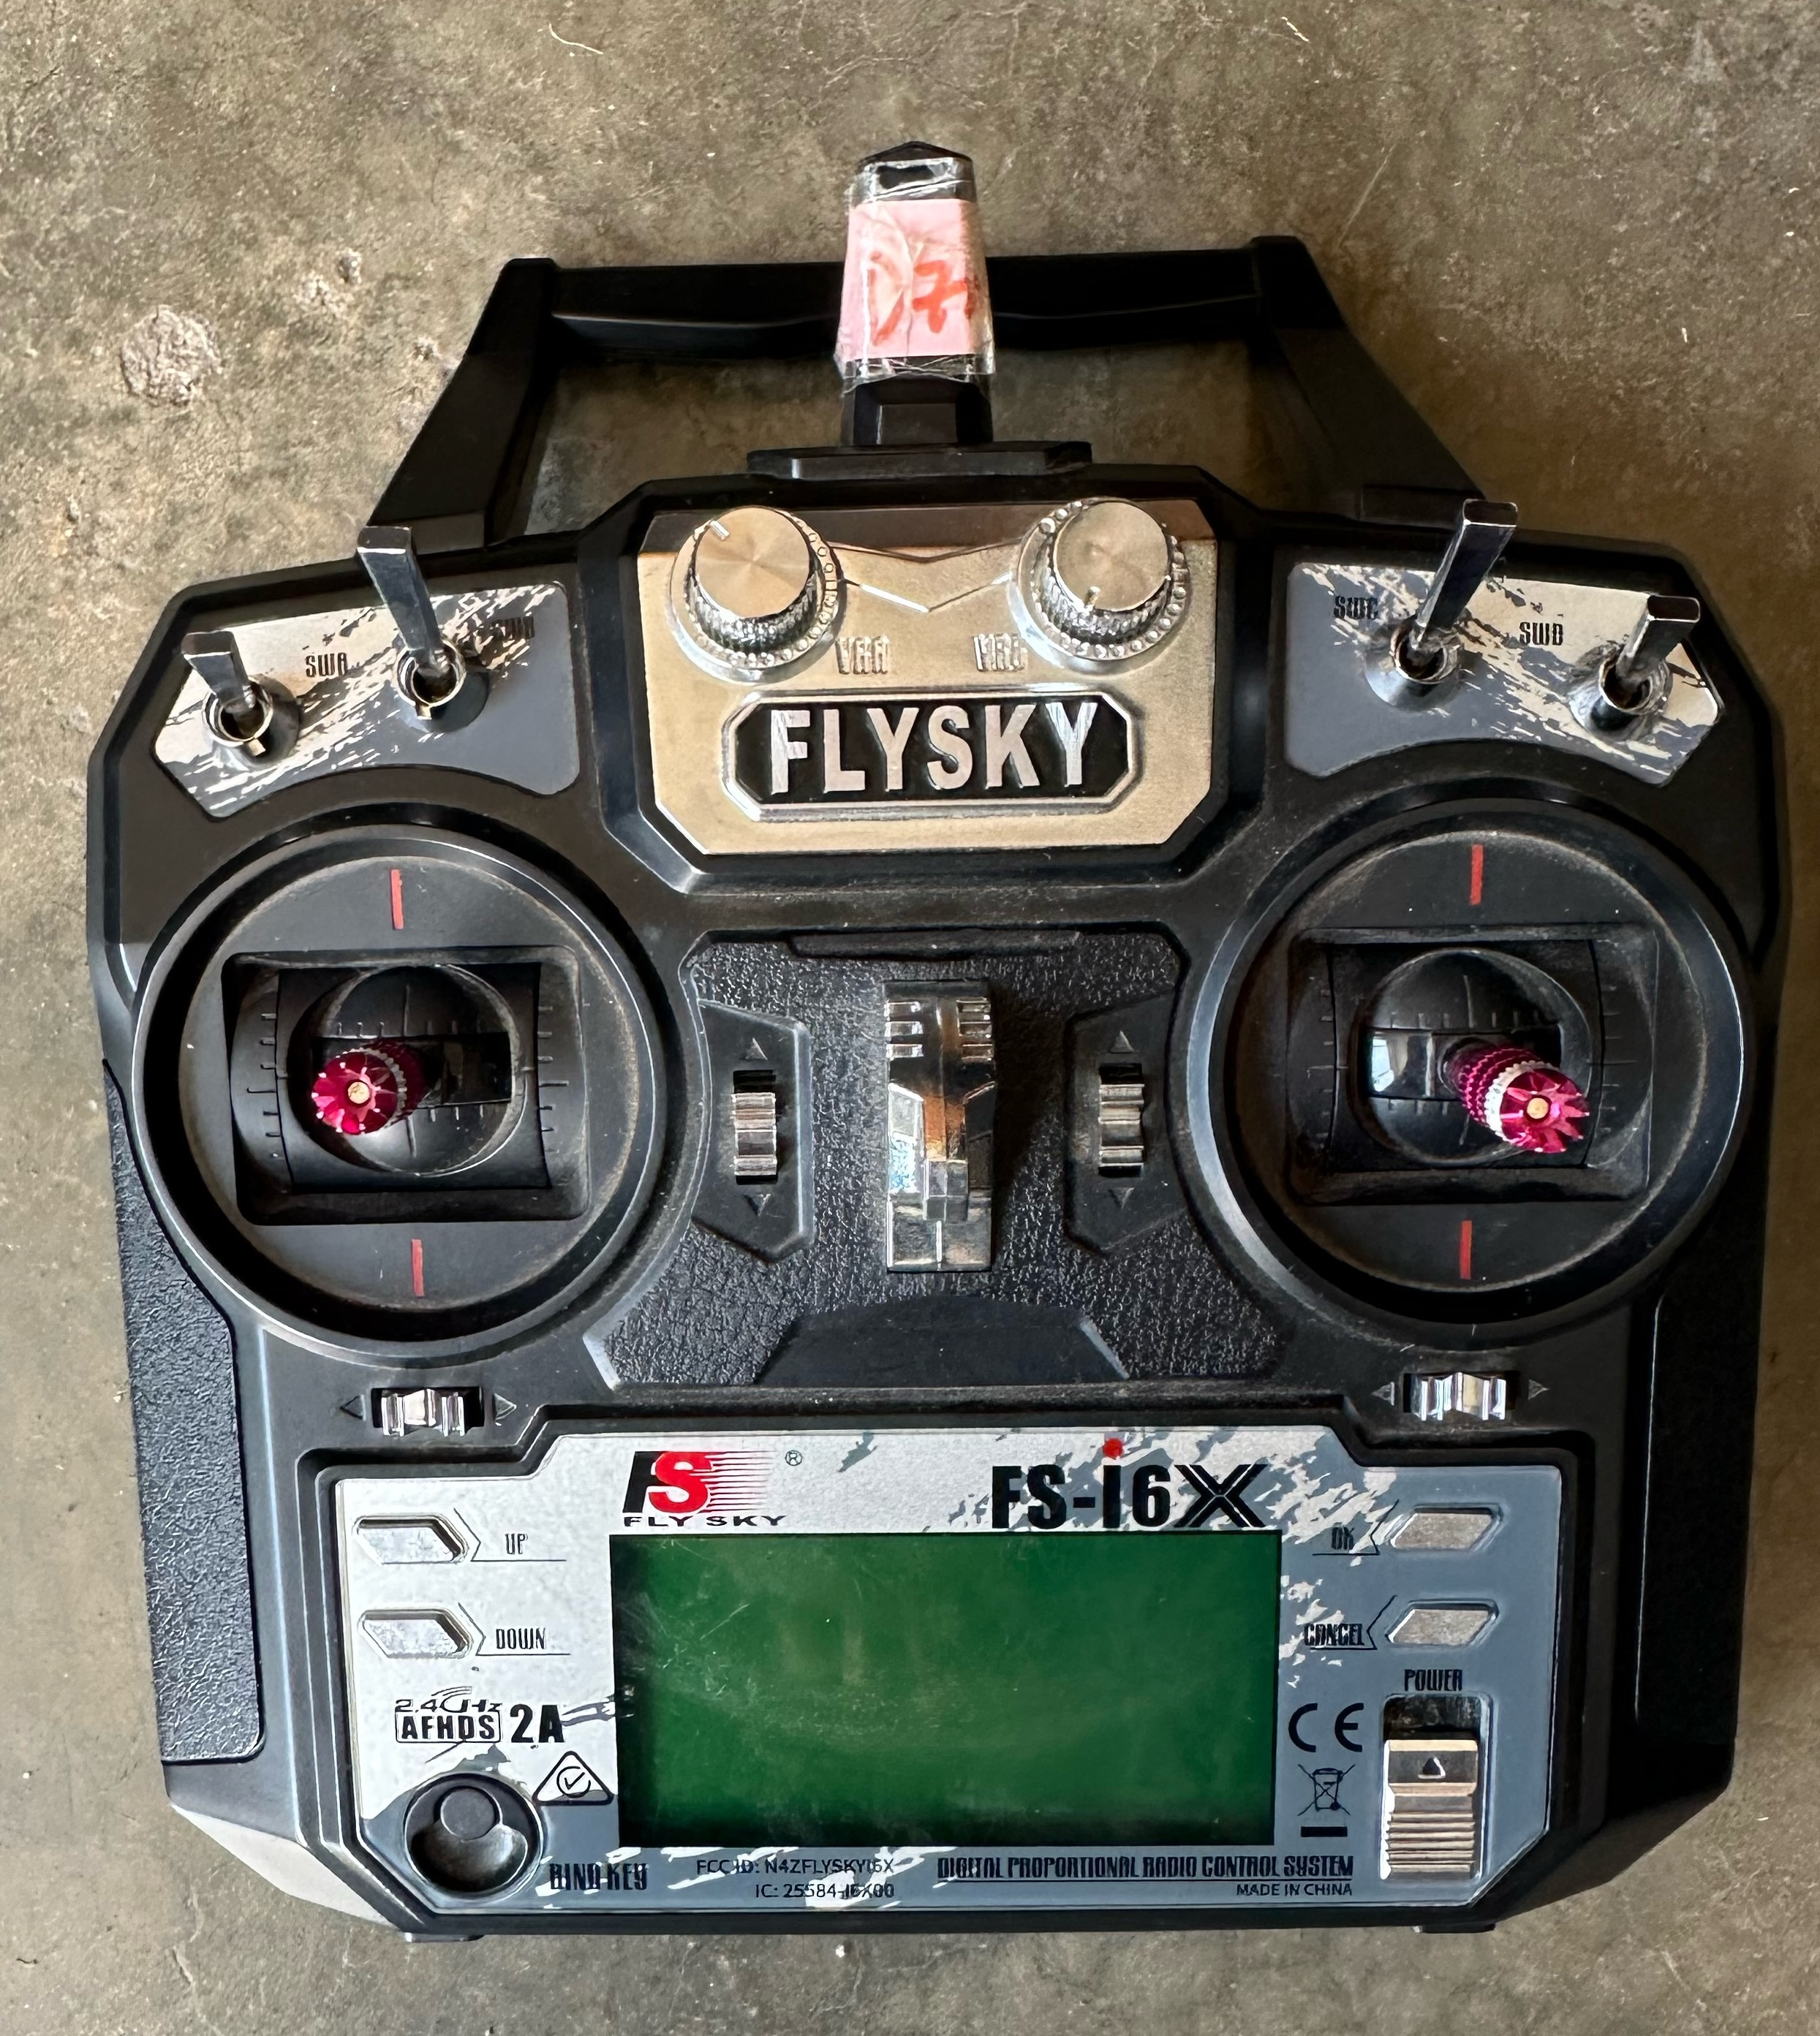
\includegraphics[width=0.45\textwidth]{imagenes/control.jpeg}
    \caption{Transmisor Radio Controlado.}
    \label{fig:control}
\end{figure}

\noindent En cuanto a la batería del dron, esta se coloca ajustadamente entre la placa inferior y la placa superior para evitar su deslizamiento. Tomando en cuenta que para no reducir su tiempo de vida, no se debe permitir que sus celdas se descarguen menos del 80\% (para una batería de 12V no se debe descargar a menos de 9.6V). Su capacidad y corriente por hora dependen del consumo energético del UAV:
\begin{itemize}
    \item Entre más grande más consumo
    \item Entre más propelas más consumo
    \item Entre más dispositivos conectados, más consumo
    \item Entre más velocidad y movimiento, más consumo
\end{itemize}

\begin{table}[H]
    \centering
    \caption{Relación de la capacidad de la batería con el tamaño de las hélices.}
    \begin{tabular}{|c|c|}
        \hline
        \cellcolor[HTML]{C0C0C0}Tamaño de las hélices & \cellcolor[HTML]{C0C0C0}Capacidad de la batería \\
        \hline
        6” & 1500 mAh a 2200 mAh \\
        \hline
        5” & 1300 mAh a 1800 mAh \\
        \hline
        4” & 850 mAh a 1300 mAh \\
        \hline
        3” & 650 mAh a 1000 mAh \\
        \hline
    \end{tabular}
    \label{tab:battery_helices}
\end{table}

\noindent El tiempo de vuelo está relacionado al consumo energético de la batería y se puede calcular a partir de la corriente que consume el dron, la batería, el peso, la mínima descarga del dron, etc. Existen modelos matemáticos (e.g. Backstepping) y simuladores (e.g. ROS Gazebo) que pueden predecir el consumo energético de un UAV \cite{videodron}.

\begin{figure}[H]
    \centering
    \subfigure[) Individualmente.]{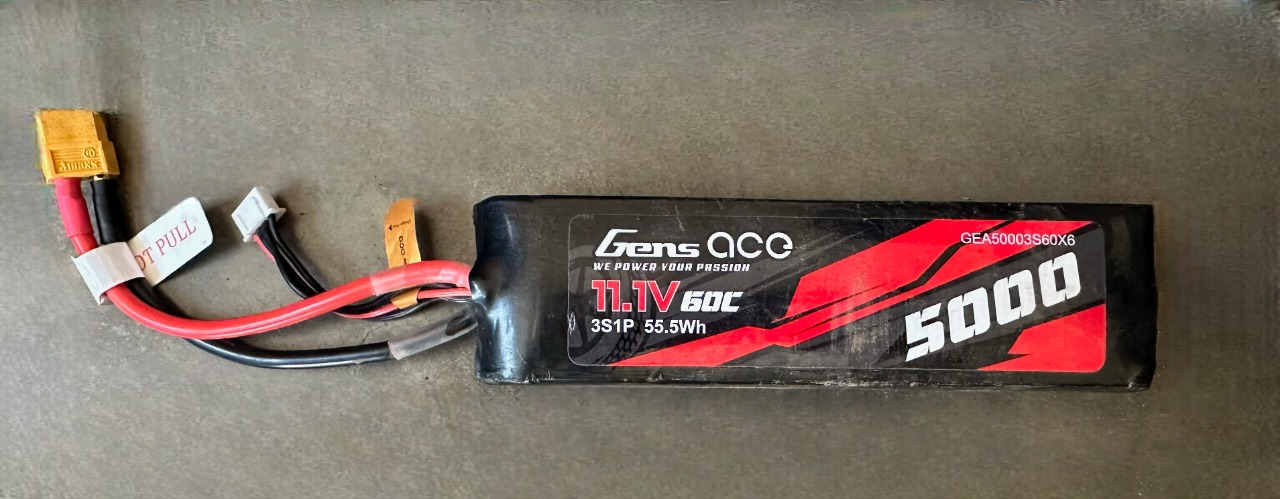
\includegraphics[width=0.45\textwidth, height=4cm]{imagenes/bateria.jpeg}}
    \quad
    \subfigure[) Montada.]{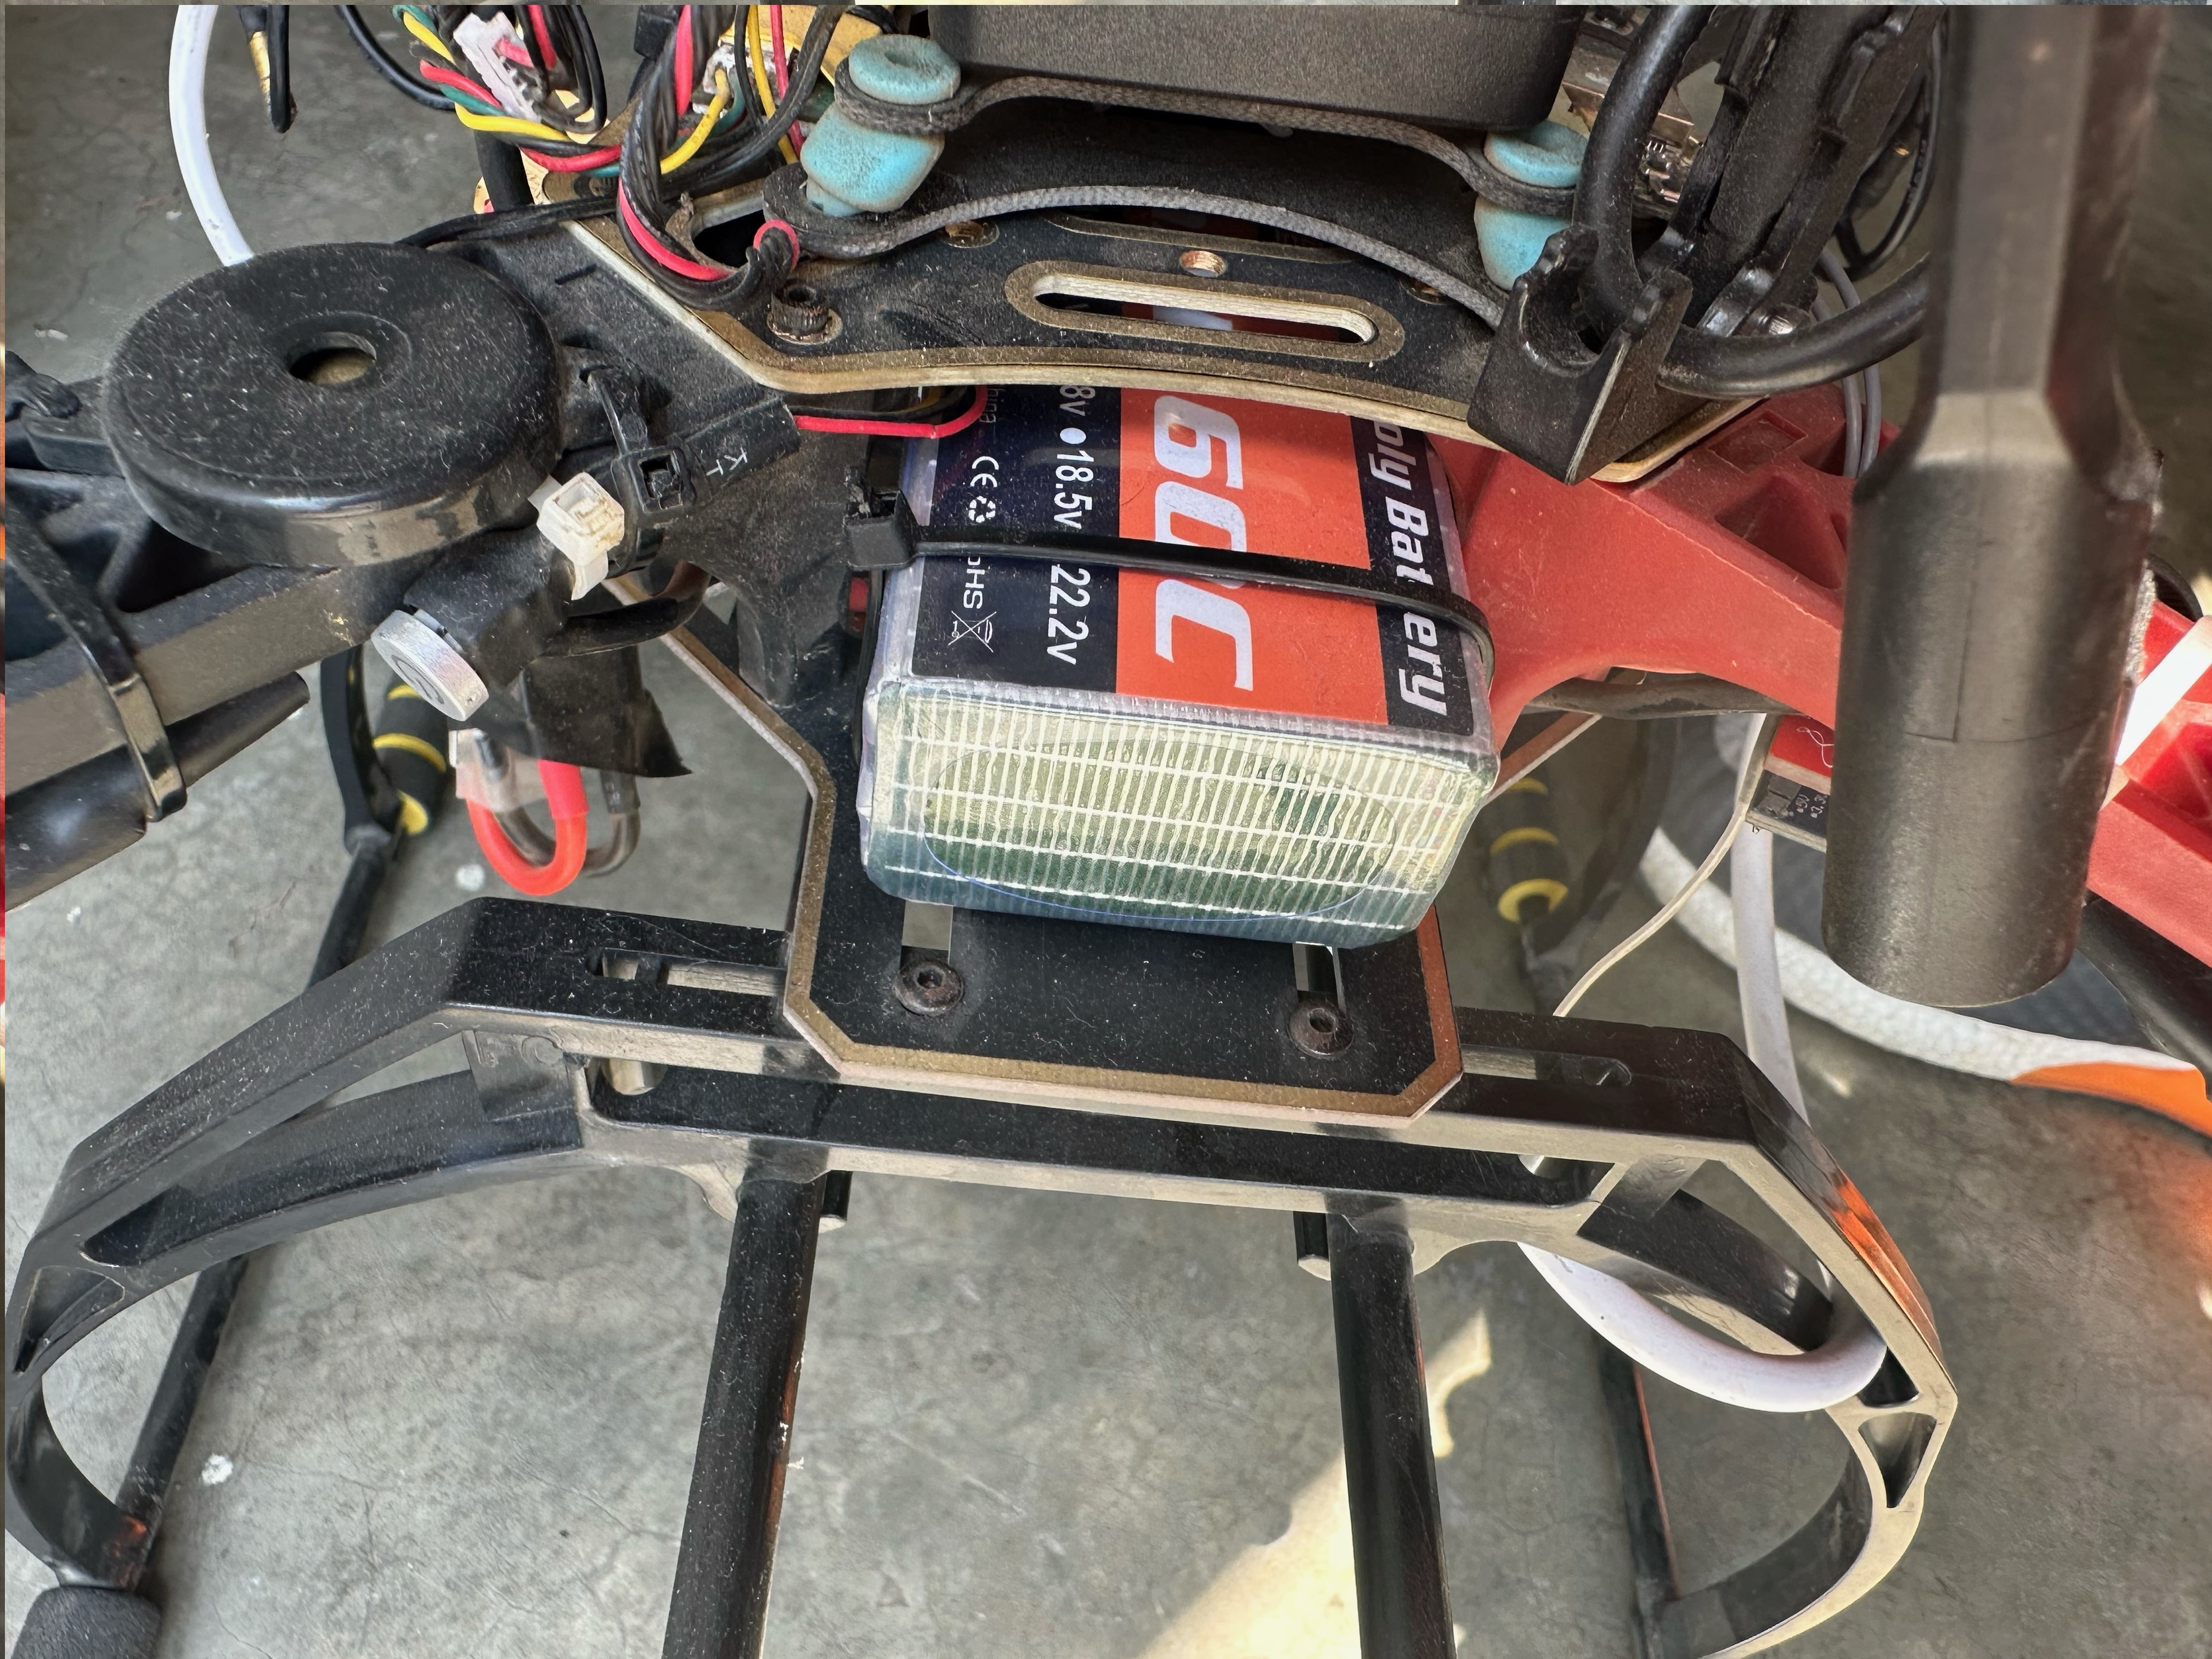
\includegraphics[width=0.45\textwidth, height=4cm]{imagenes/bateria-montada.jpeg}}
    \caption{Montaje de la batería 5000mAh 6 celdas 22.2v 25C-60C RC sobre la placa inferior.}
    \label{fig:bateria}
\end{figure}


\noindent Ya por último, podemos ver en la Figura \ref{fig:drone} el dron completamente armado con todos los componentes ensamblados y montados sobre la estructura y las placas del dron.

\begin{figure}[H]
    \centering
%    \includegraphics[width=0.5\textwidth]{imagenes/}
    \caption{Dron listo para pruebas de vuelo.}
    \label{fig:drone}
\end{figure}

\noindent Estos mismos procesos se hacen para el ensamblado de los otros dos prototipos, más adelante se seguirán haciendo pruebas y documentación sobre las demás actividades para modelar el consumo energético y los esquemas de vuelo para la recolección de datos.
\begin{figure}[H]
    \centering
    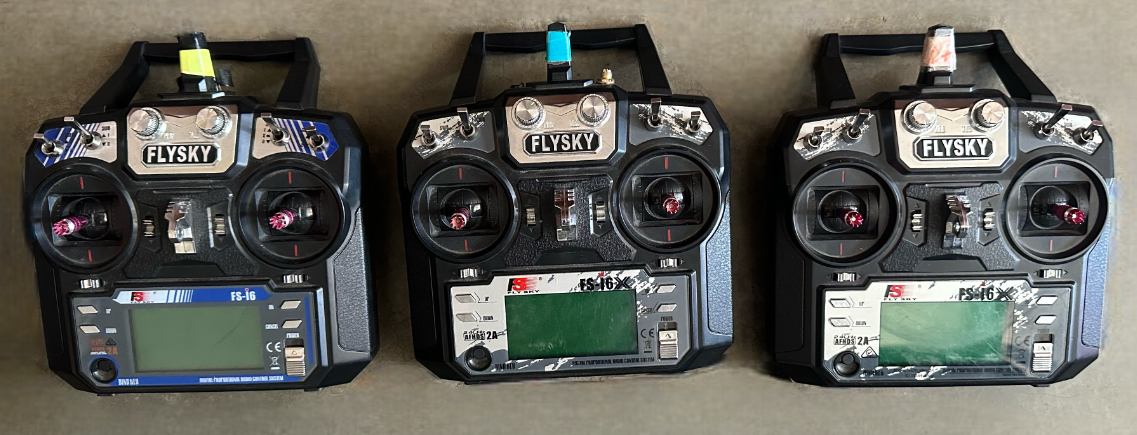
\includegraphics[width=0.85\textwidth]{imagenes/controles.png}
    \caption{Transmisores de Radio Control para cada dron .}
    \label{fig:drones}
\end{figure}
\begin{figure}[H]
    \centering
    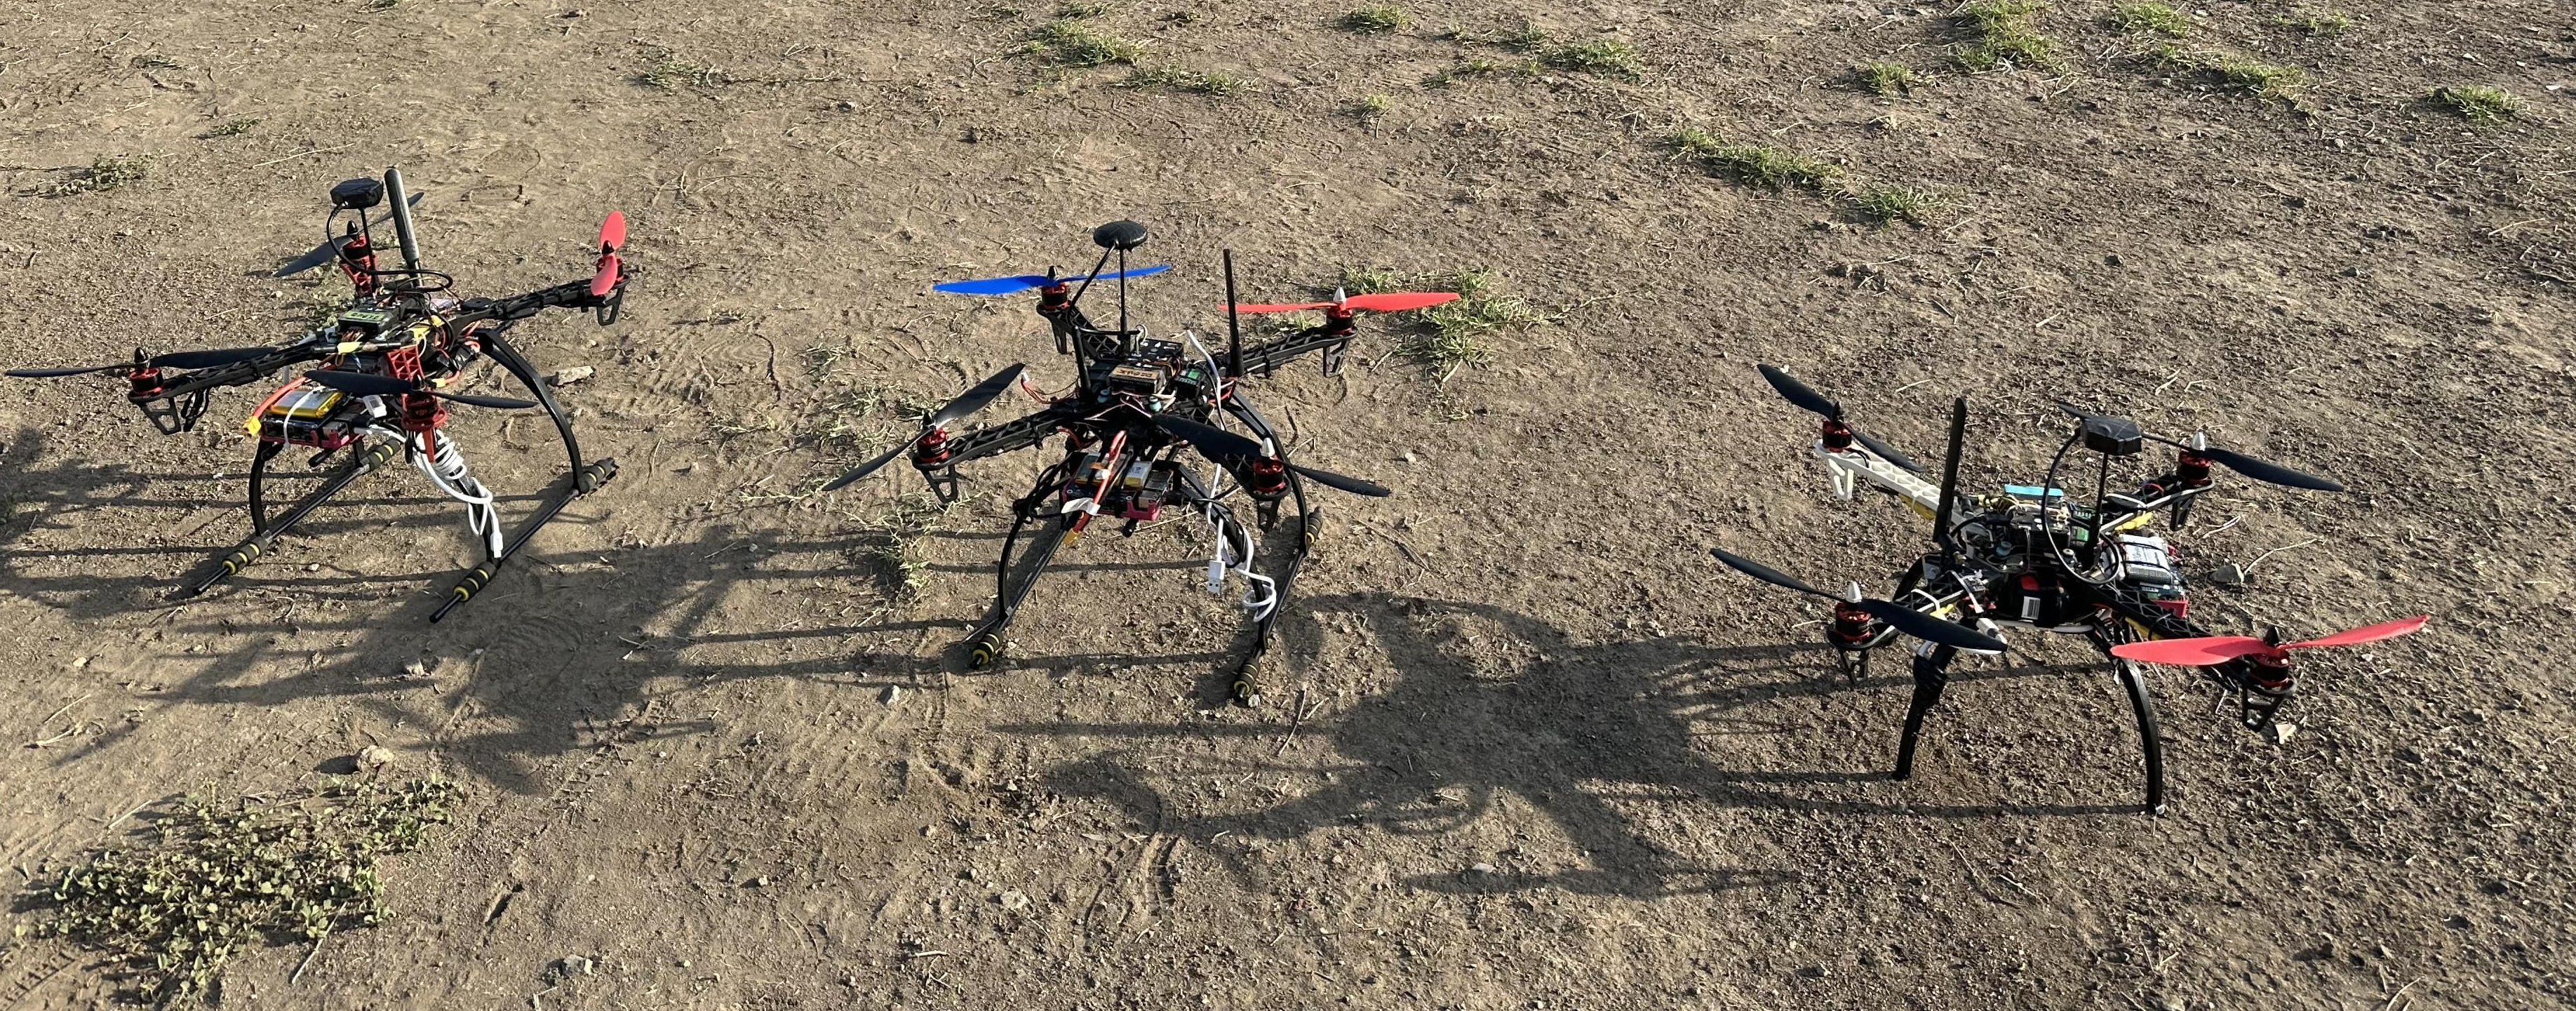
\includegraphics[width=0.85\textwidth, height=6cm]{imagenes/tres-drones.jpg}
    \caption{Drones listos para pruebas de vuelo.}
    \label{fig:drones}
\end{figure}

\noindent Por último, se describe el proceso de vuelo coordinado del enjambre de drones en el diagrama de flujo de la Figura \ref{fig:diagrama-vuelo-enjambre}. Comenzando con la inicialización de los dispositivos involucrados, donde, se encienden los tres drones, que consisten en el dron líder y los dos drones seguidores. Simultáneamente, la estación base se conecta a un monitor serial, lo que permite la comunicación con el dron líder desde la estación base.

\noindent Una vez encendidos los drones, cada uno de ellos obtiene sus coordenadas GPS. Los drones seguidores envían sus coordenadas al dron líder, quien recopila y envía estas coordenadas junto con las propias a la estación base. Este ciclo de envío de coordenadas se repite continuamente hasta estas que todas se reciban en la estación base y se muestren en el monitor serial.

\noindent La estación base verifica entonces si ha recibido todas las coordenadas necesarias. No se puede continuar el proceso si no se han recibido las coordenadas de todos los drones en la estación base. 

\noindent Una vez que la estación base ha recibido todas las coordenadas, se envía un comando de inicio al dron líder. Este comando indica al dron líder que debe prepararse para iniciar el vuelo coordinado. Si el comando ha sido recibido correctamente, el dron líder envía un comando de despegue a los drones seguidores para que todos los drones despeguen simultáneamente.

\noindent Una vez en vuelo, cada dron sigue su ruta programada. Este seguimiento de ruta se mantiene mientras el vuelo esté en progreso, asegurando que los drones se desplacen de acuerdo con sus planes de vuelo configurados. Finalmente, el proceso concluye cuando los drones regresan a la estación base, finalizando el procedimiento de vuelo en enjambre o coordinado.

\begin{figure}[H]
    \centering
    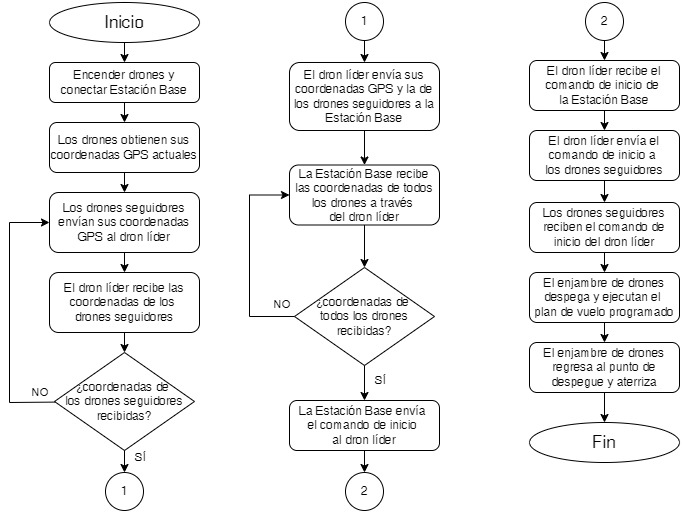
\includegraphics[width=0.95\textwidth]{imagenes/diagrama-enjambre.jpg}
    \caption{Diagrama de flujo para el vuelo en enjambre.}
    \label{fig:diagrama-vuelo-enjambre}
\end{figure}


\section{Implementación de la WSN}
\subsection{Adquisición de los Elementos}
En esta etapa, se procederá con la adquisición de los elementos esenciales para la implementación de la WSN, basándonos en las selecciones detalladas durante el análisis y diseño del proyecto:
\begin{enumerate}
    \item \textbf{Termistor LM35 (temperatura):} Utilizado para monitorear la temperatura ambiental y su análisis podría indicar algún impacto en el comportamiento de las especies.
    \item \textbf{Módulo GPS Neo-6M (geolocalización):} Necesario para rastrear y registrar la ubicación geográfica precisa de las especies, proporcionando información vital sobre la distribución espacial y migración de las especies.
    \item \textbf{Cámara Trampa PR-700 (video): } Esencial para obtener imágenes de alta resolución que facilitarán la identificación de especies y el análisis de su actividad y comportamientos.
    \item \textbf{Arduino Pro Micro (microcontrolador):} Elegido por su bajo consumo energético, capacidad suficiente para tareas específicas del proyecto y tamaño compacto.
    \item \textbf{Módulos LoRa UART 868/915 MHz (transmisión de datos):} Seleccionados por su capacidad única para proporcionar conectividad confiable a larga distancia con bajo consumo de energía.
    \item \textbf{Baterías LiPo recargables (fuente de energía):} Seleccionadas por su buen funcionamiento y larga duración, ofreciendo una solución confiable para dispositivos de monitoreo autónomos.
    \item \textbf{Módulo MicroSD Card Adapter MLMSD (adaptador):} Elegido por su compatibilidad con tarjetas MicroSD, proporcionando capacidades de almacenamiento significativas y fácil integración con microcontroladores.
    \item \textbf{Memorias MicroSD (almacenaje de datos):} Utilizadas para el almacenamiento de datos generados por los sensores y archivos de video de las cámaras trampa.
\end{enumerate}
A continuación, se presenta la tabla comparativa \ref{tabla:precioswsn} que resume los precios y proveedores de cada elemento necesario, con su respectivo hipervínculo:

\begin{table}[H]
  \centering
  \caption{Comparación de precios de componentes electrónicos}
  \begin{tabular}{|l|l|l|l|}
    \hline
    \cellcolor[HTML]{C0C0C0}\textbf{Elemento} & \cellcolor[HTML]{C0C0C0}\textbf{Amazon} & \cellcolor[HTML]{C0C0C0}\textbf{Mercado Libre} & \cellcolor[HTML]{C0C0C0}\textbf{AliExpress} 
    \\ \hline
    Arduino Pro Micro & \$243.00 [\href{https://www.amazon.com.mx/Arduino-Nano-Every-Single-Board/dp/B07VX7MX27/ref=sr_1_3?__mk_es_MX=%C3%85M%C3%85%C5%BD%C3%95%C3%91&crid=307WLXDB631RV&dib=eyJ2IjoiMSJ9.wzfOzm2PL4-zMZ2NN_5BNdR4mDrlSoSOwDLjWcQn9VI4HLku1uxkwYmK6IsZr0xutdI9rmfjBP6GgqhL1reGWB8UoHG6Od8i3xY89uacfvcPGP6-V-2P9SODLnx_0QMijWGI0iT89I0QFjZN9QNvkmCBkQp29V-JNl8GAy2cjAGWzRCRvh0jf78M0DHjbvdrbVZGE2n4M46X2HsC9Nby-mmLOzduvvx3IfTJWFX3ZEhJKyJZxuH06SEP12uh4KzFa9VwFyrzpoqp8bpKrSc5nTBClJrSTum85Uz8CvnsVZE.gSmbVutZeovDlO7E4ayAcklEYu1di6ULkI-0w1CPP38&dib_tag=se&keywords=Arduino%2BPro%2BMicro&qid=1710144626&sprefix=arduino%2Bpro%2Bmicro%2Caps%2C252&sr=8-3&ufe=app_do%3Aamzn1.fos.4e545b5e-1d45-498b-8193-a253464ffa47&th=1}{Amazon}] & \$175.50 [\href{https://articulo.mercadolibre.com.mx/MLM-1941648223-tarjeta-leonardo-pro-micro-16mhz-5v-compatible-con-arduino-_JM#position=6&search_layout=stack&type=item&tracking_id=00e5ebad-5e49-4afc-bd81-e6c056af7411}{Mercado Libre}] & \$65.09 [\href{https://es.aliexpress.com/item/1005005234161130.html?spm=a2g0o.productlist.main.3.4980Q434Q434c4&algo_pvid=7d1f91e3-002d-456e-9407-d23756667968&aem_p4p_detail=2024031101101816580952553541430004787116&algo_exp_id=7d1f91e3-002d-456e-9407-d23756667968-1&pdp_npi=4%40dis%21MXN%2165.09%2165.09%21%21%213.80%213.80%21%402101fb1417101446189377471e211f%2112000032305530340%21sea%21MX%210%21AB&curPageLogUid=d7dvSAouEC8o&utparam-url=scene%3Asearch%7Cquery_from%3A&search_p4p_id=2024031101101816580952553541430004787116_2}{AliExpress}] \\ \hline
    Termistor LM35 & \$40.00 [\href{https://www.amazon.com.mx/Precision-Centigrade-Temperature-Sensors-original/dp/B07VZ567YJ/ref=sr_1_8?__mk_es_MX=%C3%85M%C3%85%C5%BD%C3%95%C3%91&crid=130LLR8OJMASG&dib=eyJ2IjoiMSJ9.jFfBJnZAJqV6Q6JweL1uxoGmt6vmVyVuMFf6ko5tbTh9M3i2NMnBBzqp83CvScdrxLixD41-Tu1nc_9rcKxUvnXySlsrbJtx-4kXTDFVwhCZLLo-om2UFoZiRr6znJm5PUfpUR6-TunS0olQH4R2WYhnhfVNcZdFG6YAYmDepTf5S_y8VVKvmCgI4Ch5QBeH1wpHS6oKOJ7w6gn5o4xkH_37O1hsPXs18Hjbx0WMuFggfkwDUGREEOOH3Kfir_xlPK4GzZkCftaVdslRgQh-jj00S8cy4TwL18Ps1-US8M0.J1_A7vUWx5dlHfUiQUYMtFrIr4oNVspGhi0ZarDJznk&dib_tag=se&keywords=Termistor+LM35&qid=1710143659&sprefix=termistor+lm35%2Caps%2C207&sr=8-8}{Amazon}] & \$63.50 [\href{https://articulo.mercadolibre.com.mx/MLM-839463622-sensor-de-temperatura-lm35-dz-_JM#position=32&search_layout=grid&type=item&tracking_id=d6f18b96-6c7c-47c4-8ed0-cef8096f5927}{Mercado Libre}] & \$25.86 [\href{https://es.aliexpress.com/item/1005004825930346.html?spm=a2g0o.productlist.main.39.50cdprYxprYxX7&algo_pvid=91a52733-c6a4-4fc3-b3c8-fe28fdf689eb&aem_p4p_detail=202403110057211467828156373050004809487&algo_exp_id=91a52733-c6a4-4fc3-b3c8-fe28fdf689eb-19&pdp_npi=4%40dis%21MXN%2131.51%2125.86%21%21%211.84%211.51%21%402101fb1417101446189377471e211f%2112000032305530340%21sea%21MX%210%21AB&curPageLogUid=d7dvUmDO4G8x&utparam-url=scene%3Asearch%7Cquery_from%3A&search_p4p_id=202403110057211467828156373050004809487_2}{AliExpress}] \\ \hline
    Módulo GPS Neo-6M & \$119.00 [\href{https://www.amazon.com.mx/Neuftech-NEO-6M-GPS-Receiver-STM32-Arduino/dp/B01MYVG3P5/ref=sr_1_3?__mk_es_MX=%C3%85M%C3%85%C5%BD%C3%95%C3%91&crid=1TFZ78IGIQNVF&dib=eyJ2IjoiMSJ9.-i5lTPNtYdUCJy1dxg7GJxYQFmQ3KgpnoyKhLQmb57X5PndCaxvg2Id-Tmo8V4xlxNGaRksD_ySuQ9CHP_2zHtCbXnlmbFLC04dvwHhdN_4EkkPQGNEwqXlHoQg2-jKLz_MLRCb9SD5hWiAlzSuvxuGHZyjw7bfu1KLVVtLIhigfRXbpPANmEGSV9JZr8wB9nEnl9k4Rhw9hCrThrl4X4uXyNhT_4fyj0qMTiFRCY7-_RWSzRf-yYr82Iw9GLapxrPh4J3zXWQUVT6W_4L_gDudLF7dWkPlu4e5x7RYTTrQz5TjH8RicX9_XeVwwE.DsWg90xkz47l8wzHOG5iYVwnTDE1E-EmXCIRX3R06ZM&dib_tag=se&keywords=NEO-6M&qid=1710143727&sprefix=neo-6m%2Caps%2C201&sr=8-3}{Amazon}] & \$149 [\href{https://articulo.mercadolibre.com.mx/MLM-677336119-modulo-gps-neo-6m-gy-gps6mv2-para-arduino-pic-raspberry-pi-_JM#position=4&search_layout=stack&type=item&tracking_id=00e5ebad-5e49-4afc-bd81-e6c056af7411}{Mercado Libre}] & \$72.62 [\href{https://es.aliexpress.com/item/1005004438292781.html?spm=a2g0o.productlist.main.1.2cfb4b1cU5qbmZ&algo_pvid=91a52733-c6a4-4fc3-b3c8-fe28fdf689eb&aem_p4p_detail=202403110057211467828156373050004809487&algo_exp_id=91a52733-c6a4-4fc3-b3c8-fe28fdf689eb-1&pdp_npi=4%40dis%21MXN%2172.62%2172.62%21%21%215.85%215.85%21%402101fb1417101446189377471e211f%2112000032305530340%21sea%21MX%210%21AB&curPageLogUid=d7dvUmDO4G8x&utparam-url=scene%3Asearch%7Cquery_from%3A&search_p4p_id=202403110057211467828156373050004809487_2}{AliExpress}] \\ \hline
    Cámara Trampa PR-700 & \$1,309.64 [\href{https://www.amazon.com.mx/1080P-Trail-Camara-Caza-Vision/dp/B07R7Z5X12/ref=sr_1_1?__mk_es_MX=%C3%85M%C3%85%C5%BD%C3%95%C3%91&crid=1R0S82IBX5JLD&dib=eyJ2IjoiMSJ9.MDHzttm1r5hzXwqff8s0xXxtbVtC7Y5dSLr4ejodQOFXRYgRUdZsTBe1f14ZB-0nxYIhnb3qPzsjGg1XzQjeUXm1NwP9z-TlkiWFOqHtw9f9ImSyRA05do-IwevGMD6nUTR-Bfl-vS55JNrswUiyHb_1TyPK5vo6W-79L-zA4vqIAbJ6ZcGWbbYri__vsf-Jb0Ku6yigXT1G4AqkZ5X2-nwGb0Bd4ujXQKd_2tECmk7bPJ5JKSYLpRlBndVV7xJP7qIr1tpXUyoGocGfF-LgXXHwTq4xFw.4Hk_y6TZTQjyVm2vzfrN9wJkv8aFZoZszn7EwULtqVg&dib_tag=se&keywords=c%C3%A1mara+trampa&qid=1710144371&sprefix=c%C3%A1mara+tra%2Caps%2C243&sr=8-1}{Amazon}] & \$770.65 [\href{https://articulo.mercadolibre.com.mx/MLM-657680742-camara-trampa-hc801g-16mp-celular-infrarrojo-piezo-gsm-1080p-_JM#position=1&search_layout=grid&type=item&tracking_id=00e5ebad-5e49-4afc-bd81-e6c056af7411}{Mercado Libre}] & \$234.37 [\href{https://es.aliexpress.com/item/1005003196329359.html?spm=a2g0o.productlist.main.5.26d34717R8y5R9&algo_pvid=eb8c5605-2939-4b13-bc4b-9a3e07e7a2ec&aem_p4p_detail=202403110057211467828156373050004809487&algo_exp_id=eb8c5605-2939-4b13-bc4b-9a3e07e7a2ec-1&pdp_npi=4%40dis%21MXN%21234.37%21234.37%21%21%2111.78%2111.78%21%402101fb1417101446189377471e211f%2112000032305530340%21sea%21MX%210%21AB&curPageLogUid=d7dvUmDO4G8x&utparam-url=scene%3Asearch%7Cquery_from%3A&search_p4p_id=202403110057211467828156373050004809487_2}{AliExpress}] \\ \hline
    Módulos LoRa & \$353.50 [\href{https://www.amazon.com.mx/DRF1278DM-WX-DRF1278DM-WX915-Long-Range-Transceiver/dp/B07VTVV8G8/ref=sr_1_6?__mk_es_MX=%C3%85M%C3%85%C5%BD%C3%95%C3%91&crid=11JCGW93RMYOS&dib=eyJ2IjoiMSJ9.jxvL2e6CxkW43ZbNjNLjGTD0M9Nx9sRerR6vmj1f18CvF3I-dYRzsUV0PIcArbFtsDVQqHswC7kKZWKhL5EkulL-tO-1fb7g-15mT83wlJaR3Ek3uzUX_vuUw-T1a1wHThp00X3ZxHIdin-l_7cHWhM0yrzBB-0vYwKbgqXCE1s6-02EPR3rIf6x6hFkG8vS0otzdB-k55x53uOKMv0jKpjGb-Wog7C-r4j4rVLaIiS2ot5j5qoFDb1aI6qBKQ5pbNLpCJbqSBL-J0PLtXU-cISbGnGIEfA_HD4YJEI.UhbZ9O-8jJKf0C6VCpx8xeqkIMATBGVTszA5u5gkFbg&dib_tag=se&keywords=m%C3%B3dulo+lora&qid=1710144415&sprefix=m%C3%B3dulo+lora%2Caps%2C246&sr=8-6}{Amazon}] & -------------------- & \$59.09 [\href{https://es.aliexpress.com/item/1005005041209461.html?spm=a2g0o.productlist.main.2.4bba8a17dAjEJY&algo_pvid=09177cb8-446f-400e-8dd7-f5a29445c92a&aem_p4p_detail=2024031101101816580952553541430004787116&algo_exp_id=09177cb8-446f-400e-8dd7-f5a29445c92a-0&pdp_npi=4%40dis%21MXN%2159.09%2159.09%21%21%212.66%212.66%21%402101fb1417101446189377471e211f%2112000032305530340%21sea%21MX%210%21AB&curPageLogUid=d7dvSAouEC8o&utparam-url=scene%3Asearch%7Cquery_from%3A&search_p4p_id=2024031101101816580952553541430004787116_2}{AliExpress}] \\ \hline
    Módulo adaptador MicroSD & \$22.99 [\href{https://www.amazon.com.mx/LEORX-Adaptador-conector-micro-SD-convertidor/dp/B01189N29A/ref=sr_1_4?__mk_es_MX=%C3%85M%C3%85%C5%BD%C3%95%C3%91&crid=2IE9B9Q0K0FHZ&dib=eyJ2IjoiMSJ9.f0jv3XQ9CzoKyZsvCBJfHkVHwMW-ZfFImHJf9SeVJ5pjACk94RysWYNFvx1_CZrXVbSMaUmoPxeSyVhNpN9HfWQptqxpruWyNLE8Y4klz6UPXbHrPy49fULGOv3zUErFkfBqvoiIcV3tkhdFbX1QJUaFwjD6u9QDK8qP6i7B6Ki5XGh6wbe1Wv8l7NRD3k-3_zwO8gGe8qBn32eWXU6x9vUfFe8kLQ1wFR8MNSzjr5AZxrf9oTfBf9HHo-F72nQMdRwNkKEI2g2JkVUK0zw-1QUk.d1D8vKwnF2zncIEQ7QLx2lwIJ7jPftAOnaAYw1Zm1F8&dib_tag=se&keywords=adaptador+micro+sd&qid=1710144466&sprefix=adaptador+mic%2Caps%2C229&sr=8-4}{Amazon}] & \$43.60 [\href{https://articulo.mercadolibre.com.mx/MLM-652437431-adaptador-micro-sd-a-micro-sd-microsd-otg-tablet-android-_JM#position=1&search_layout=stack&type=item&tracking_id=00e5ebad-5e49-4afc-bd81-e6c056af7411}{Mercado Libre}] & \$6.17 [\href{https://es.aliexpress.com/item/1005004858720352.html?spm=a2g0o.productlist.main.20.1bda5712ji8NoH&algo_pvid=7d1f91e3-002d-456e-9407-d23756667968&aem_p4p_detail=2024031101101816580952553541430004787116&algo_exp_id=7d1f91e3-002d-456e-9407-d23756667968-8&pdp_npi=4%40dis%21MXN%216.17%216.17%21%21%212.90%212.90%21%402101fb1417101446189377471e211f%2112000032305530340%21sea%21MX%210%21AB&curPageLogUid=d7dvSAouEC8o&utparam-url=scene%3Asearch%7Cquery_from%3A&search_p4p_id=2024031101101816580952553541430004787116_2}{AliExpress}] \\ \hline
    Memorias MicroSD & \$54.50 [\href{https://www.amazon.com.mx/LEORX-Tarjeta-micro-SD-16-32GB/dp/B017JU1PCO/ref=sr_1_6?__mk_es_MX=%C3%85M%C3%85%C5%BD%C3%95%C3%91&crid=2I8A93F4UCOHB&dib=eyJ2IjoiMSJ9.mjoSQwypHnBhx8ABz7L1CgIGopvjGQW-xdK7EZ6Z_YiIlMDv3Vsn7Qj4LkllcrdOlZlsmnG2hncwY3Pw12EzoIGnIZe7ZcLVNlPvd3uPfsALIEiiN9JznBWXIn4fbTHWXkVO7dLzH5ZmCwrAB2fsEr3TmCxI2H5b-p8HJO8DBoSVjnC8EdXROJ0rfrnEZ66G0dH5MTsfhG8RiNYIe9dWHEMwriMUEelWs3cC1DEo2ec1WeAQgH6ouWc4NMo2HNWc-aar4o3DkFNdYAQ.1xmIPIWVLn_M3-mYbPvCIBayZdCDzHv-jE03pTQLN2w&dib_tag=se&keywords=memoria+micro+sd&qid=1710144518&sprefix=memoria+mic%2Caps%2C238&sr=8-6}{Amazon}] & \$72.00 [\href{https://articulo.mercadolibre.com.mx/MLM-630745934-memoria-micro-sd-32gb-clase-10-kingston-original-envio-gratis-_JM#position=3&search_layout=stack&type=item&tracking_id=00e5ebad-5e49-4afc-bd81-e6c056af7411}{Mercado Libre}] & \$63.54 [\href{https://es.aliexpress.com/item/1005004748254670.html?spm=a2g0o.productlist.main.32.4bba8a17dAjEJY&algo_pvid=eb8c5605-2939-4b13-bc4b-9a3e07e7a2ec&aem_p4p_detail=202403110057211467828156373050004809487&algo_exp_id=eb8c5605-2939-4b13-bc4b-9a3e07e7a2ec-14&pdp_npi=4%40dis%21MXN%2163.54%2163.54%21%21%212.60%212.60%21%402101fb1417101446189377471e211f%2112000032305530340%21sea%21MX%210%21AB&curPageLogUid=d7dvUmDO4G8x&utparam-url=scene%3Asearch%7Cquery_from%3A&search_p4p_id=202403110057211467828156373050004809487_2}{AliExpress}] \\ \hline
    Batería (1200mAh 3.7v 103040) & \$110.02 [\href{https://www.amazon.com.mx/LYD-Battery-Bater%C3%ADa-recargable-Lithium-Polymer/dp/B07W5MPCPN/ref=sr_1_5?__mk_es_MX=%C3%85M%C3%85%C5%BD%C3%95%C3%91&crid=2LXWTJW6IQIWX&dib=eyJ2IjoiMSJ9.E0ZXCzYKrsQXfnf-s5t1VvWSlBxzOrZnwmU4Xu0STYEOgibKTIlInOT2n7t1DYTak7fyYGKg4fWFlc01SACOp2AF-C7UIGnWkjA9N1rE8s6KzP9nXRTJQb_DnsFCzq-PdoJEPKshkoHix6Cmbj_gexK7Hxgq7uUp3BNLZbyhA9jZiL8G6Wm7rNcEDmN3WW3ZXkGxZ1QJAZe1u2cxNp4o_3P3Hb9kVknHc4hIkz9swb5dNNpsnGq-y3OeMQo_qo_BiabgUV6pypO3zUSNnqTZ1A.TTr3CPjSf_iqMLwK9lmD9a-tDk47KAGs7orB4SytQQI&dib_tag=se&keywords=bater%C3%ADa+3.7v&qid=1710144593&sprefix=bater%C3%ADa+3.7v%2Caps%2C252&sr=8-5}{Amazon}] & \$110.02 [\href{https://articulo.mercadolibre.com.mx/MLM-899787949-bateria-lipo-lion-de-litio-37v-1200mah-103040-_JM#position=1&search_layout=grid&type=item&tracking_id=00e5ebad-5e49-4afc-bd81-e6c056af7411}{Mercado Libre}] & \$71.60 [\href{https://es.aliexpress.com/item/1005004568769731.html?spm=a2g0o.productlist.main.5.4bba8a17dAjEJY&algo_pvid=eb8c5605-2939-4b13-bc4b-9a3e07e7a2ec&aem_p4p_detail=202403110057211467828156373050004809487&algo_exp_id=eb8c5605-2939-4b13-bc4b-9a3e07e7a2ec-9&pdp_npi=4%40dis%21MXN%2171.60%2171.60%21%21%2111.77%2111.77%21%402101fb1417101446189377471e211f%2112000032305530340%21sea%21MX%210%21AB&curPageLogUid=d7dvUmDO4G8x&utparam-url=scene%3Asearch%7Cquery_from%3A&search_p4p_id=202403110057211467828156373050004809487_2}{AliExpress}] \\ \hline
  \end{tabular}
  \label{tabla:precioswsn}
  \caption*{Nota: Los precios indicados son en la moneda mexicana, los cuales junto con la disponibilidad de los productos pueden variar con el tiempo.}
\end{table}
A continuación, se muestran las imágenes de los elementos adquiridos para la implementación de la WSN. Estas imágenes proporcionarán una visualización clara de los componentes seleccionados y facilitarán la identificación y verificación de los elementos.
\begin{figure}[H]
    \centering
    \begin{minipage}{\textwidth}
        \centering
        \begin{minipage}{\textwidth}
            \centering
            \subfigure[) Arduino Pro Micro.]{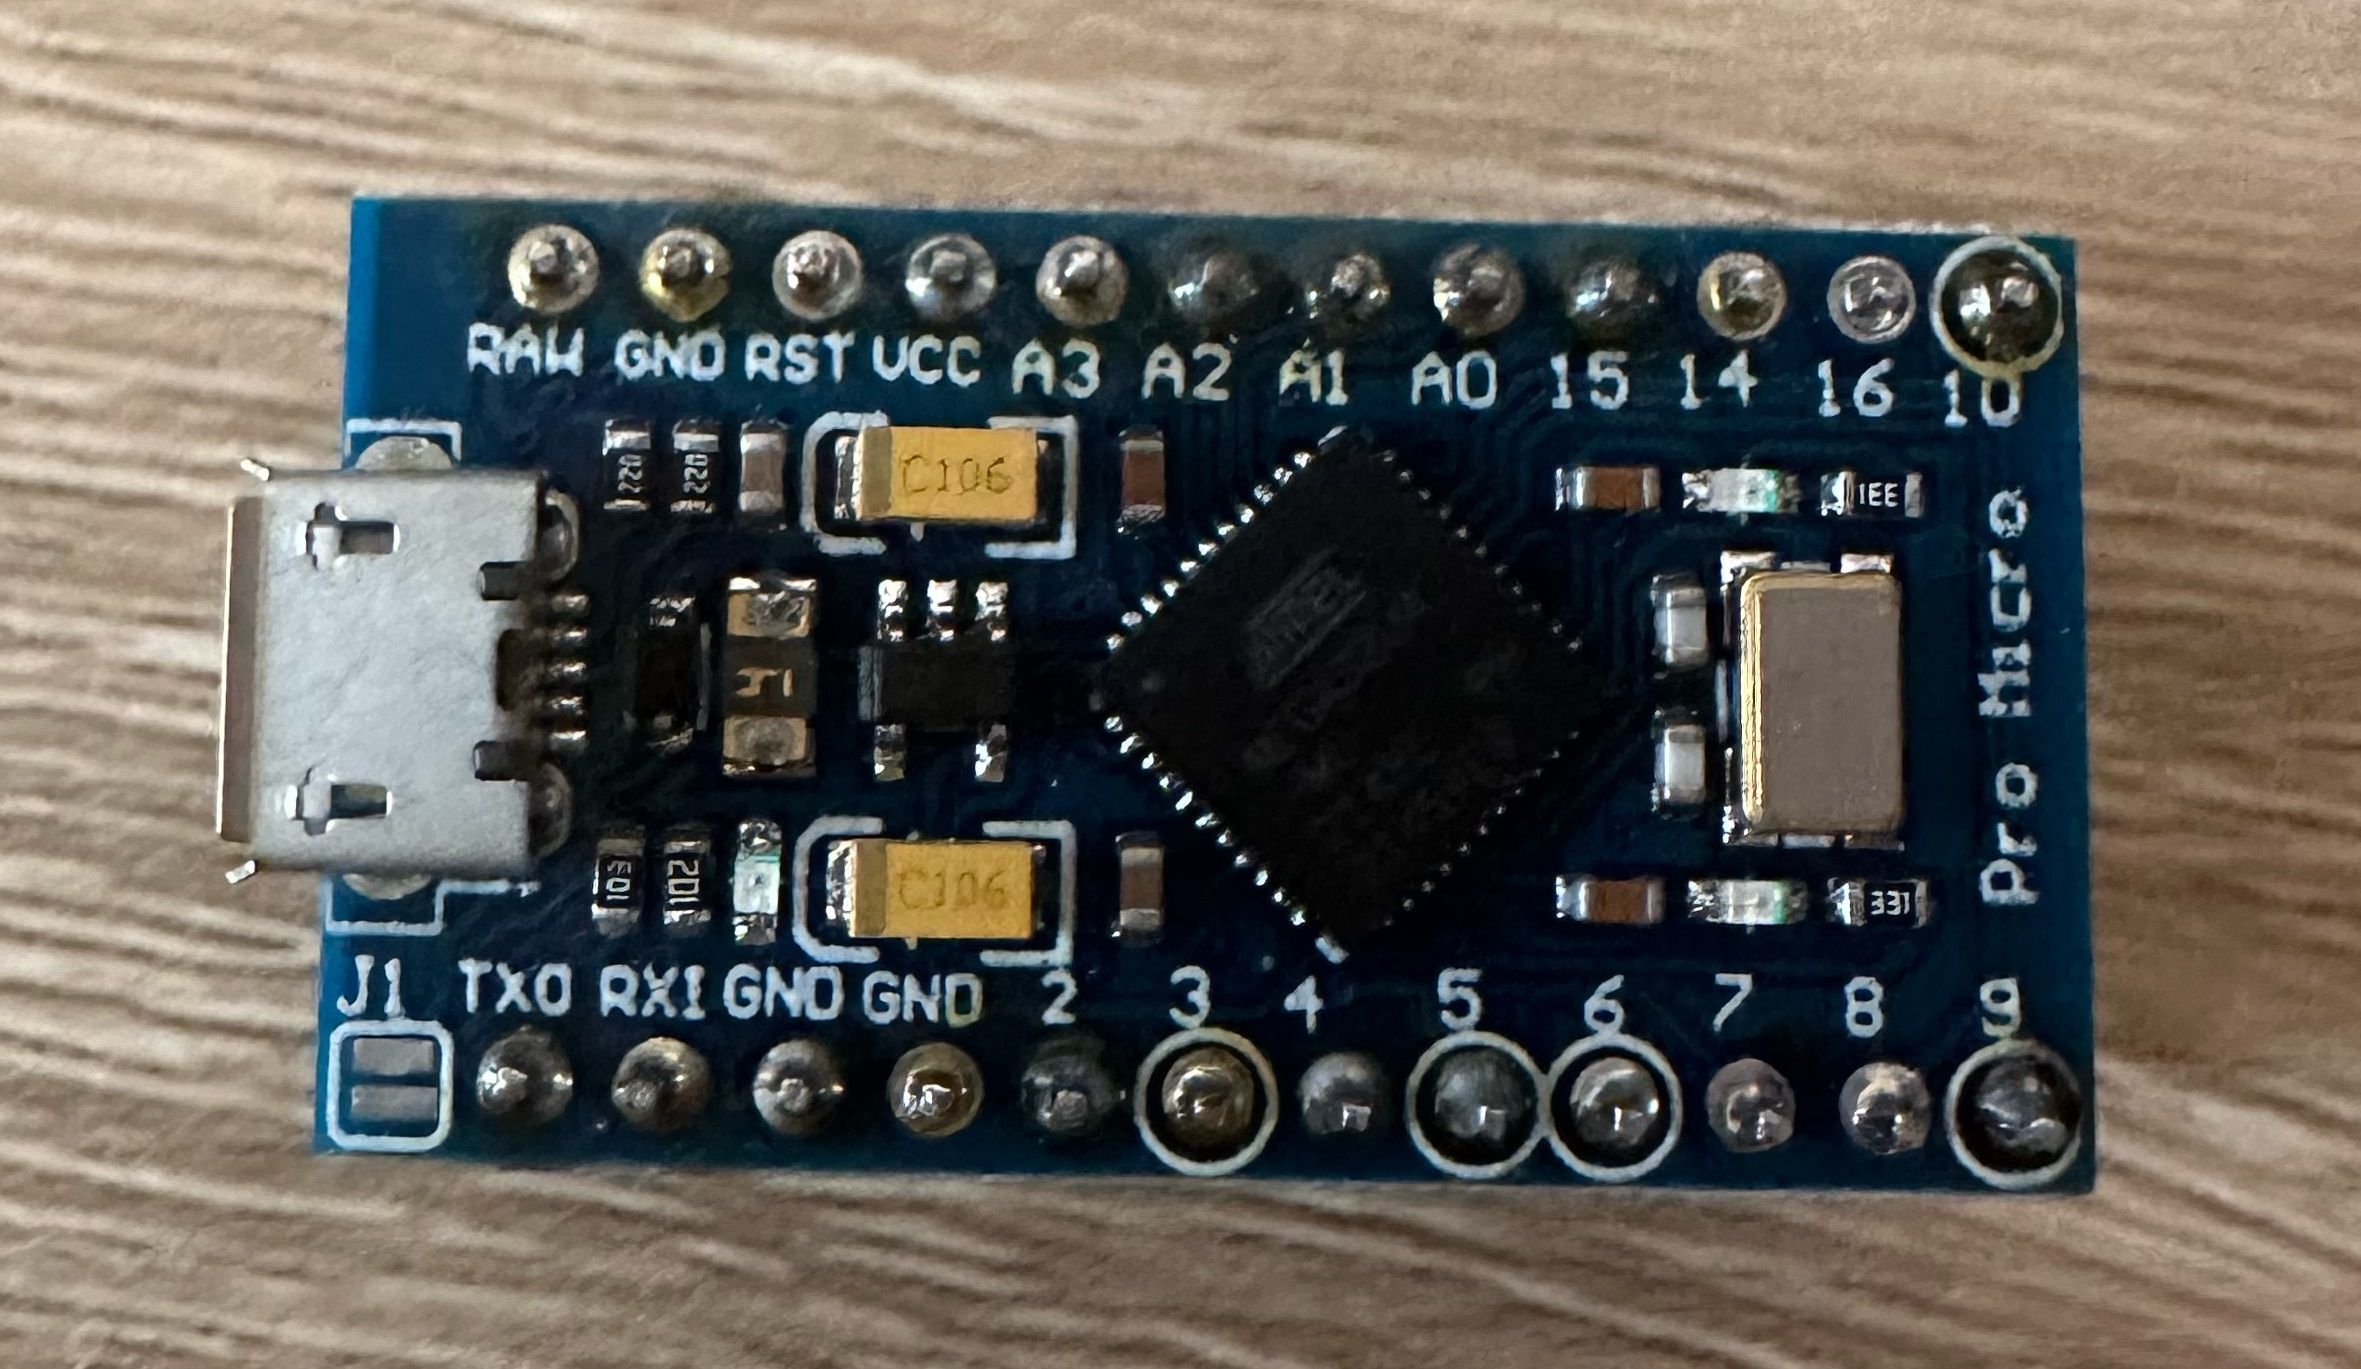
\includegraphics[width=0.45\textwidth]{imagenes/elemento-arduino.jpeg}}
            \label{fig:arduino_pro_micro}
            \subfigure[) Termistor LM35.]{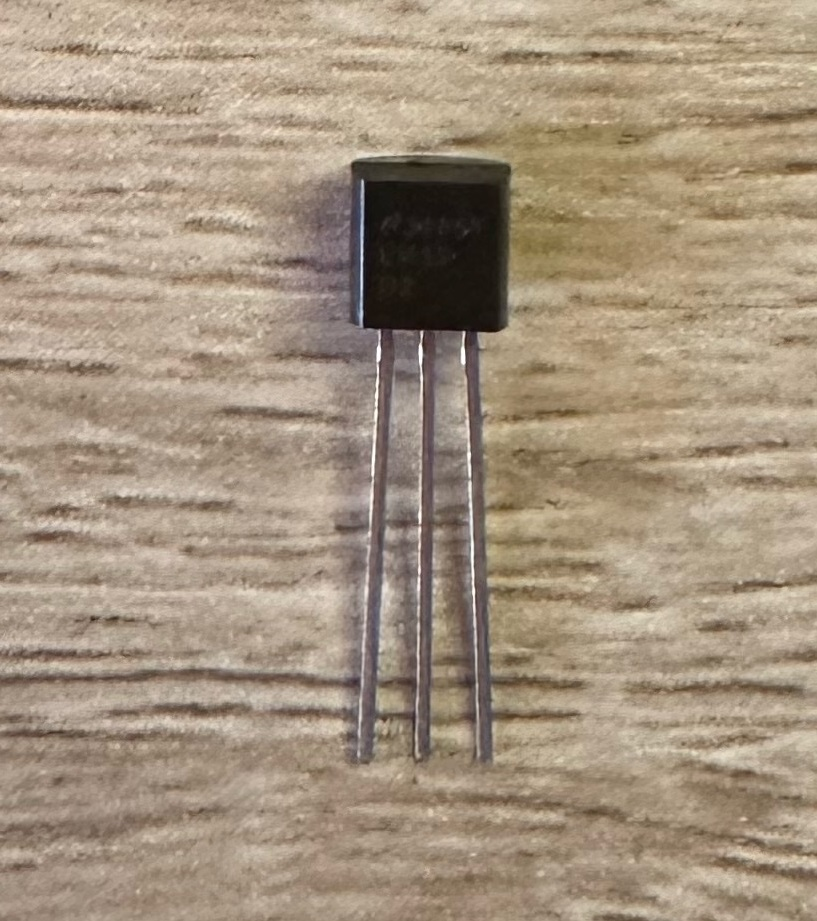
\includegraphics[width=0.3\textwidth, height=4.2cm]{imagenes/elemento-termistor.jpeg}}
            \label{fig:lm35_termistor}
        \end{minipage}
    \end{minipage}
\end{figure} 


\begin{figure}[H]
\begin{minipage}{\textwidth}
\centering
\begin{minipage}{\textwidth}
\centering
\subfigure[) GPS Neo-6M.]{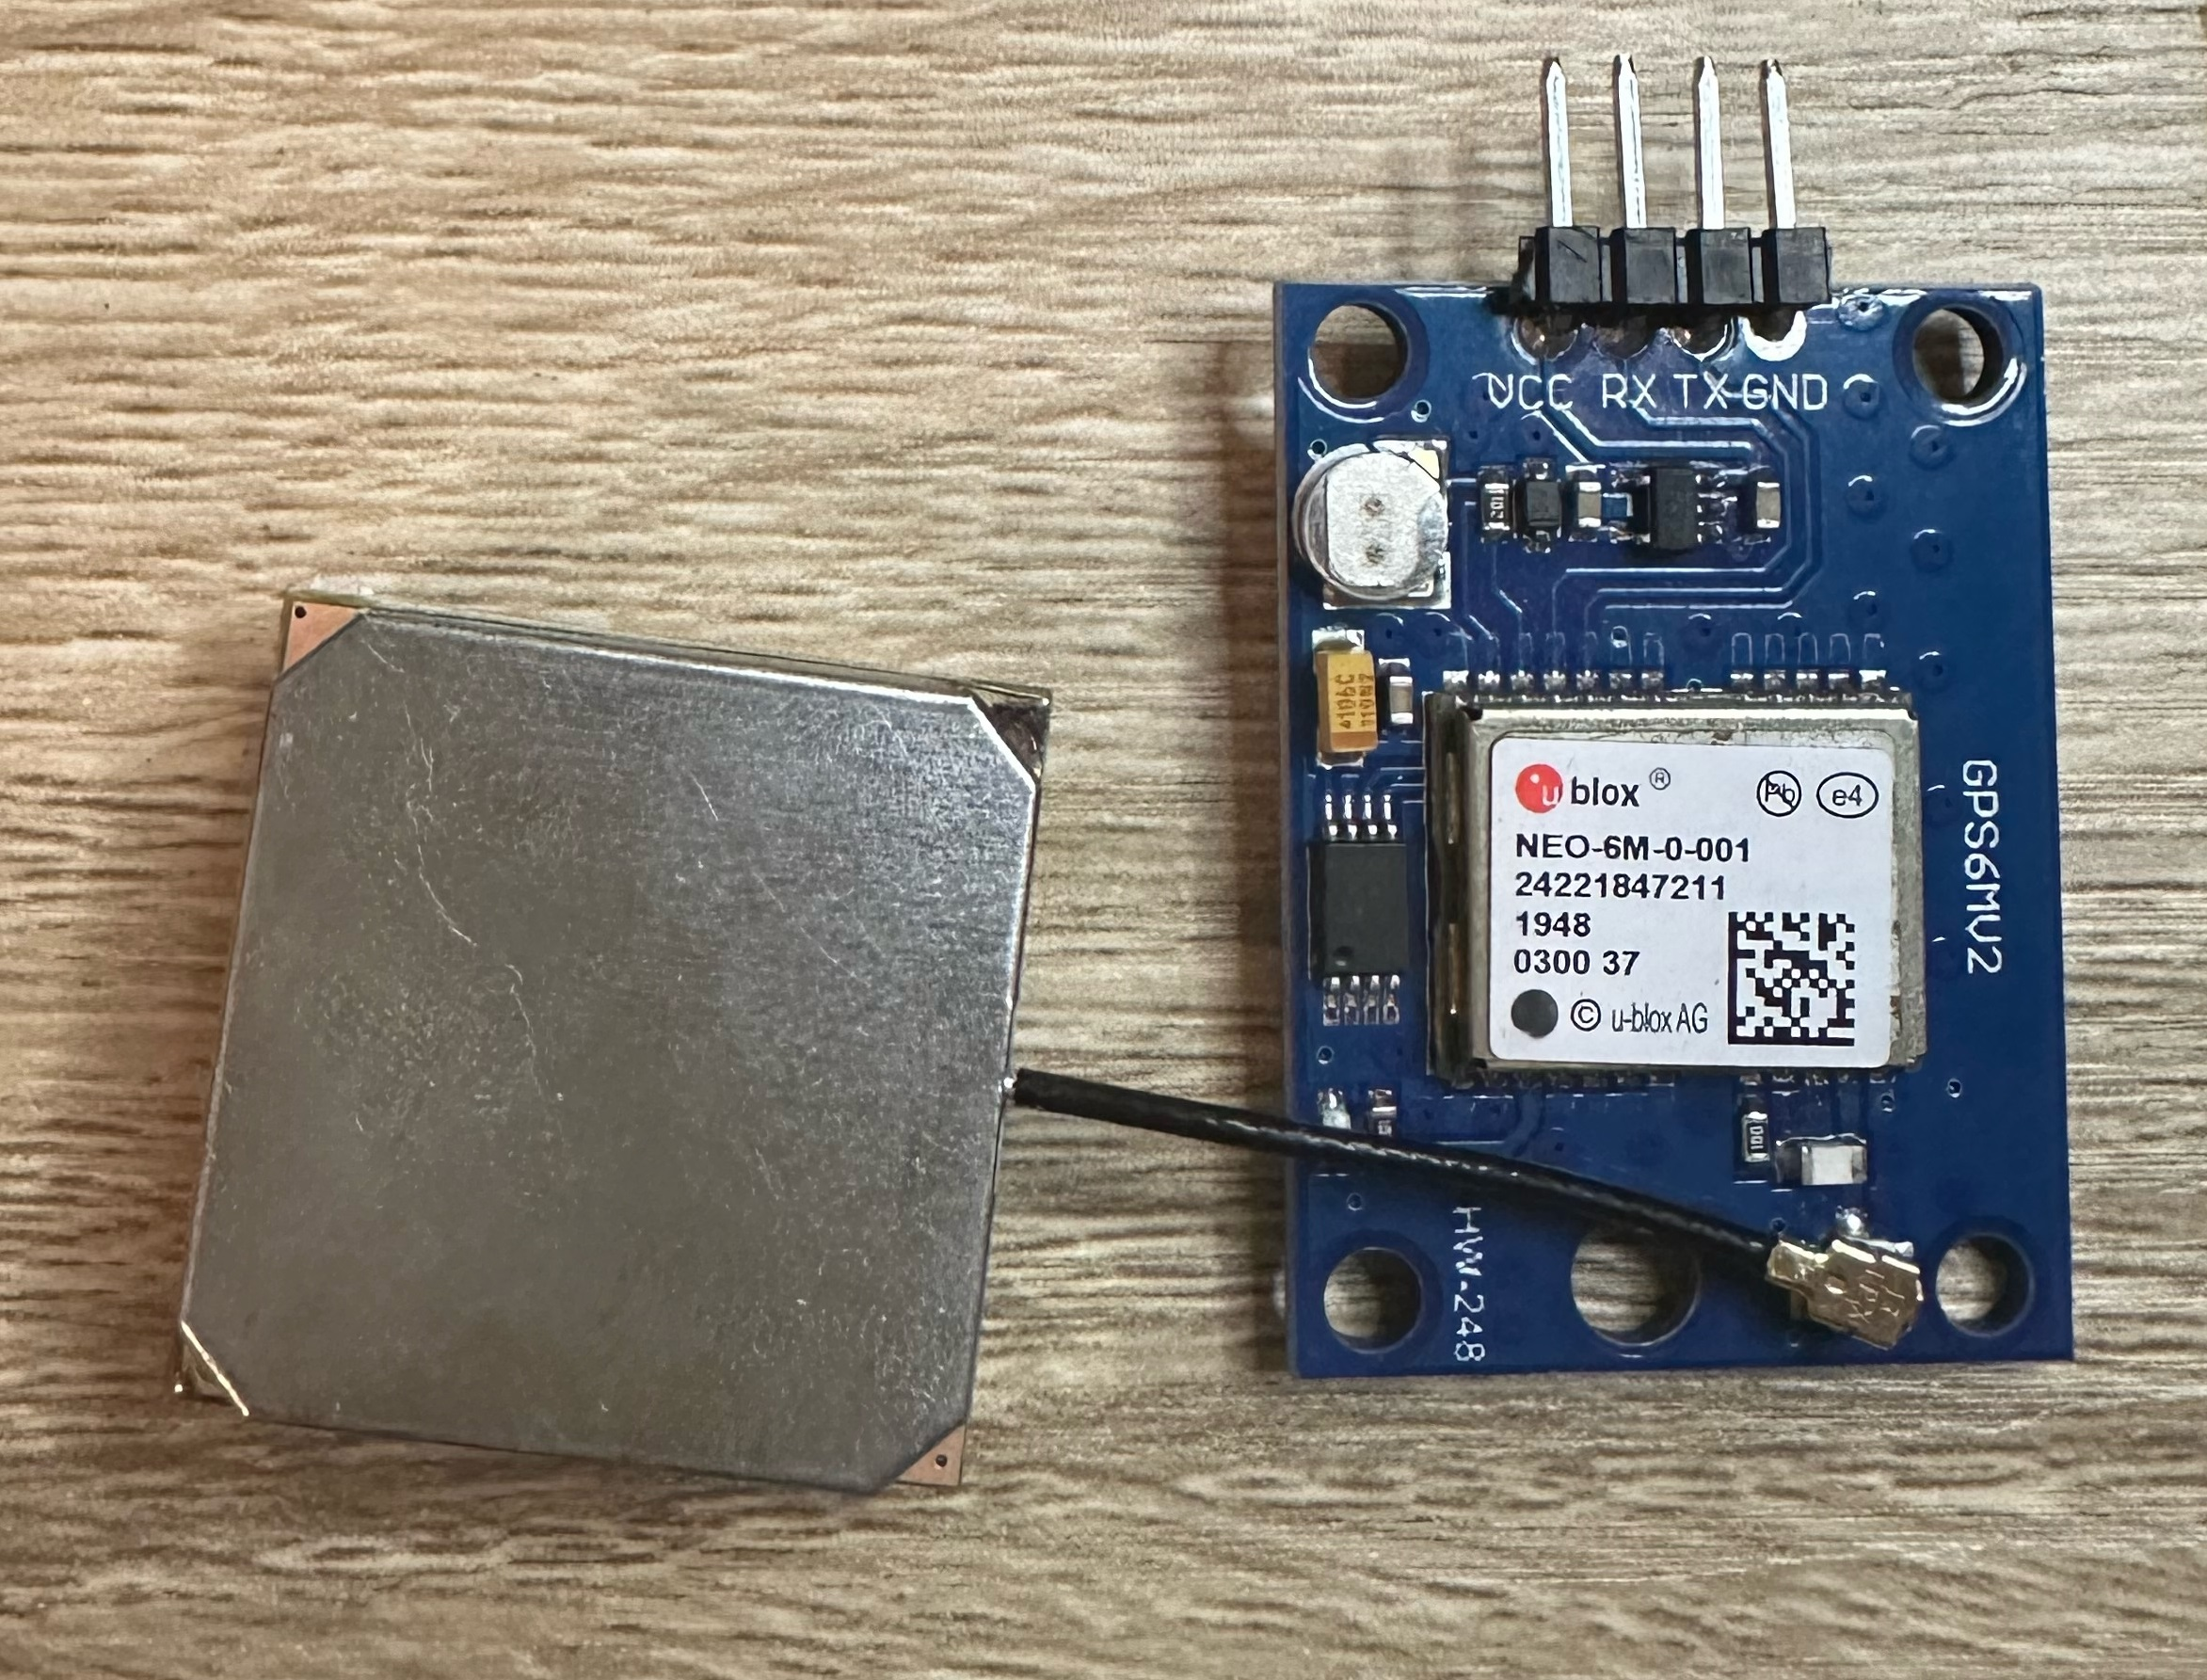
\includegraphics[ height=6cm]{imagenes/elemento-gps.jpeg}}
\label{fig
}
\subfigure[) Transceptor LoRa.]{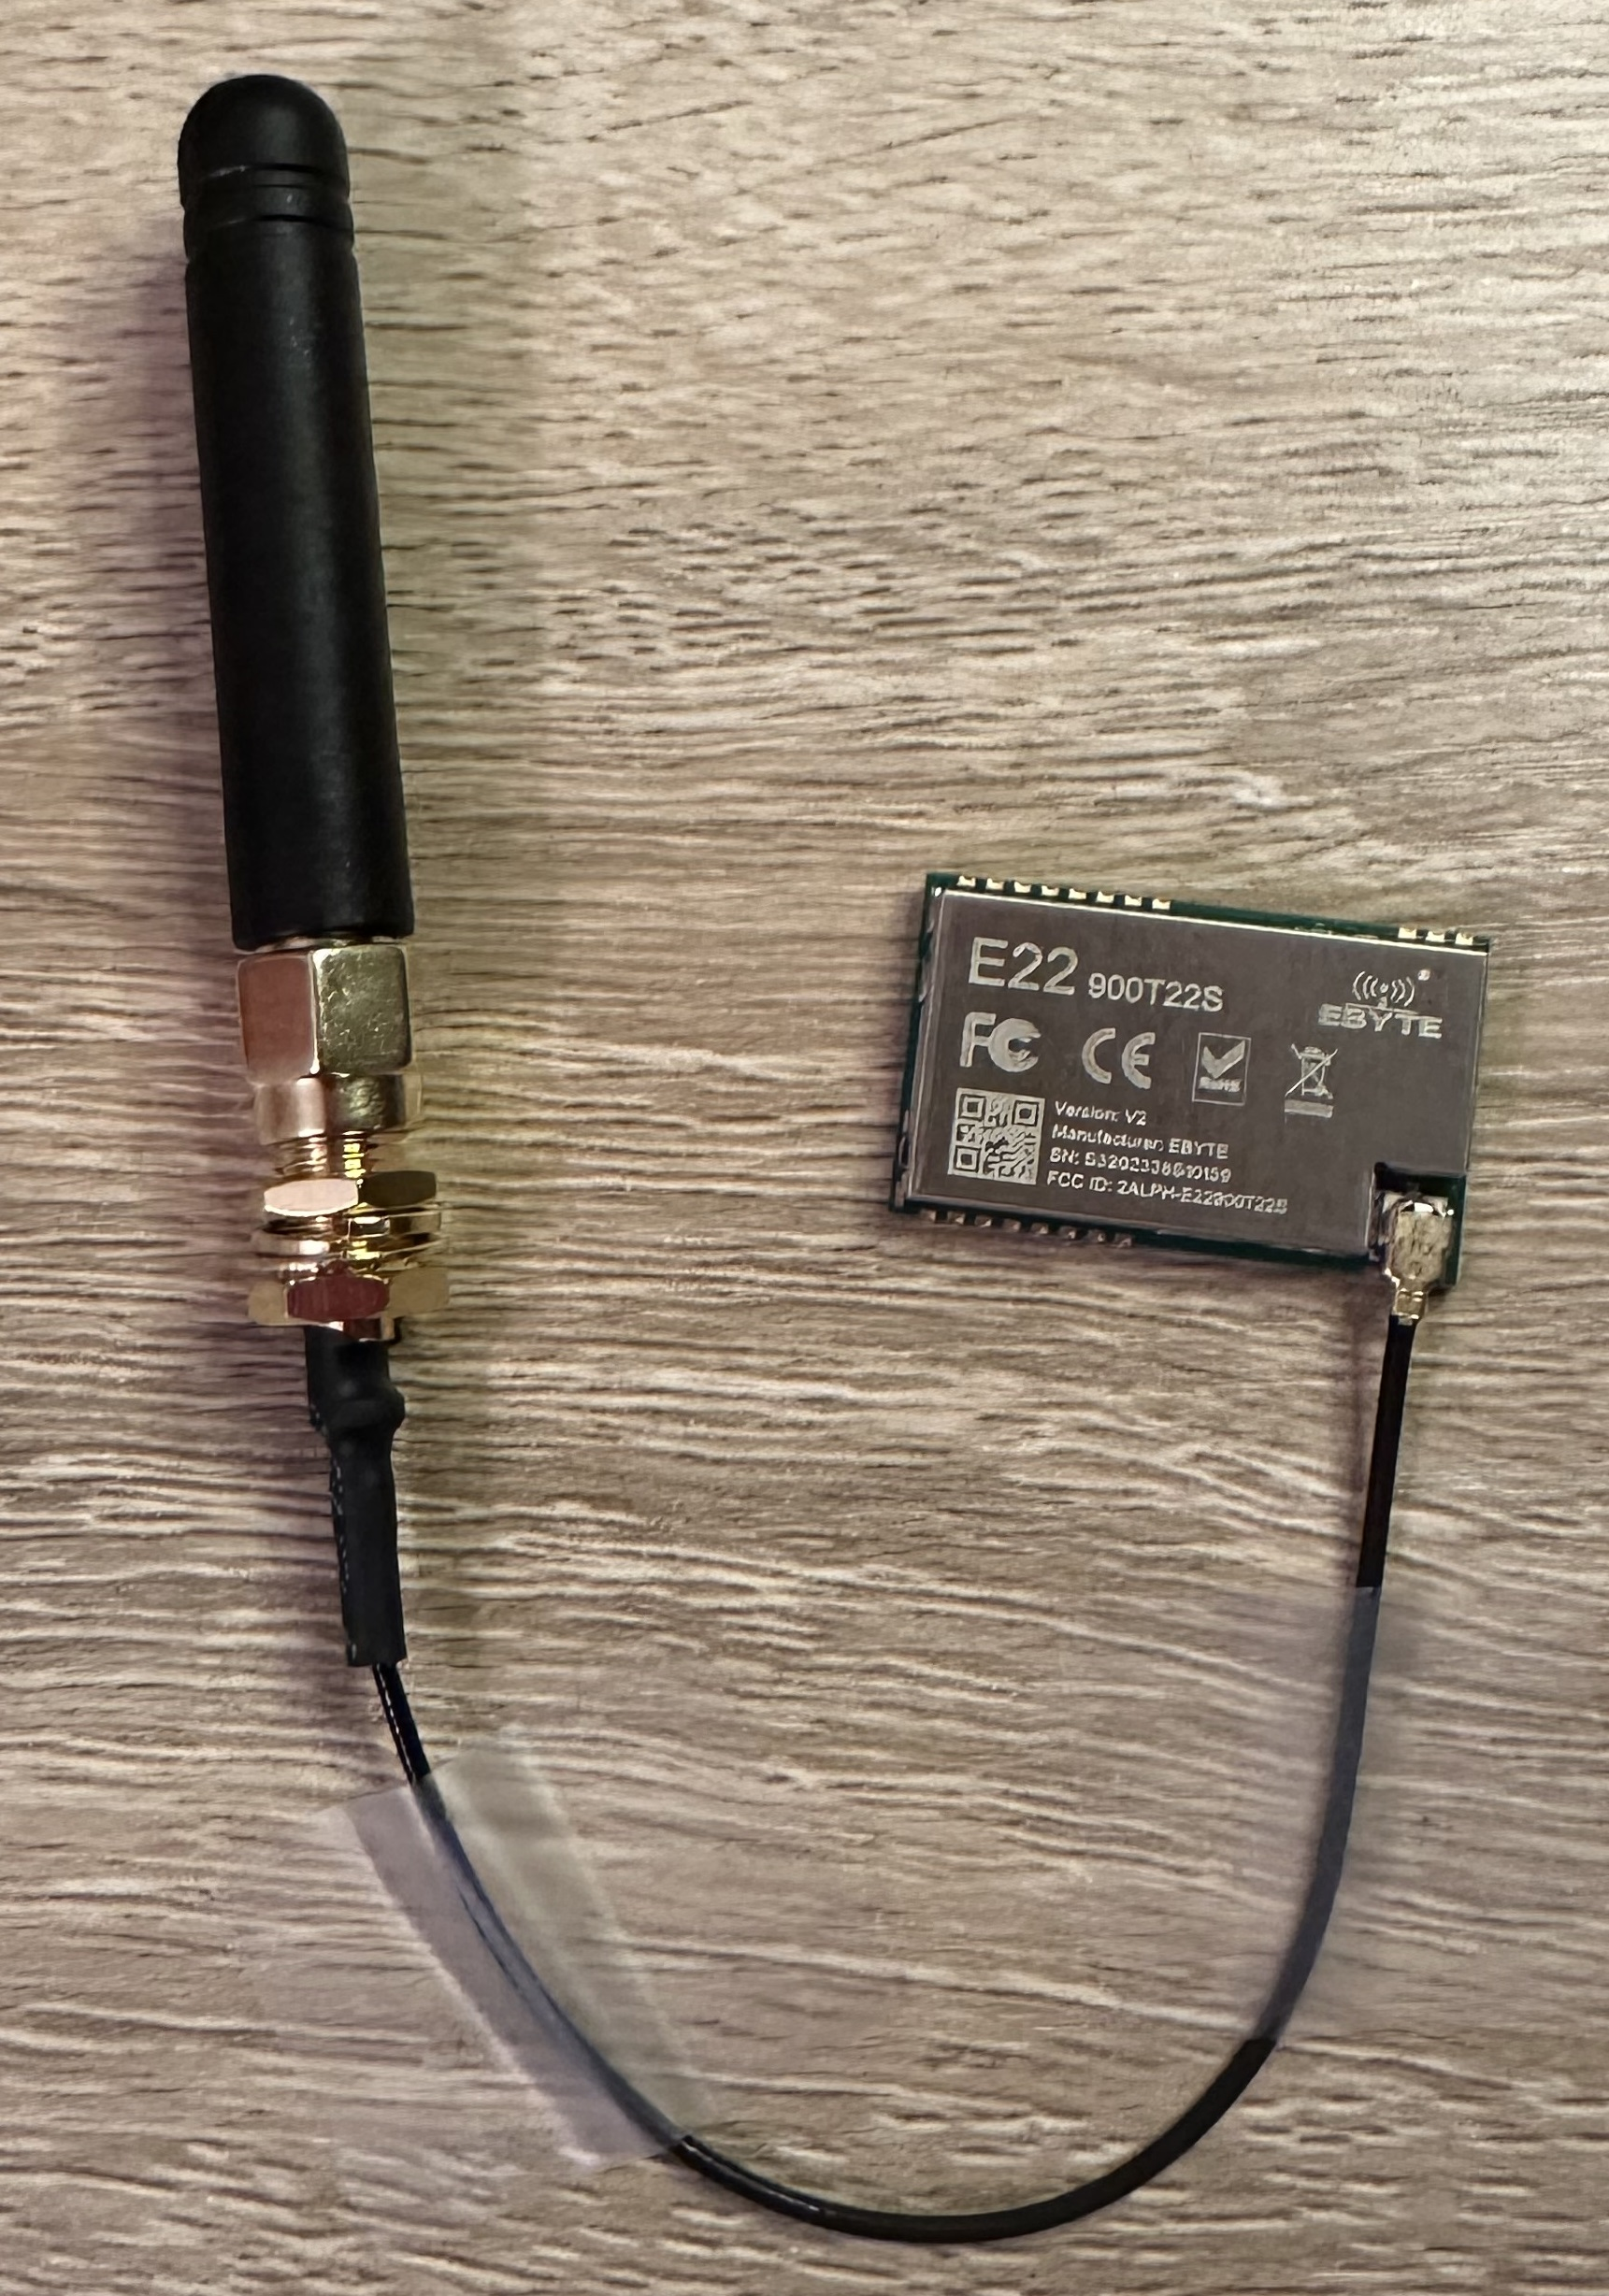
\includegraphics[ height=6cm]{imagenes/elemento-lora.jpg}}
\label{fig
}
\end{minipage}
\end{minipage}
    
    \begin{minipage}{\textwidth}
        \centering
        \begin{minipage}{\textwidth}
            \centering
            \subfigure[) Batería LiPo de 3.7V.]{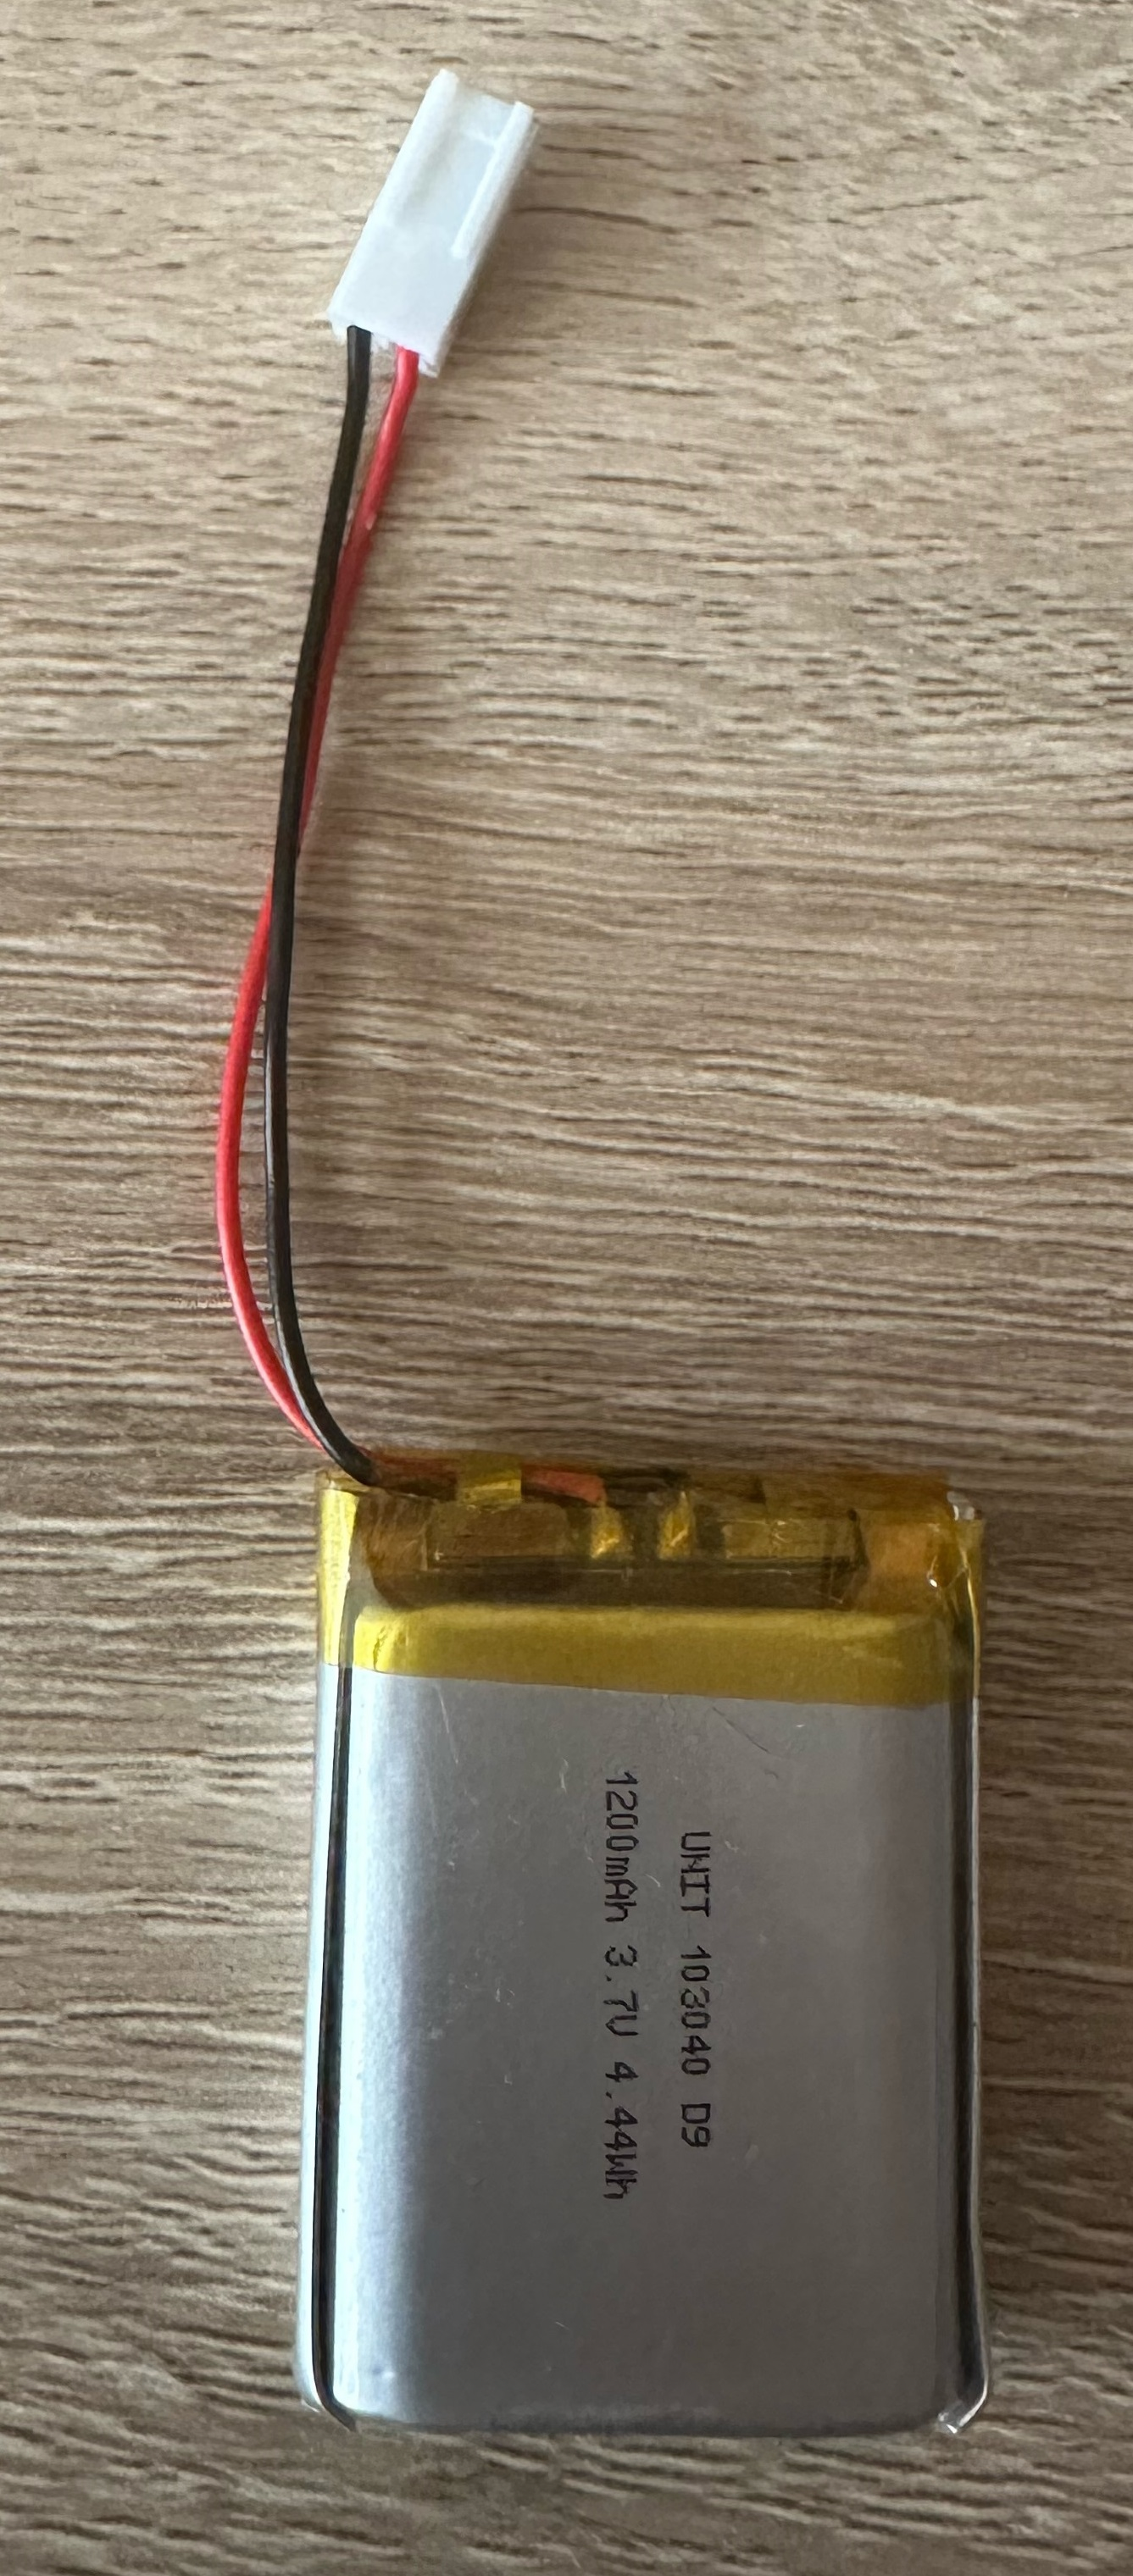
\includegraphics[ height=5cm]{imagenes/elemento-bateria.jpeg}}
            \label{fig:lipo_battery}
            \subfigure[) Cámara PR-700.]{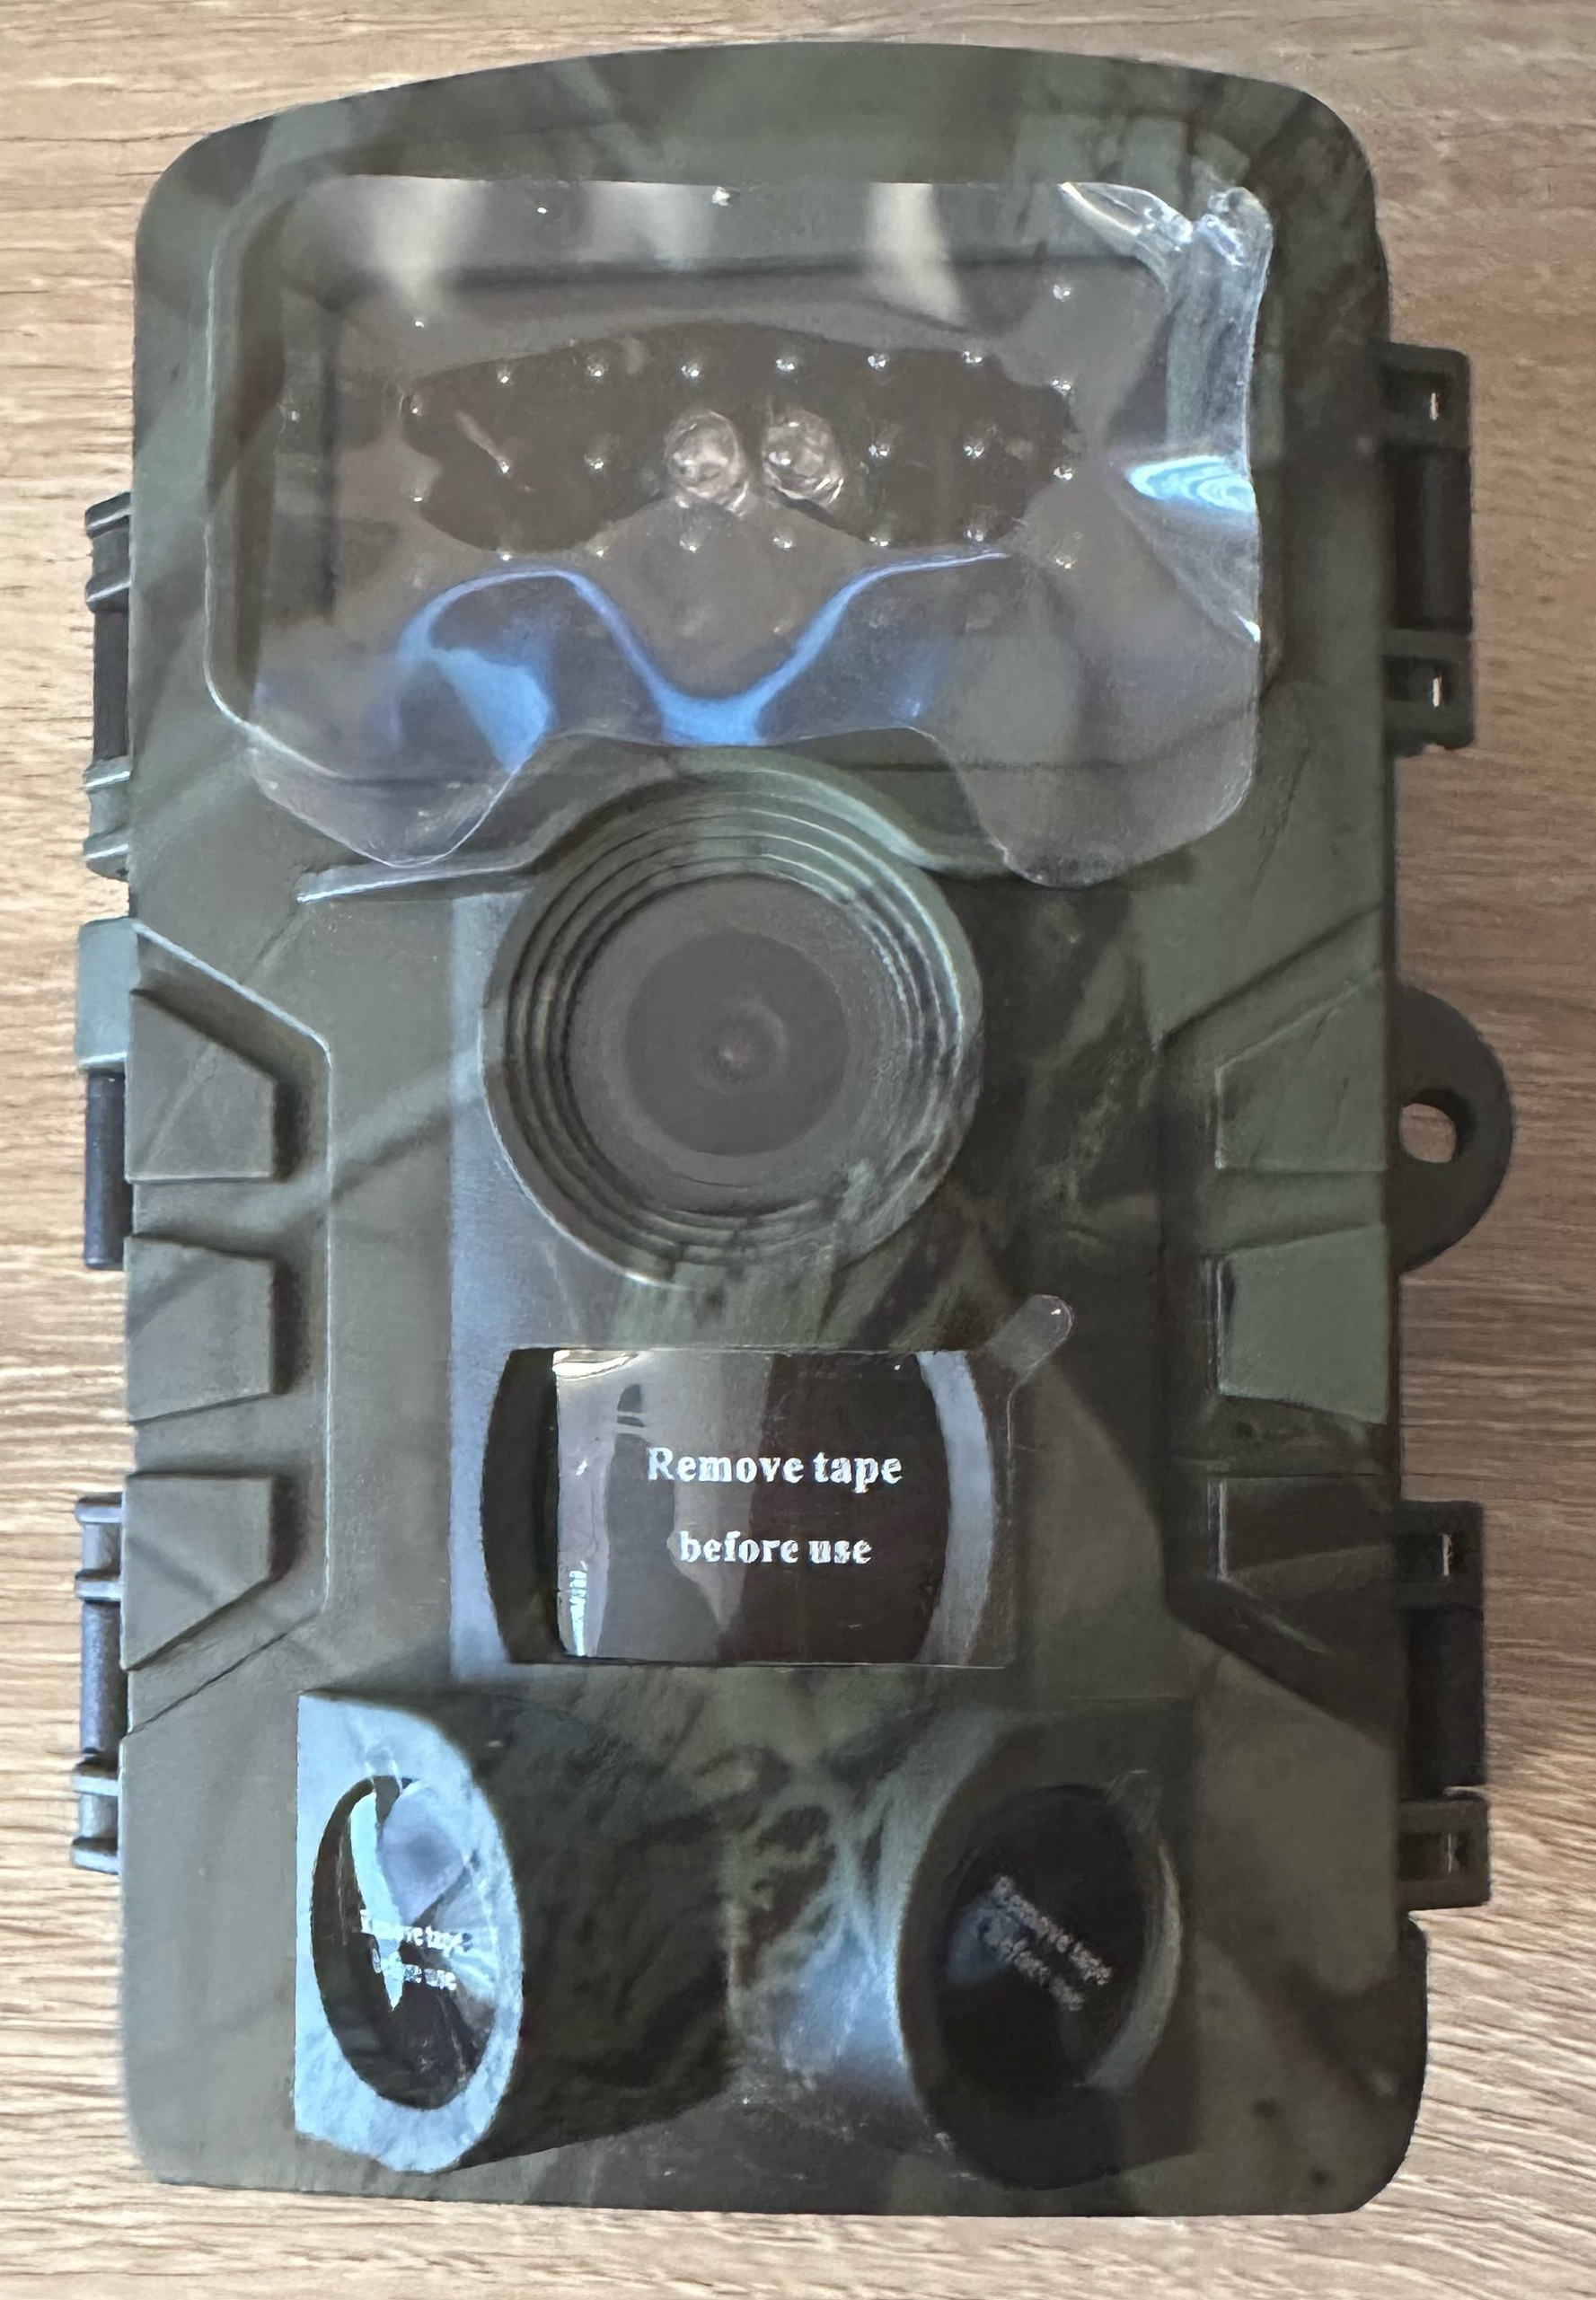
\includegraphics[ height=5cm]{imagenes/elemento-camara.jpeg}}
            \label{fig:pr_700_camera}
        \end{minipage}
    \end{minipage}
    
    \caption{Elementos adquiridos para la WSN.}
    \label{fig:wsn_elements}
\end{figure}


\subsection{Funcionamiento de los Elementos}
Una vez adquiridos todos los elementos necesarios para la implementación de la WSN, se verificará su funcionamiento. Esta etapa garantizará que cada componente funcione correctamente y esté listo para su integración en el sistema. A continuación, se describen los pasos para verificar el funcionamiento de cada elemento:
\begin{itemize}
    \item \textbf{Arduino Pro Micro:}
    
Se conecta el Arduino Pro Micro a un puerto USB disponible en el ordenador mediante un cable USB adecuado y se verifica que el LED de alimentación del Arduino Pro Micro se encienda, lo que indica que está recibiendo energía correctamente.

Se carga un programa de prueba simple en el Arduino Pro Micro utilizando el entorno de desarrollo Arduino IDE. Este programa puede ser tan básico como hacer parpadear el LED interno del Arduino cada segundo.

Se observa el comportamiento del Arduino Pro Micro para confirmar que responde correctamente al programa cargado. Se espera que el LED conectado parpadee según lo programado, lo que indica que el Arduino está funcionando correctamente.
\begin{figure}[H]
    \centering
    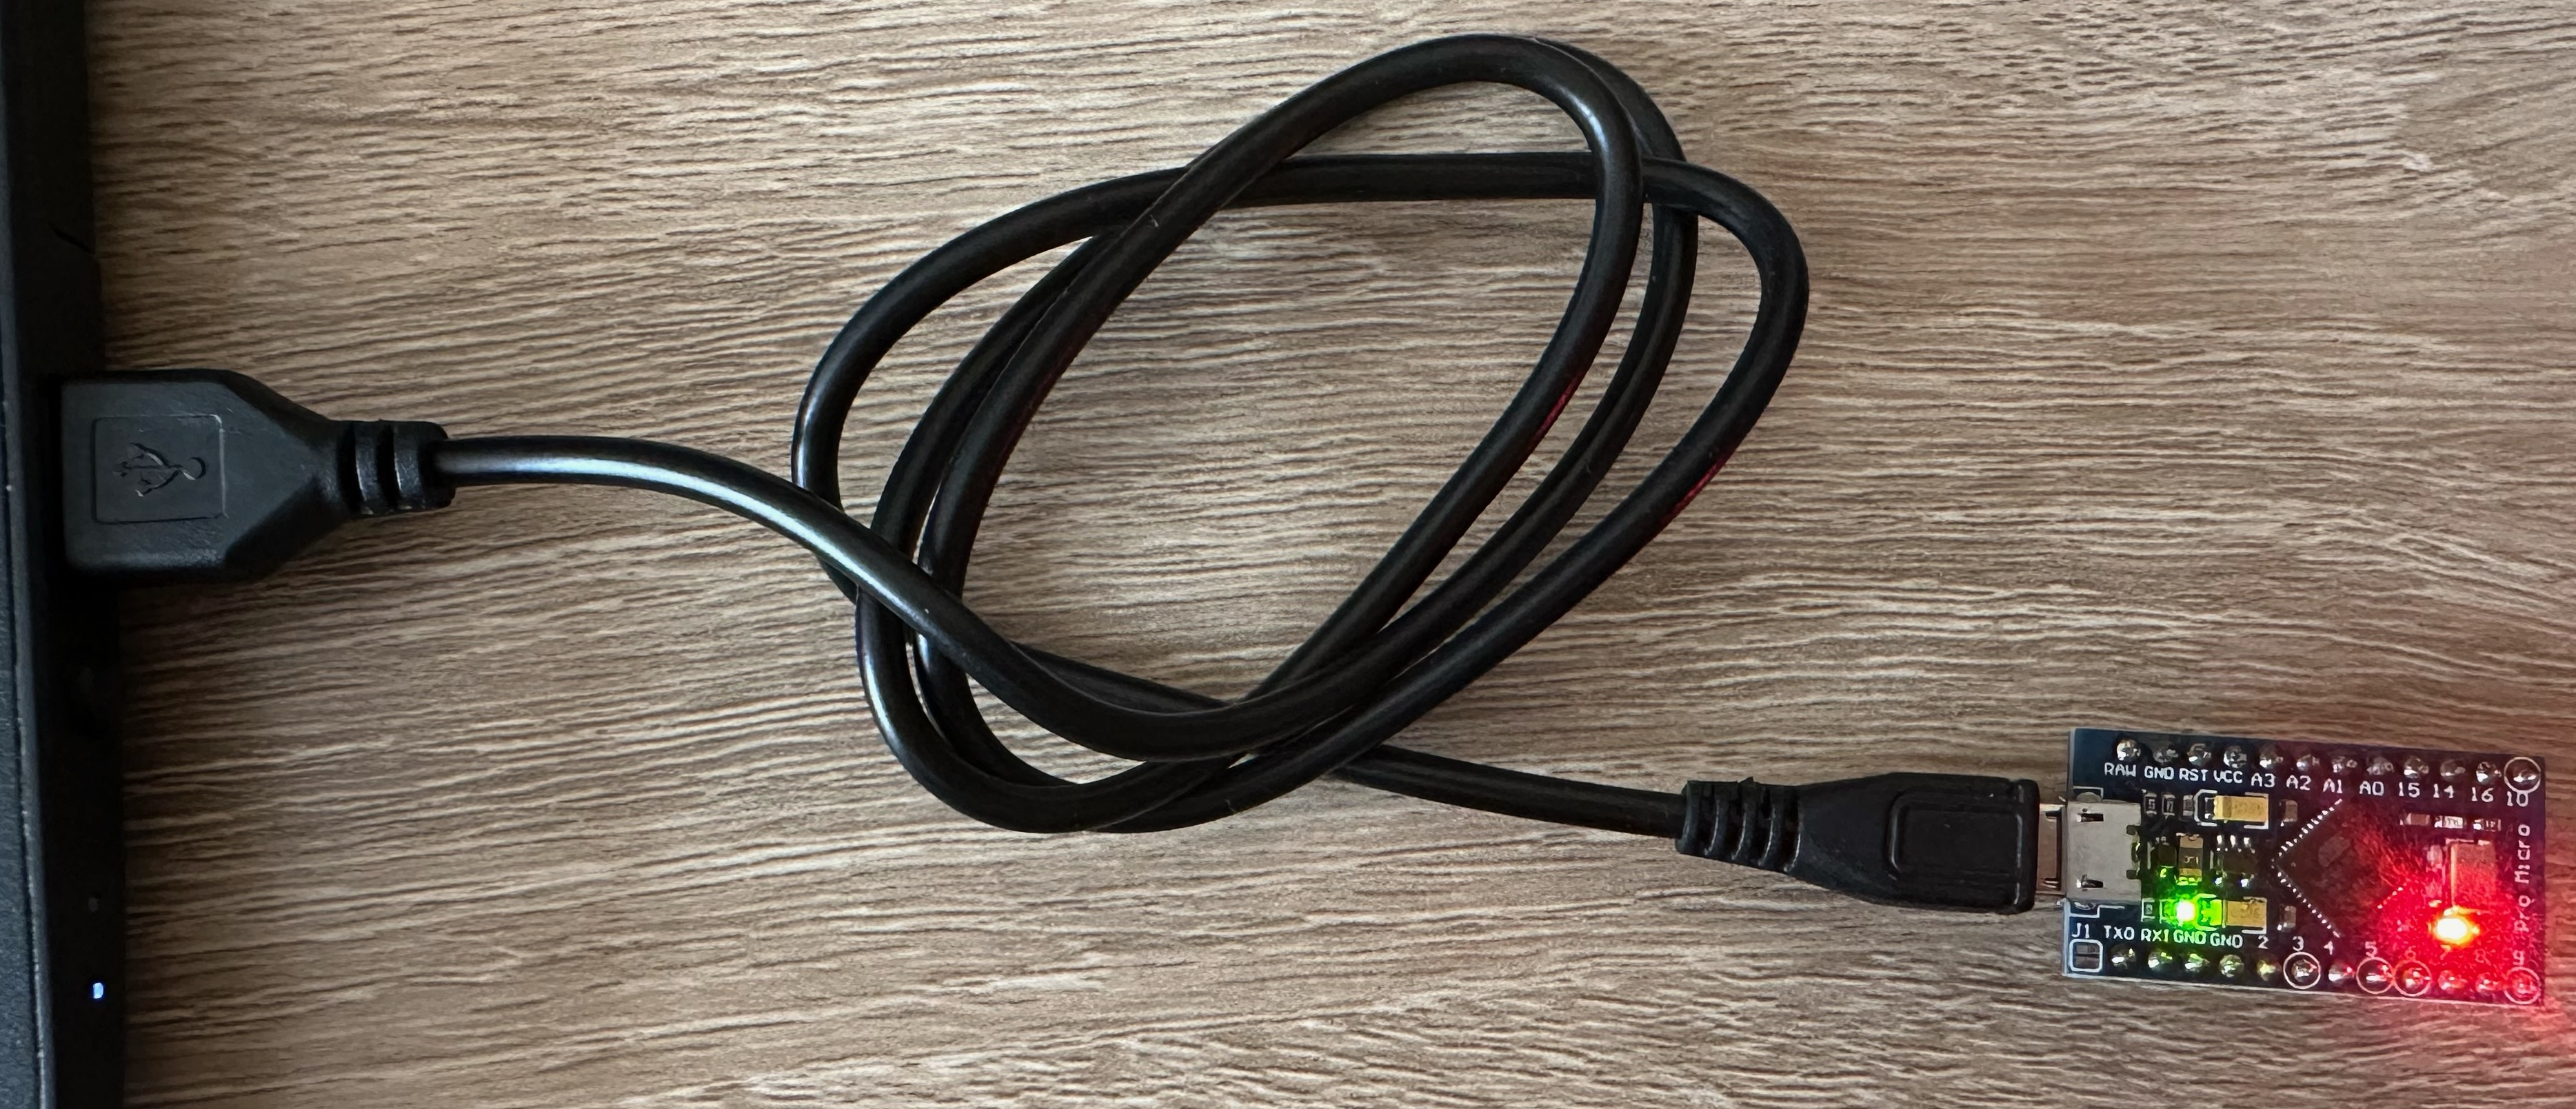
\includegraphics[width=0.6\textwidth]{imagenes/prueba-led.jpeg}
    \caption{Prueba del led interno de Arduino Pro Micro.}
    \label{fig:prueba_led_arduino}
\end{figure}

\item \textbf{Termistor LM35:}

El termistor LM35 se conecta a la placa Arduino según las especificaciones del fabricante. Se conecta el pin de salida del termistor al pin analógico de lectura de la placa Arduino (por ejemplo, A0), el pin VCC del termistor al pin de 5V de la placa Arduino, y el pin GND del termistor al pin de tierra (GND) de la placa Arduino.

Para probar su funcionamiento, se desarrolla un programa en el entorno de desarrollo Arduino IDE para leer la temperatura ambiente mediante el termistor LM35. Este programa realiza la lectura del valor analógico del pin conectado al termistor y lo convierte a temperatura en grados Celsius utilizando la fórmula proporcionada por el datasheet del LM35, la cual es: $\text{T[°C]} = \left( \frac{\text{valorSensor} \times 5}{1023} \right) \times 100$ .  

Una vez cargado el programa en la placa Arduino, se puede verificar la correcta lectura de la temperatura ambiente. Si se coloca el termistor en un entorno con una temperatura conocida y se observa la salida del monitor serial en el Arduino IDE. Se pueden comparar las lecturas obtenidas con la temperatura ambiente medida independientemente para verificar la precisión del termistor en la medición de la temperatura.

\begin{figure}[H]
    \centering
    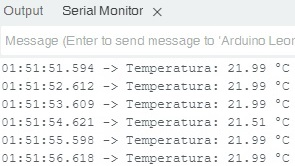
\includegraphics[width=0.5\textwidth, height=4cm]{imagenes/temperatura_solo.jpg}
    \caption{Resultado de registrar la temperatura del termistor LM35.}
    \label{fig:temp-solo}
\end{figure}

\begin{figure}[H]
    \centering
    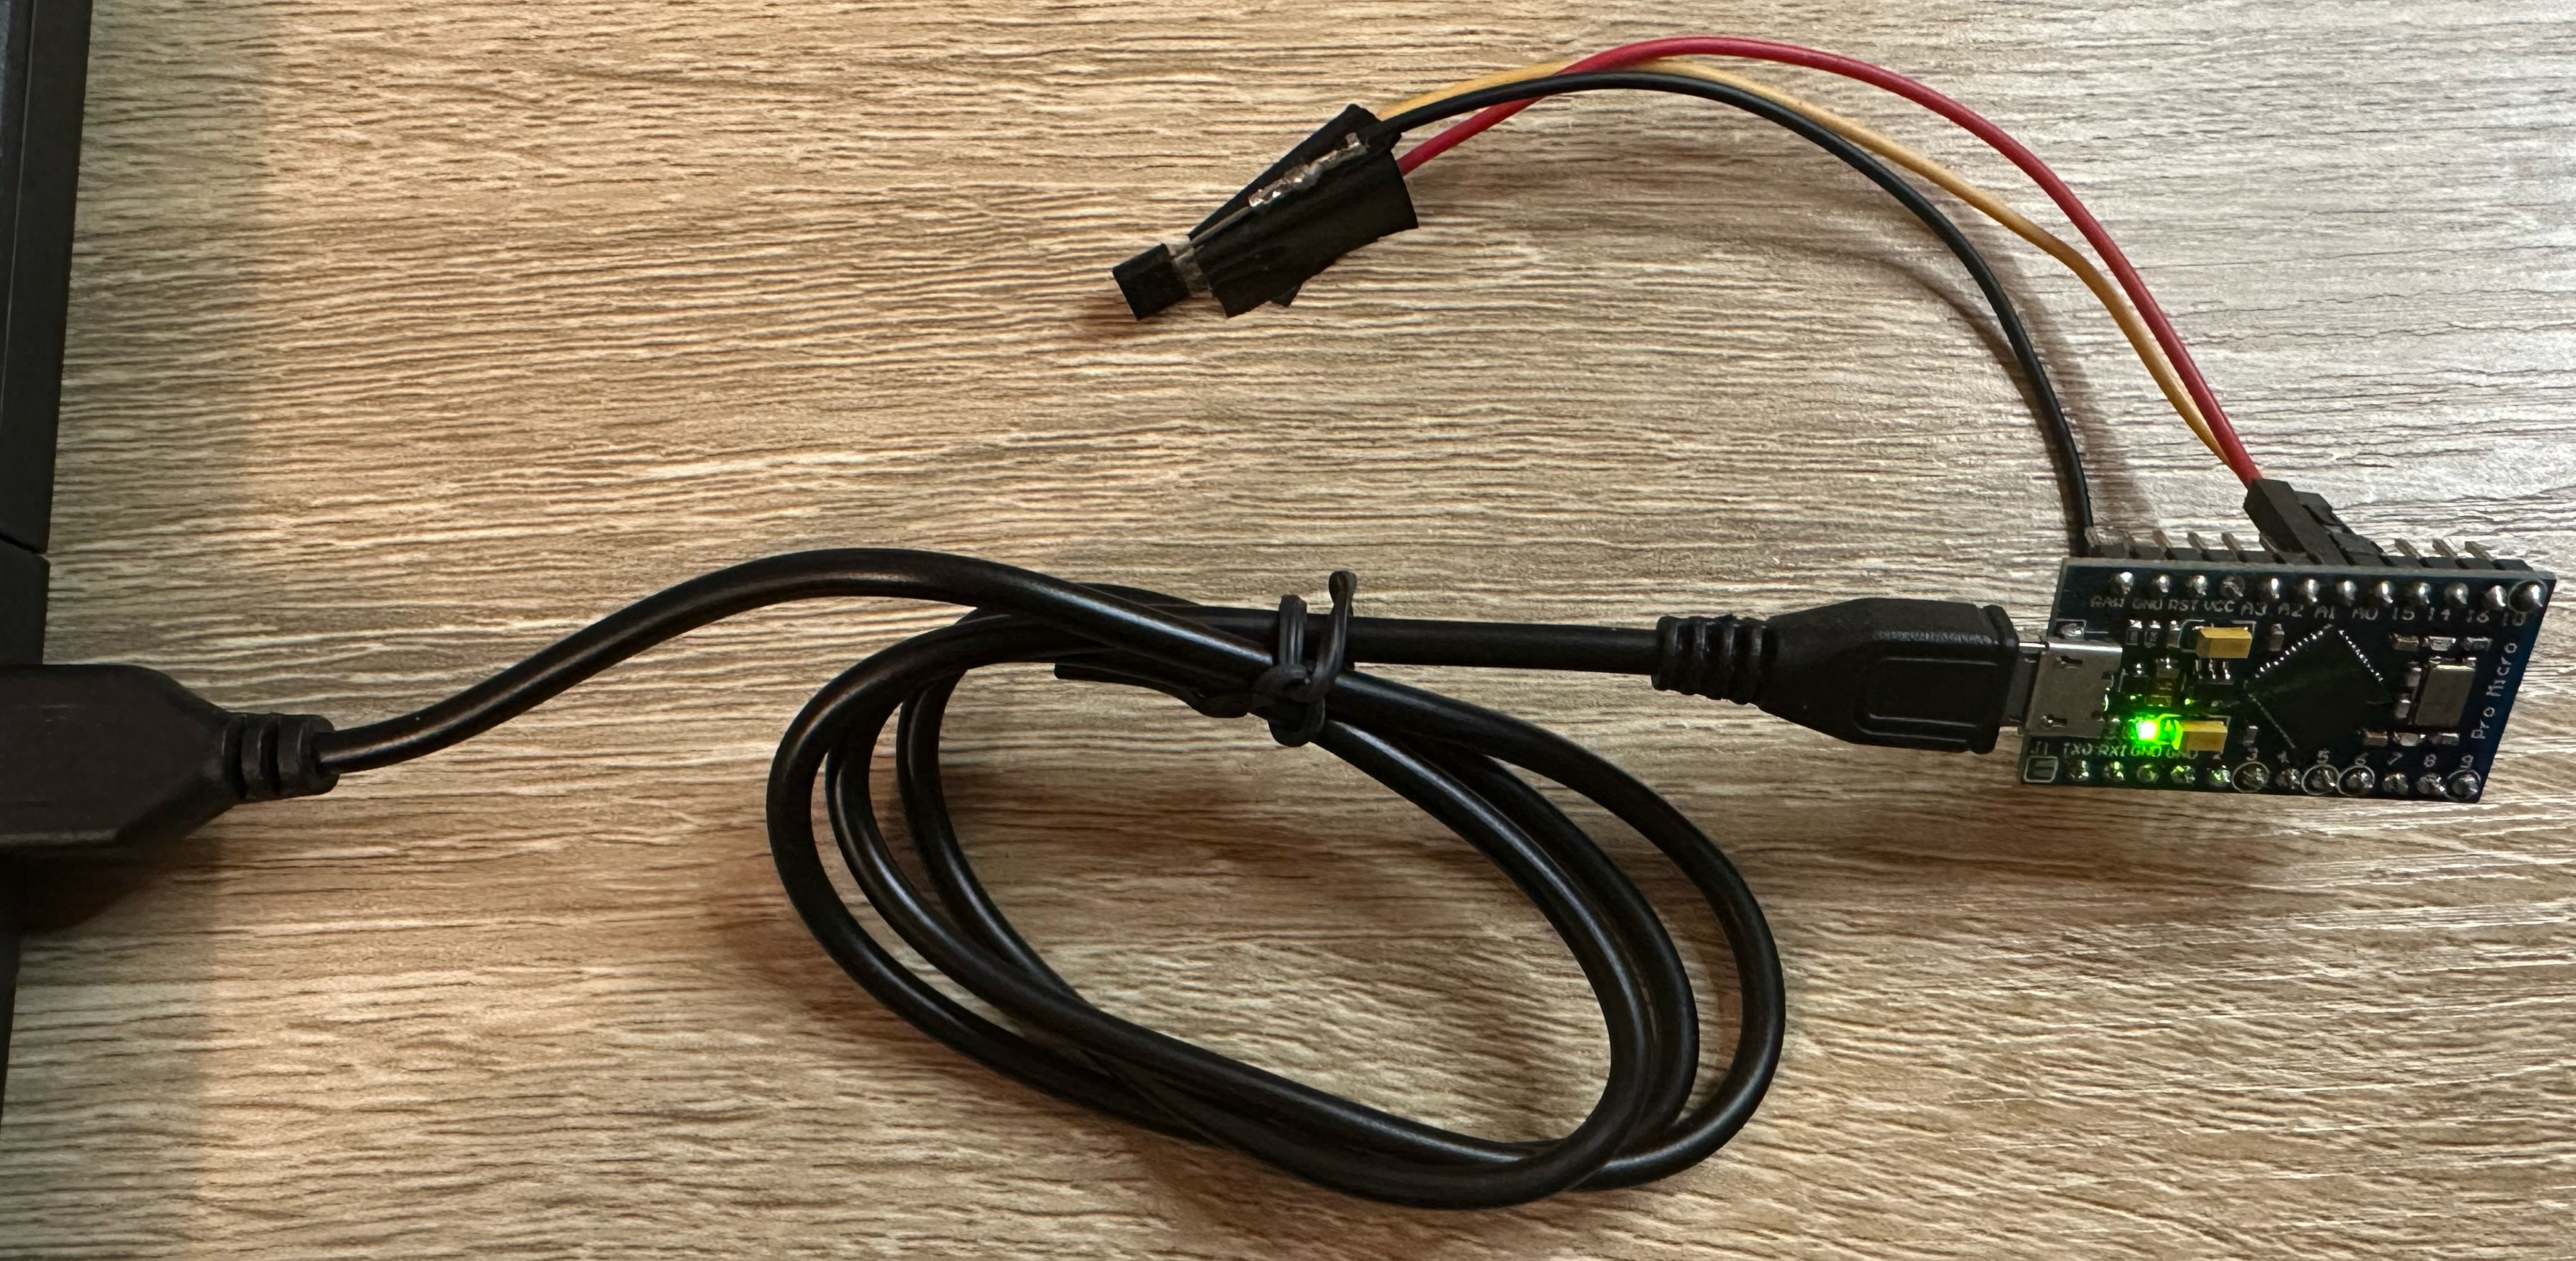
\includegraphics[width=0.6\textwidth, height=4cm]{imagenes/prueba-termistor.jpeg}
    \caption{Prueba del termistor LM35 usando el Arduino Pro Micro.}
    \label{fig:prueba_termistor}
\end{figure}


\item \textbf{Módulo GPS Neo-6M:}

El módulo GPS Neo-6M se conecta a la placa Arduino siguiendo las especificaciones proporcionadas por el fabricante. Se conecta el pin de datos del módulo GPS (RX) al pin TX de la placa Arduino y el pin de datos (TX) al pin RX de la placa Arduino mediante cables jumper. De igual modo, se conectan los pines VCC y GND del módulo GPS a los pines de alimentación de 5V (VCC) y tierra (GND) de la placa Arduino, respectivamente.

Se desarrolla un programa en el entorno de desarrollo Arduino IDE para configurar el módulo GPS Neo-6M y recibir datos de los satélites para obtener la ubicación actual. El programa establece la comunicación serial con el módulo GPS y envía los comandos AT necesarios para configurar el módulo y solicitar datos de ubicación.

Para la realización de este programa, primeramente se desarrolló y probó en una placa Arduino Uno, utilizando la librería TinyGPS++, esto debido a que se presentaban problemas de comunicación al utilizarlo con un Arduino Pro Micro. Una vez verificado que el programa funcione correctamente en la placa Arduino Uno, que el módulo GPS adquiera señales de satélite y que proporcione datos precisos de ubicación, se procedió a ajustar la velocidad de comunicación del módulo para que fuera compatible con el Arduino Pro Micro.

Esto mediante un nuevo programa encargado de configurar la velocidad de comunicación del módulo GPS Neo-6M a través del envío de un comando específico (\$PMTK251,9600*17). Luego, en el bucle principal, se lee la información proporcionada por el módulo GPS y se procesa el mensaje GPRMC para obtener la latitud, la longitud y la hora.

Las coordenadas obtenidas se convierten a formato decimal y se ajustan según el hemisferio y el huso horario para obtener la ubicación exacta y la hora local de la Ciudad de México (GMT-6). Finalmente, se imprimen las coordenadas y la hora en el formato deseado.

Una vez cargado el programa en la placa Arduino, se procede a verificar que el módulo GPS pueda adquirir señales de satélite y proporcionar datos precisos de ubicación. Se coloca el módulo GPS en un lugar abierto y se observa la salida del monitor serial en el Arduino IDE. Se verifican los datos de ubicación proporcionados por el módulo GPS y se comparan con la ubicación conocida para asegurar su precisión.

\begin{figure}[H]
    \centering
    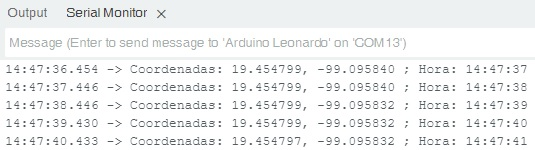
\includegraphics[width=0.75\textwidth, height=4cm]{imagenes/gps_solo.jpg}
    \caption{Resultado de obtener las coordenadas y la hora mediante el GPS-6M.}
    \label{fig:gps-solo}
\end{figure}

\begin{figure}[H]
    \centering
    \subfigure[) Usando el Arduino UNO.]{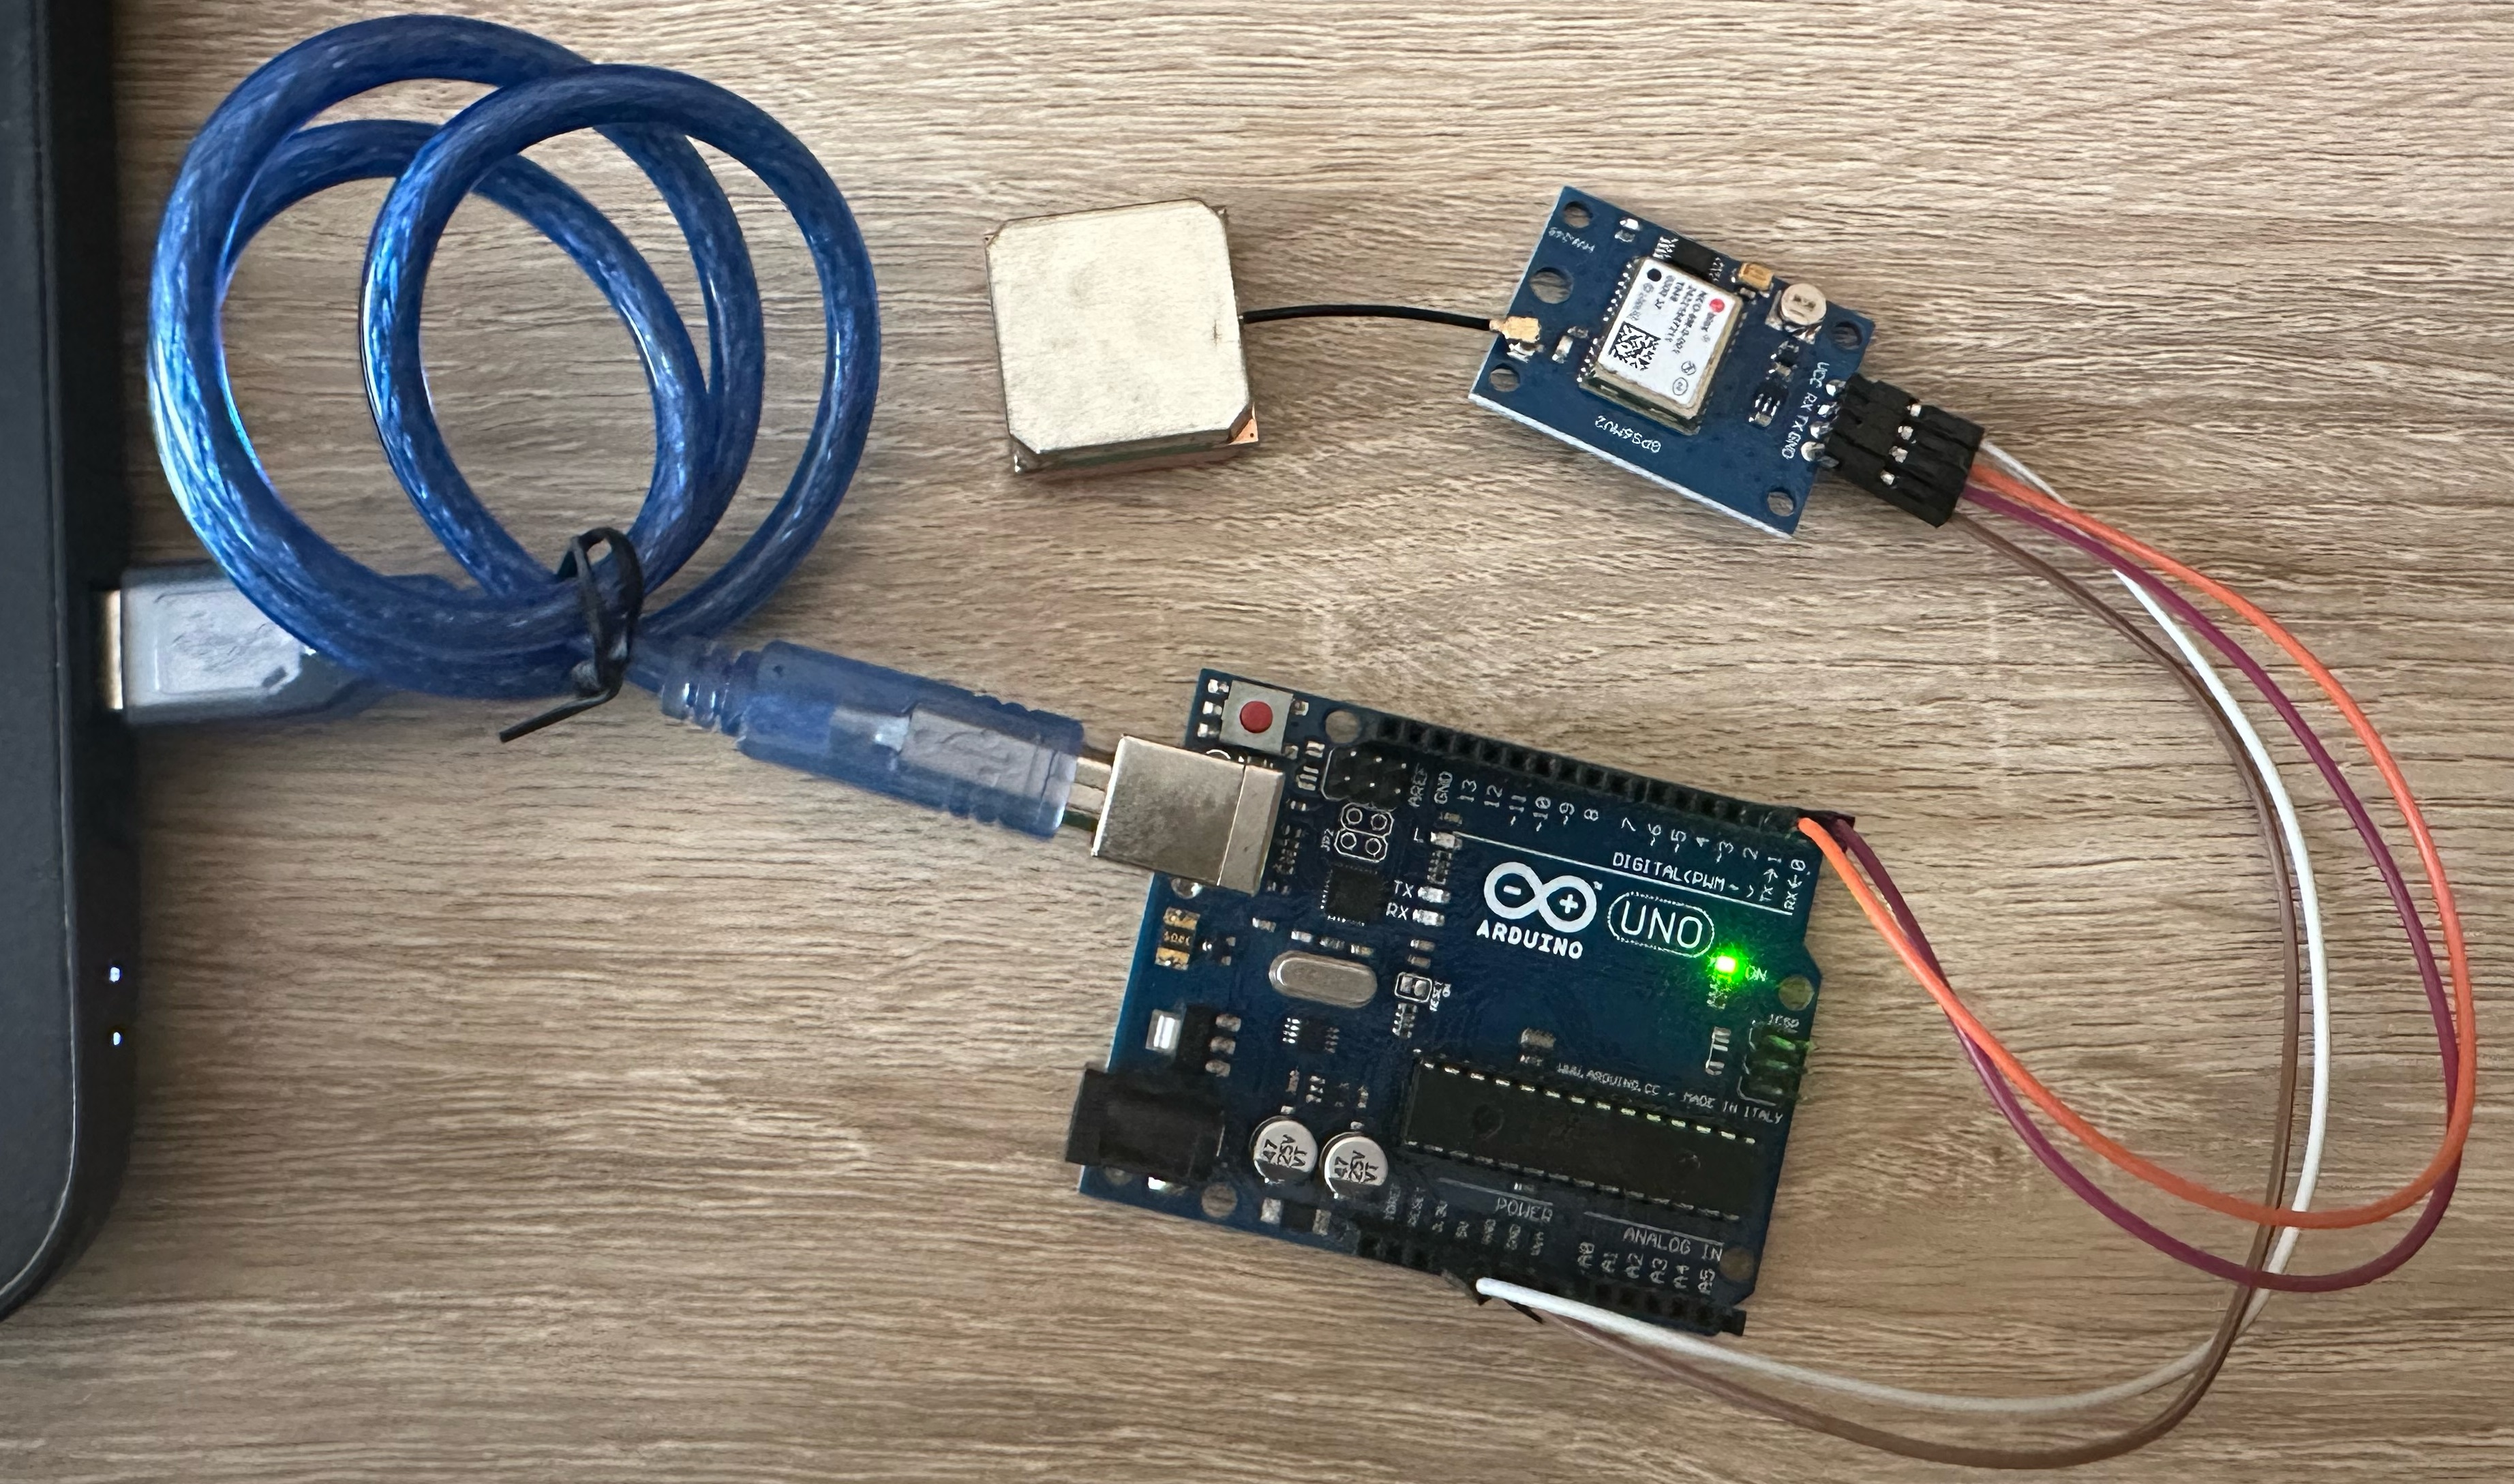
\includegraphics[width=0.45\textwidth, height=5cm]{imagenes/prueba-gps-uno.jpeg}}
    \quad
    \subfigure[) Usando el Arduino Pro Micro.]{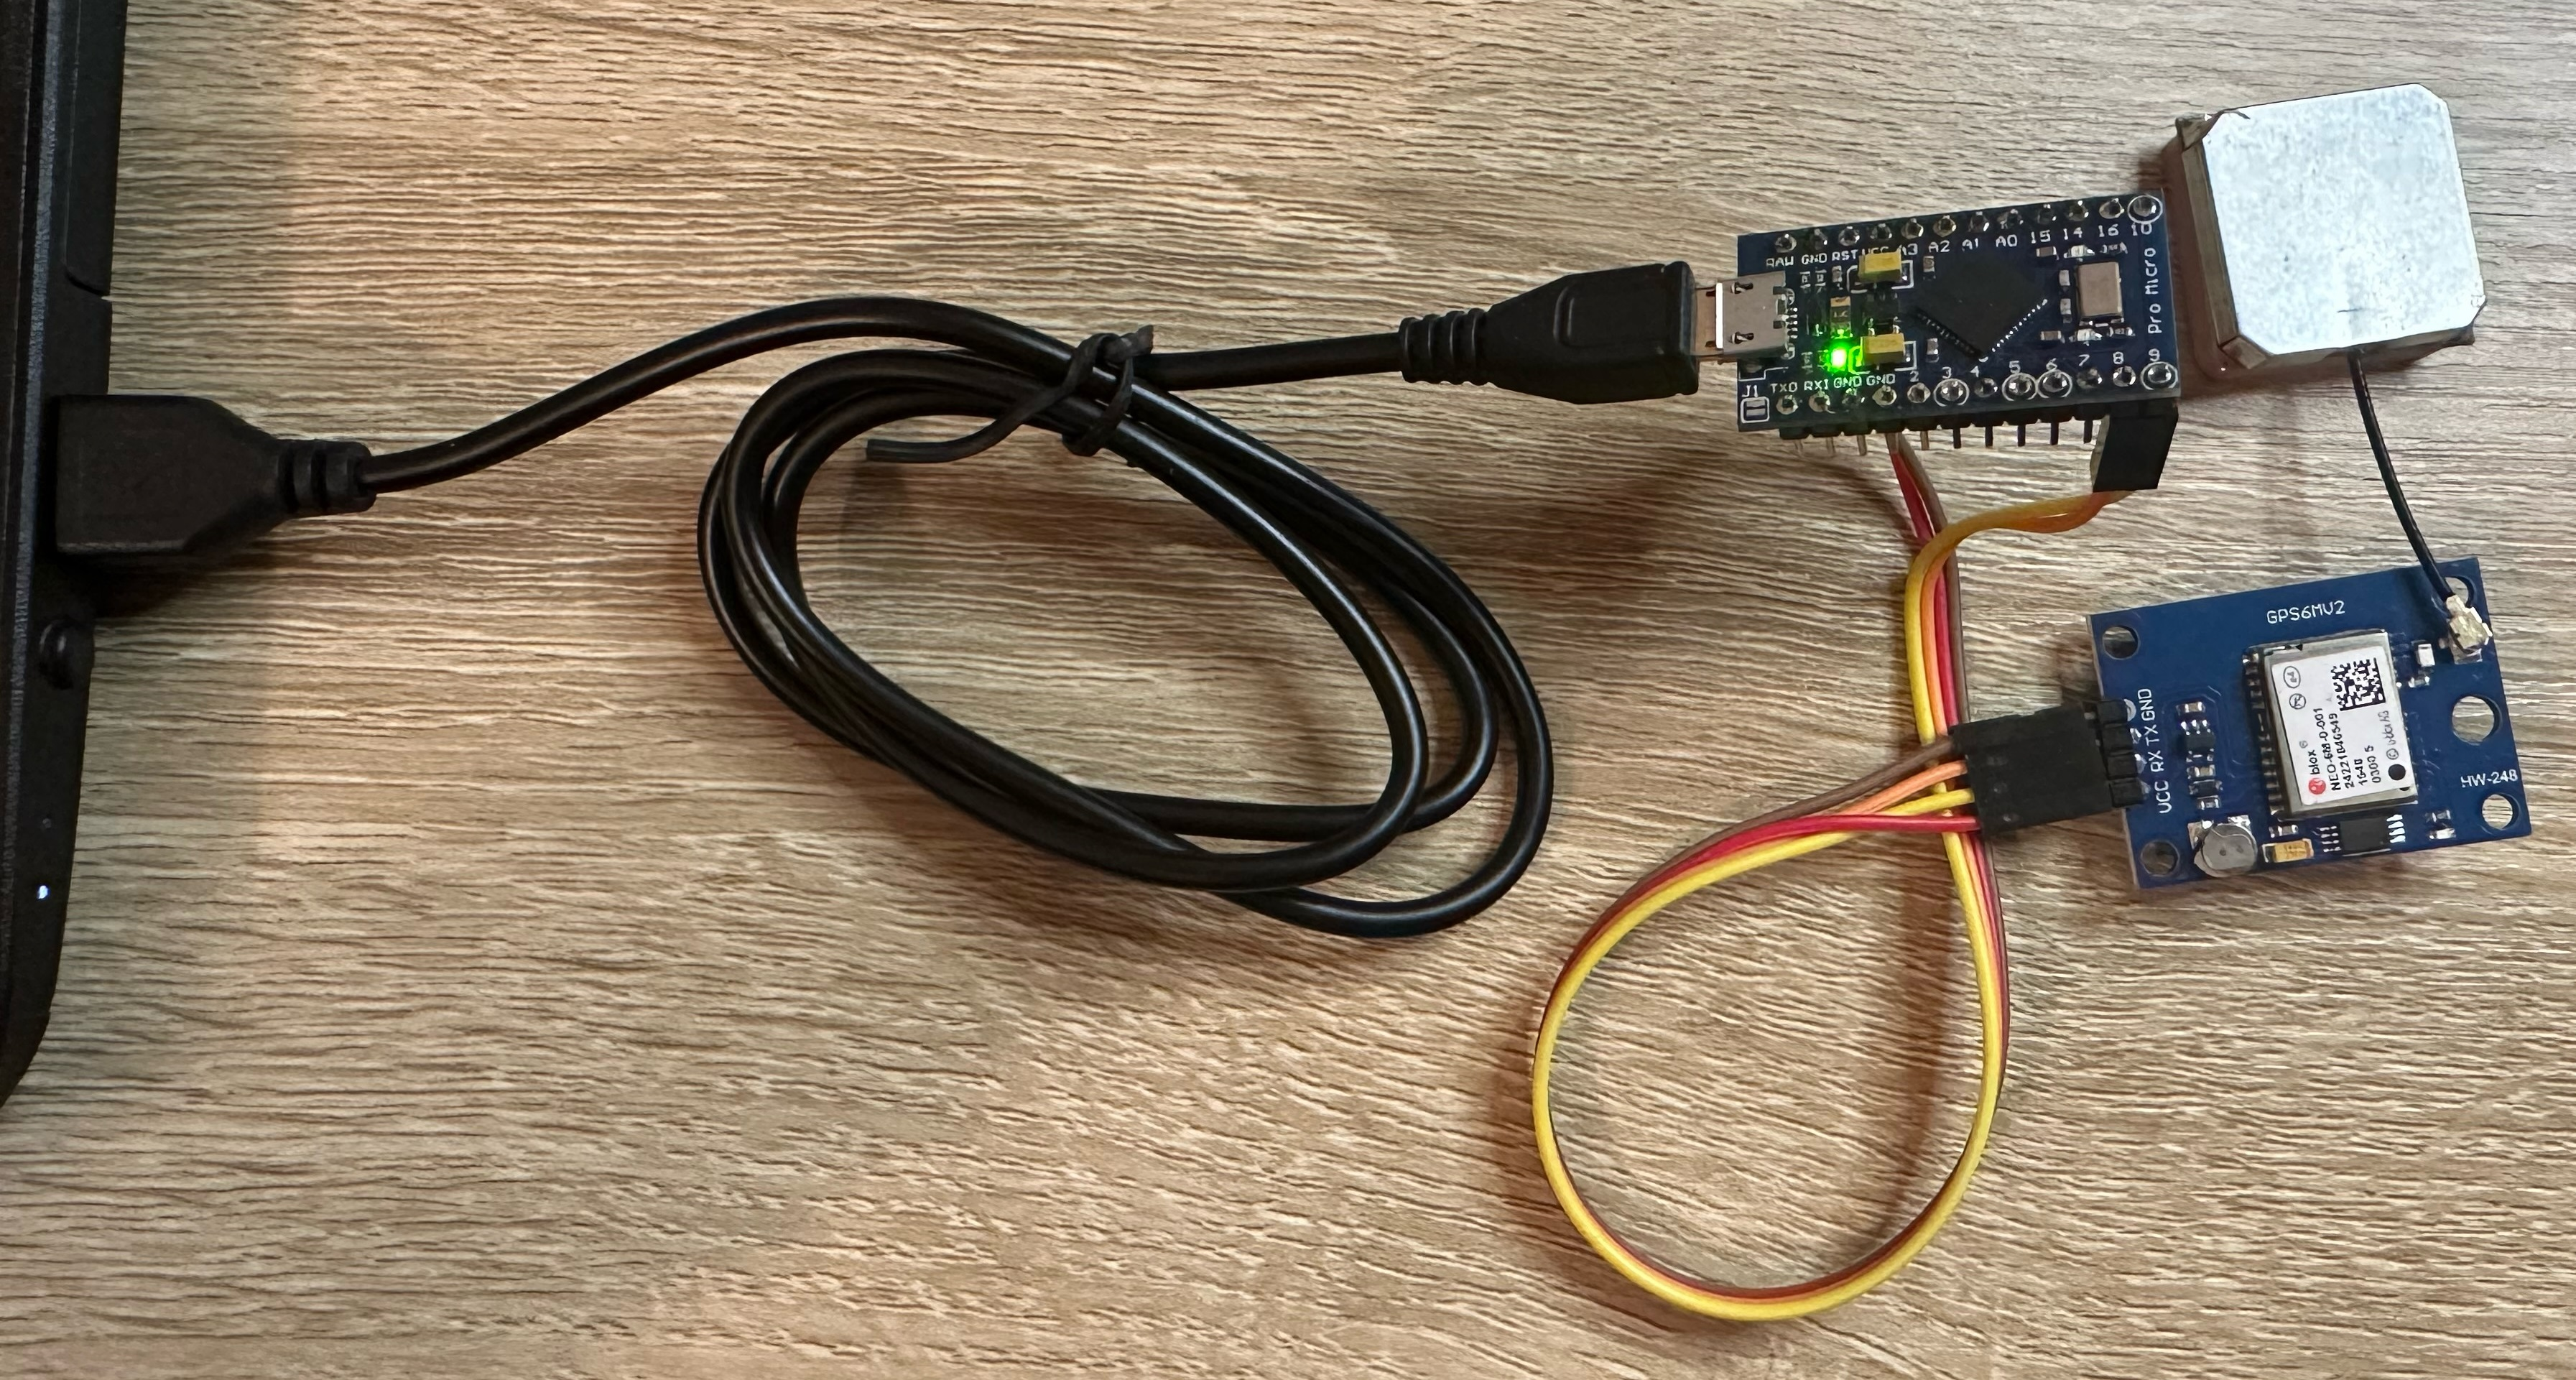
\includegraphics[width=0.45\textwidth, height=5cm]{imagenes/prueba-gps-micro.jpeg}}
    \caption{Prueba del GPS-6M.}
    \label{fig:prueba_gps}
\end{figure}

\item \textbf{Cámara Trampa PR-700:}

La cámara trampa se alimenta con 4 baterías AA (aunque tiene espacio para 8 baterías AA, para utilizar las otras 4 baterías si se llegara a acabar la carga de las primeras 4) o mediante el cable tipo Micro USB que viene incluido, utilizando una fuente de energía adecuada según las especificaciones del fabricante. Asegurándose de que la alimentación sea estable y suficiente para el funcionamiento óptimo de la cámara trampa durante el período de monitoreo.

Se ajustan los parámetros de la cámara trampa, como la resolución de imagen y la frecuencia de disparo, de acuerdo con los requisitos del proyecto, esto mediante el menú de configuración de la cámara trampa.

Después de la configuración, se procede a verificar que la cámara trampa pueda capturar imágenes de alta calidad y almacenarlas en una tarjeta de memoria de tipo MicroSD. Se coloca la cámara trampa en el lugar deseado y se activa para que comience a capturar imágenes. Se revisan las imágenes capturadas para evaluar su calidad y claridad. Se verifica que las imágenes sean nítidas y que capturen adecuadamente archivos multimedia cuando ocurre un movimiento en la zona durante el tiempo preestablecido.

\begin{figure}[H]
    \centering
    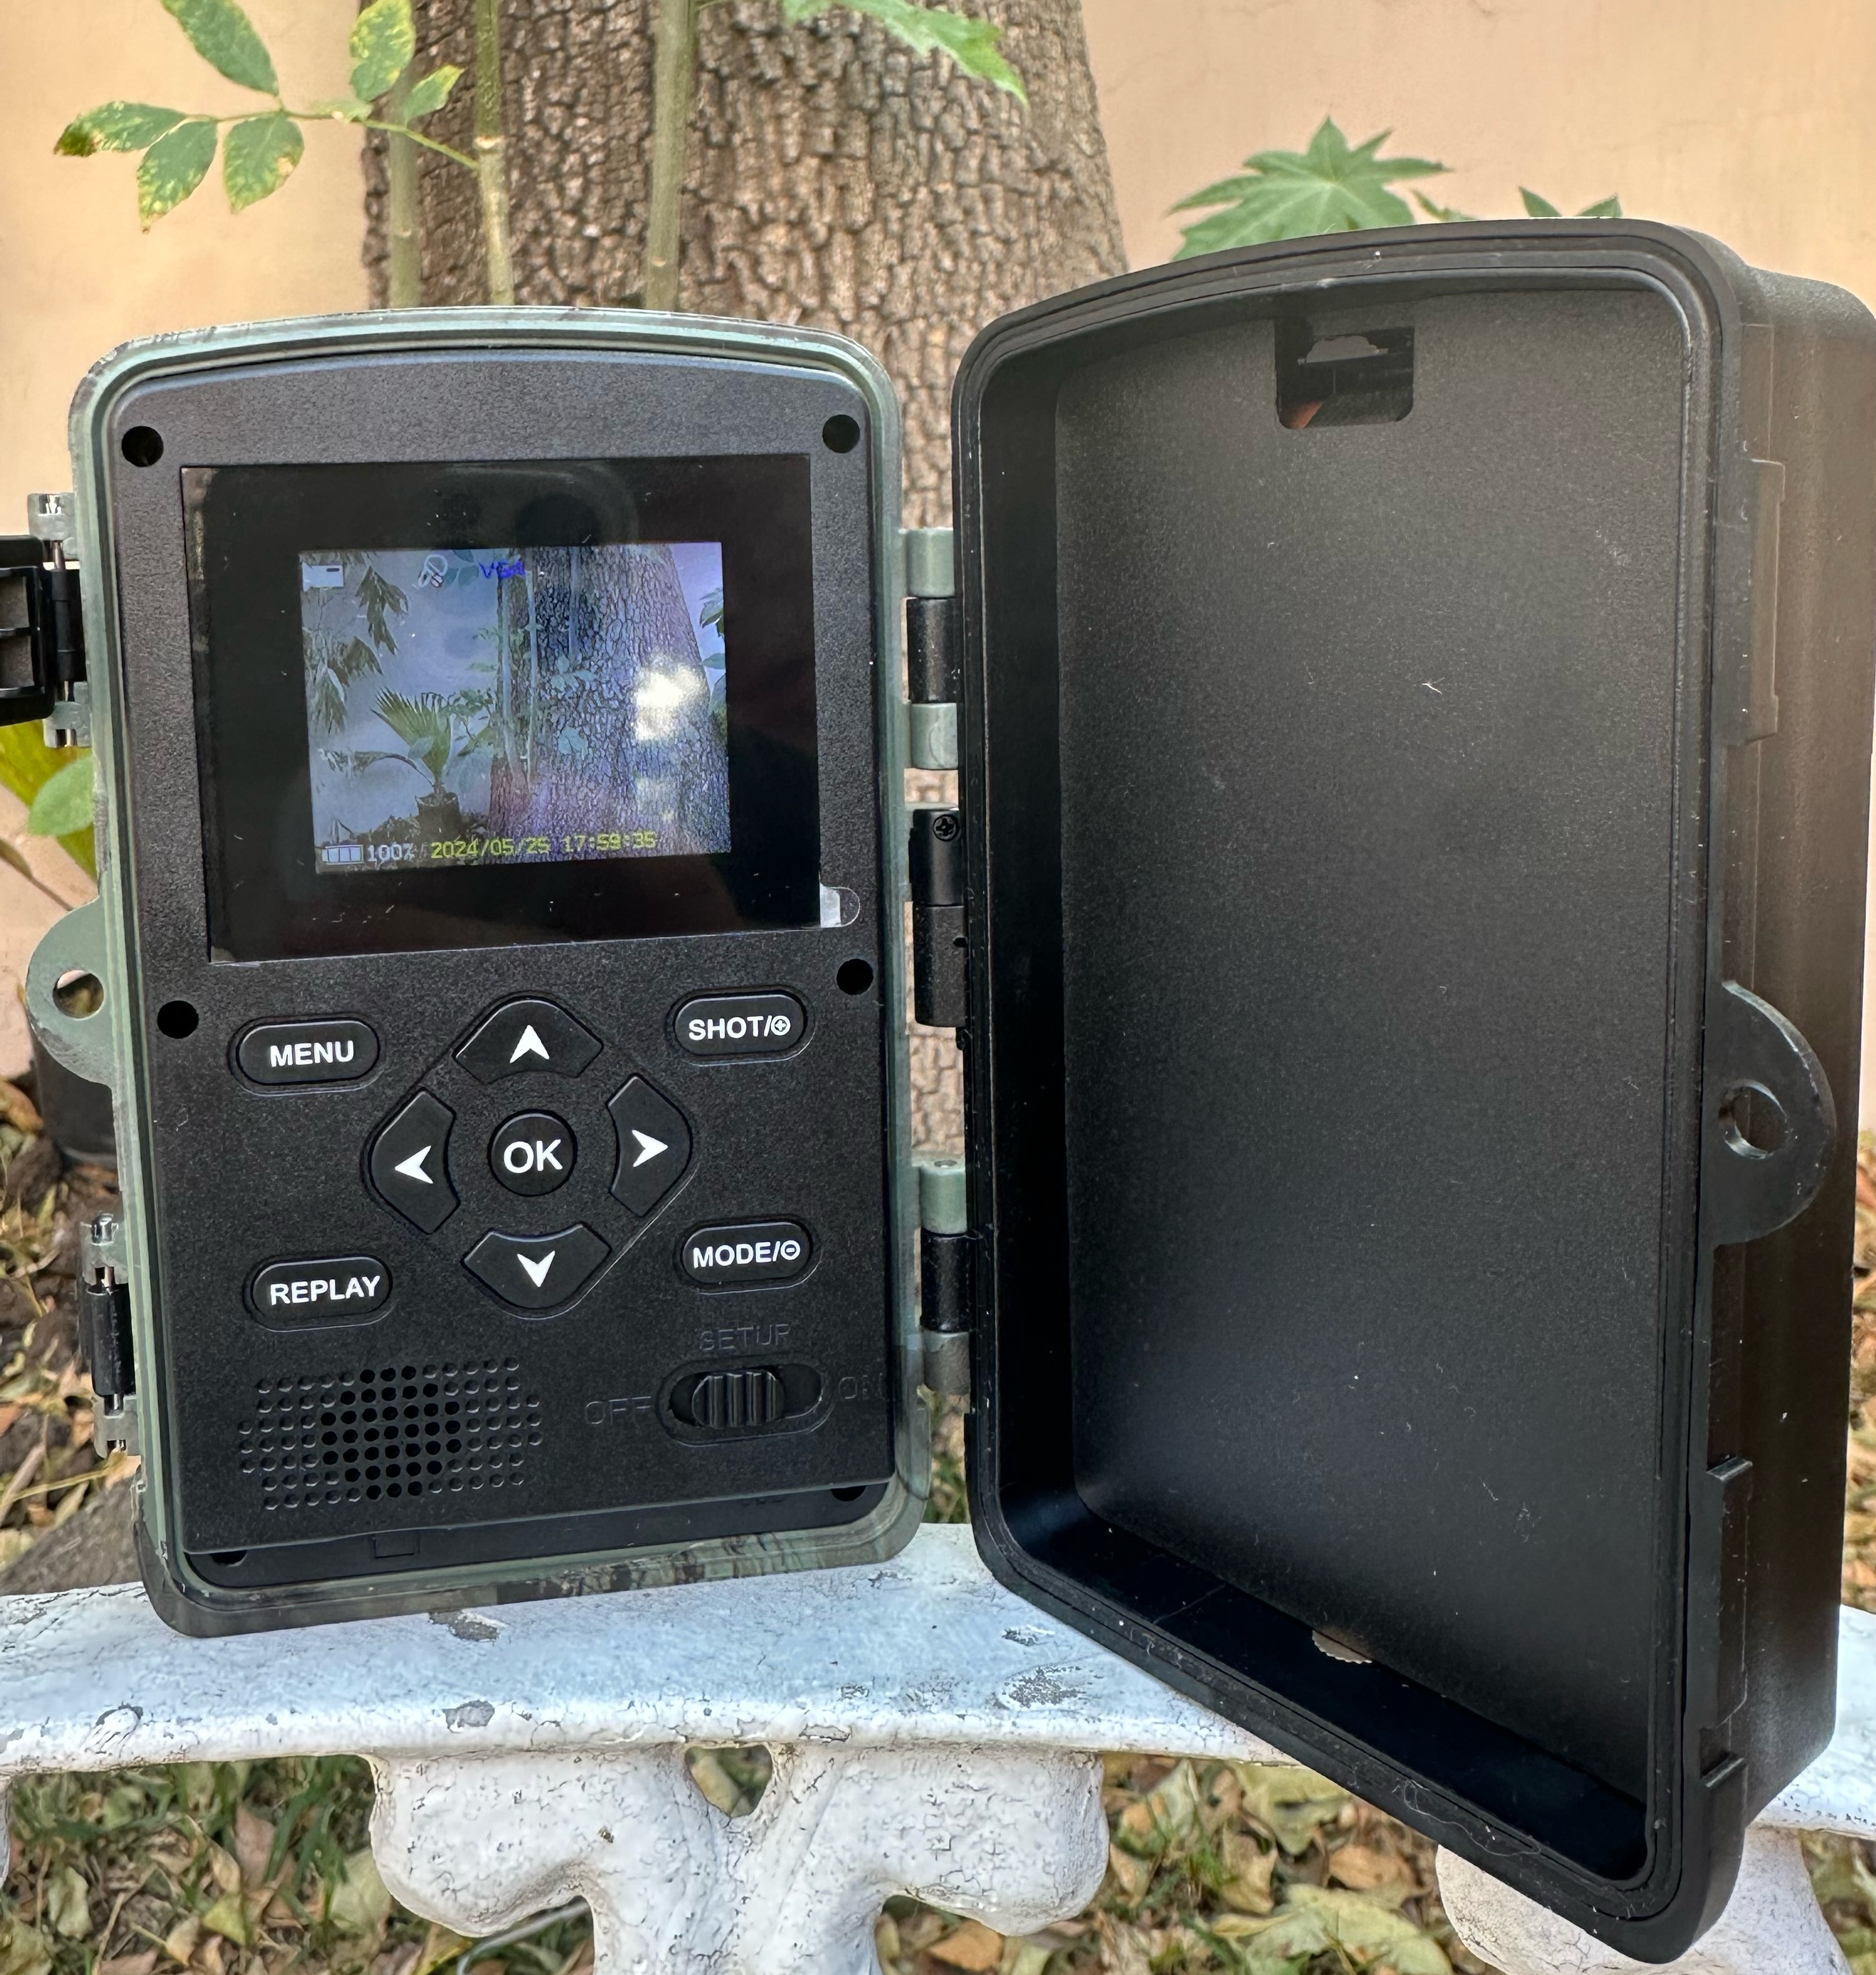
\includegraphics[height=7cm]{imagenes/prueba-camara.jpeg}
    \caption{Prueba de la cámara trampa PR-700.}
    \label{fig:prueba_camara_trampa}
\end{figure}


\item \textbf{Módulo LoRa UART 868/915 MHz:}

Se conecta el módulo LoRa a la placa Arduino siguiendo las especificaciones del fabricante. Es crucial asegurar una conexión adecuada para garantizar la comunicación efectiva entre los dispositivos.

Se configura el módulo LoRa para establecer la comunicación con otro módulo LoRa. Esto implica ajustar parámetros como la frecuencia de operación, el factor de propagación y la potencia de transmisión para garantizar una transmisión confiable de datos, utilizando la librería"LoRa\_E22.h", que proporcionan las funciones y definiciones necesarias para la comunicación y el control del módulo LoRa E22. También se configuran los pines utilizados para conectar el Arduino Pro Micro con el módulo LoRa E22, esto incluye los pines de recepción (Rx), transmisión (Tx), AUX (para indicaciones), y los pines M0 y M1 para configurar los modos de funcionamiento del módulo LoRa.

Se realizan pruebas de comunicación entre los módulos LoRa para confirmar la conectividad y la transmisión de datos sin errores. Enviando mensajes desde un módulo LoRa utilizando  la función `sendMessage()' y verificando que sean recibidos correctamente por el otro módulo con  la función `receiveMessage()'. Se realizan múltiples pruebas en diferentes condiciones para garantizar la robustez del sistema de comunicación.

\begin{figure}[H]
	\centering
	\subfigure[Transmisor.]{
		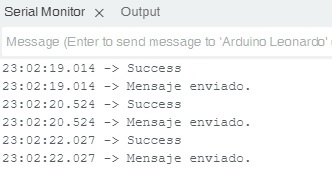
\includegraphics[width=0.37\textwidth, height=4cm]{imagenes/loratx_solo.jpg}
		\label{fig:transmisor}
	}
	\hspace{0.5cm} % Espacio vertical entre las imágenes
	\subfigure[Receptor.]{
		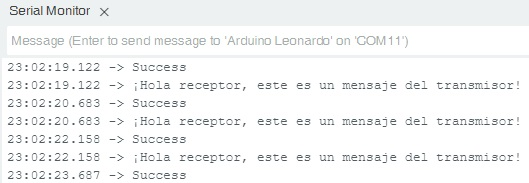
\includegraphics[width=0.37\textwidth, height=4cm]{imagenes/lorarx_solo.jpg}
		\label{fig:receptor}
	}
	\caption{Resultado de transmitir y recibir mediante los transceptores LoRa.}
	\label{fig:lora-solo}
\end{figure}





\begin{figure}[H]
    \centering
    \subfigure[) Transmisor.]{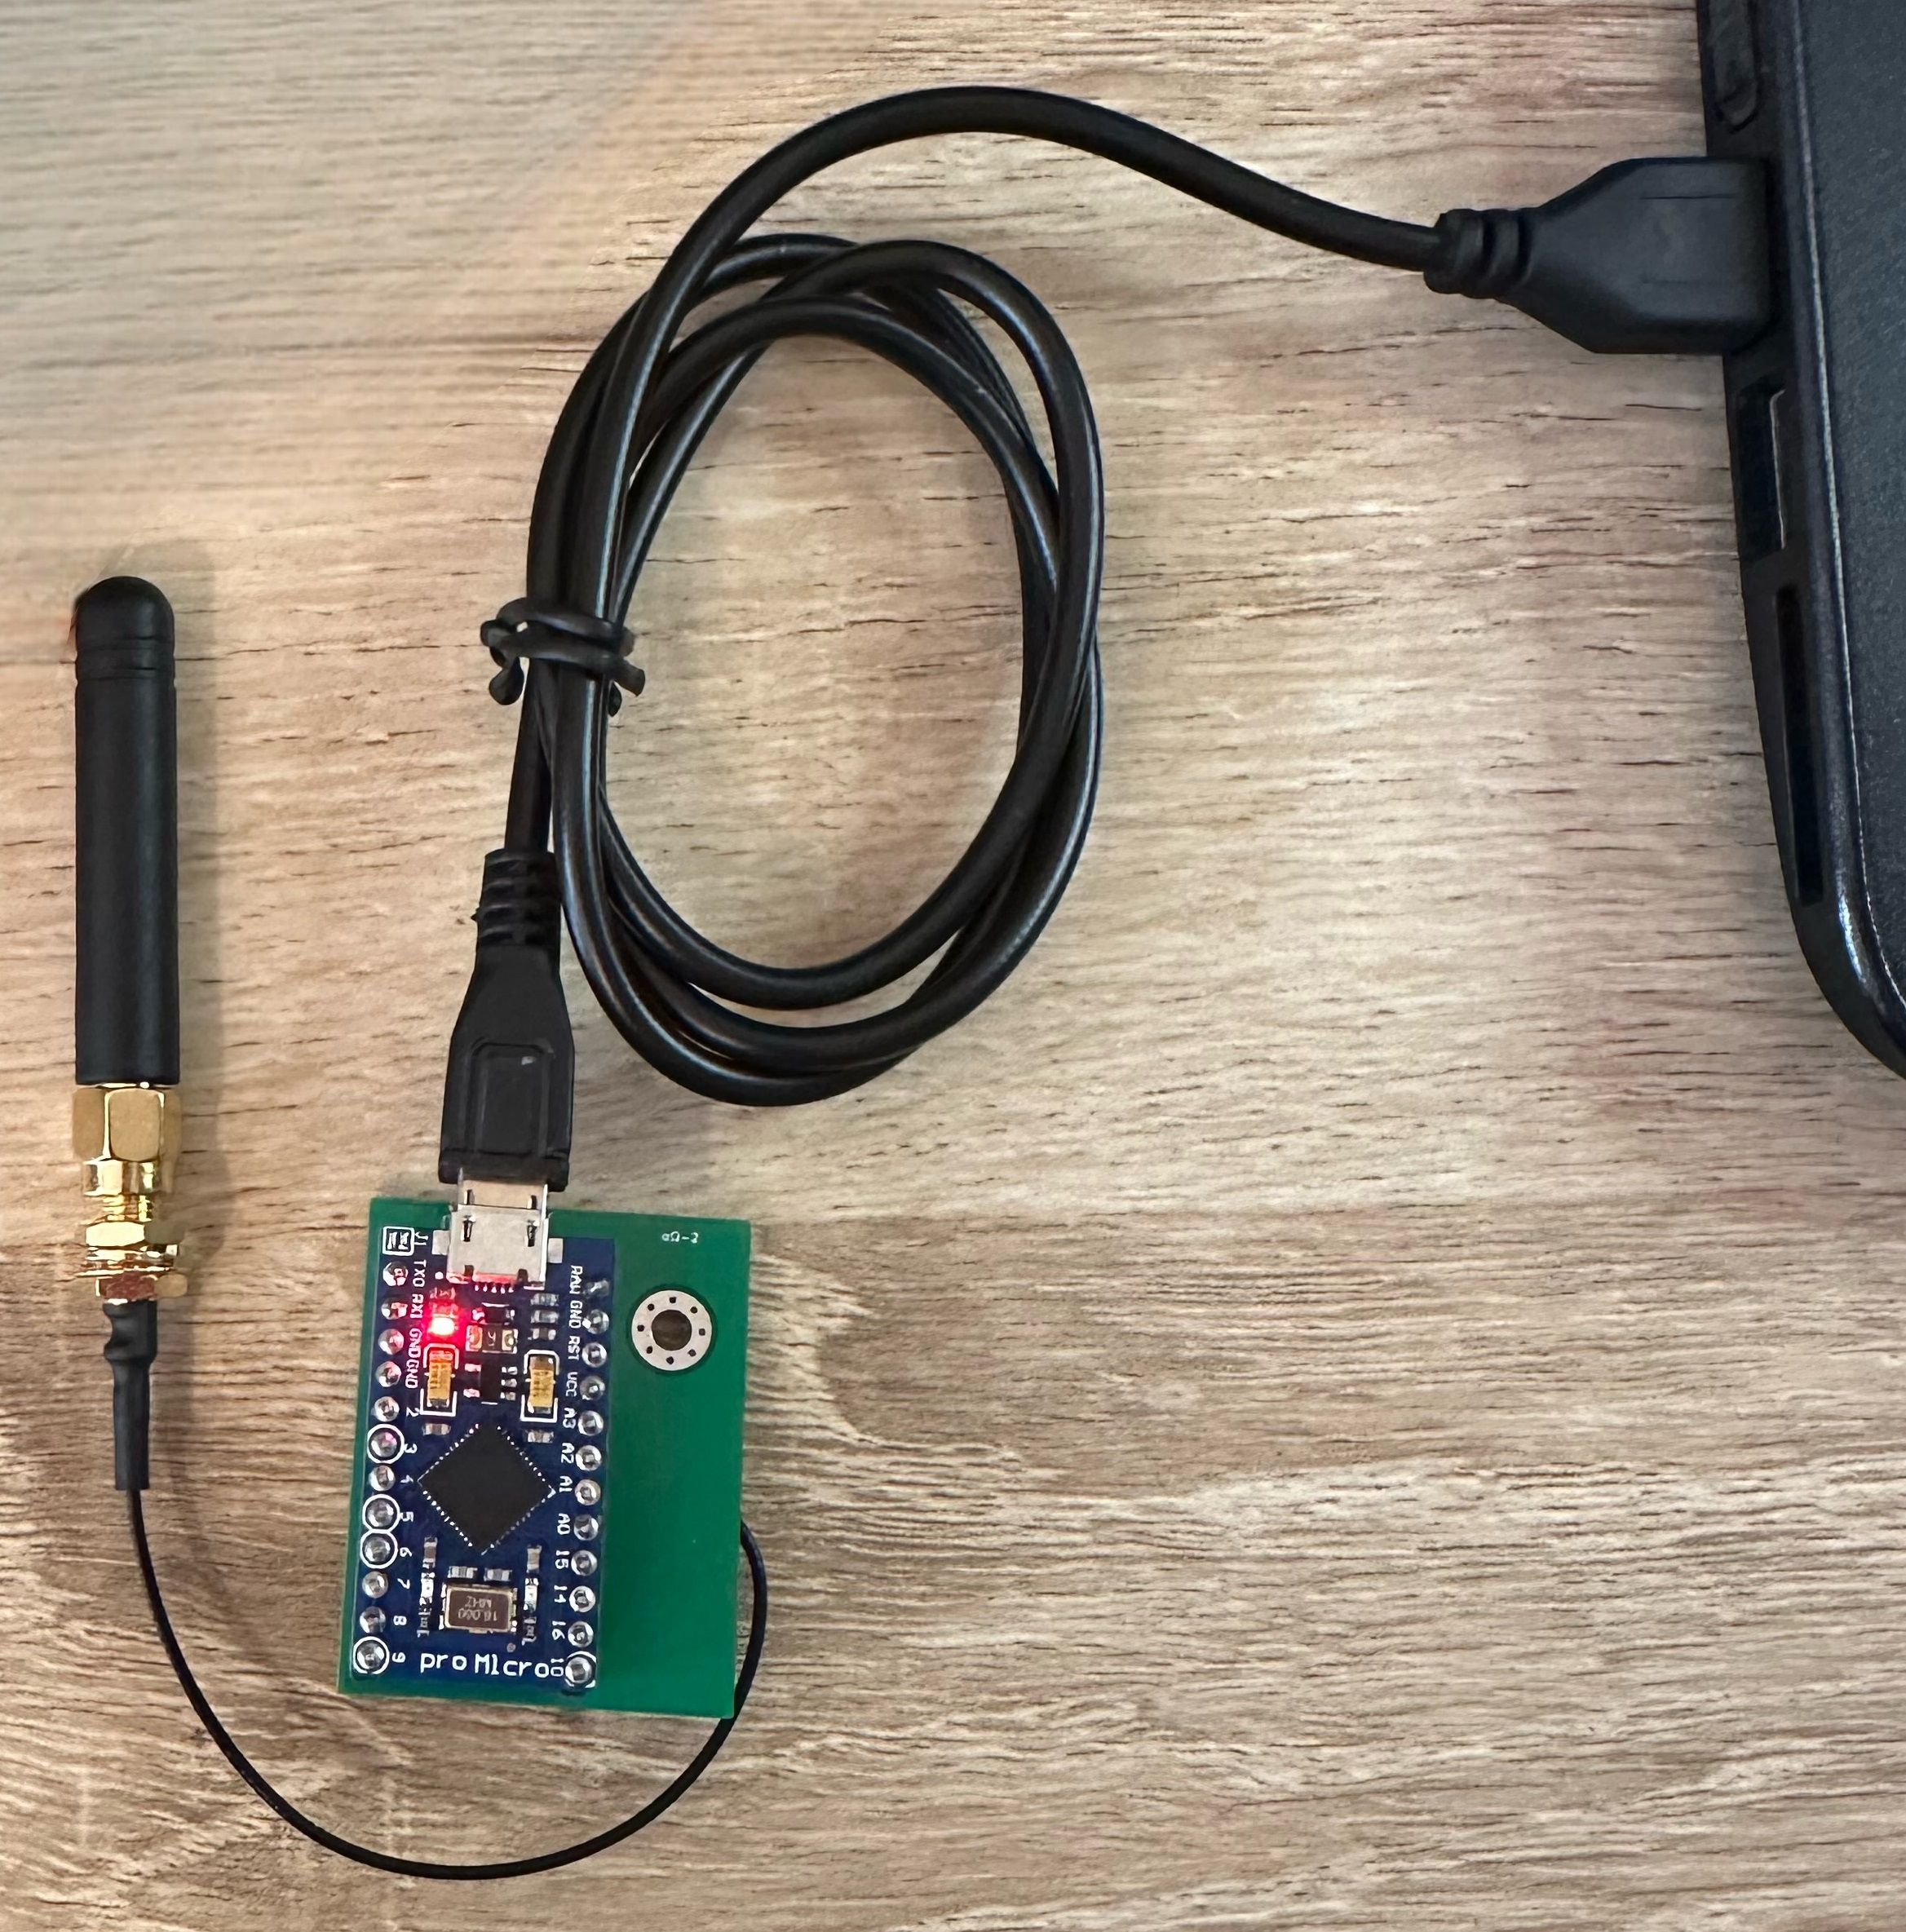
\includegraphics[width=0.45\textwidth, height=5cm]{imagenes/prueba-lora-tx.jpeg}}
    \quad
    \subfigure[) Receptor.]{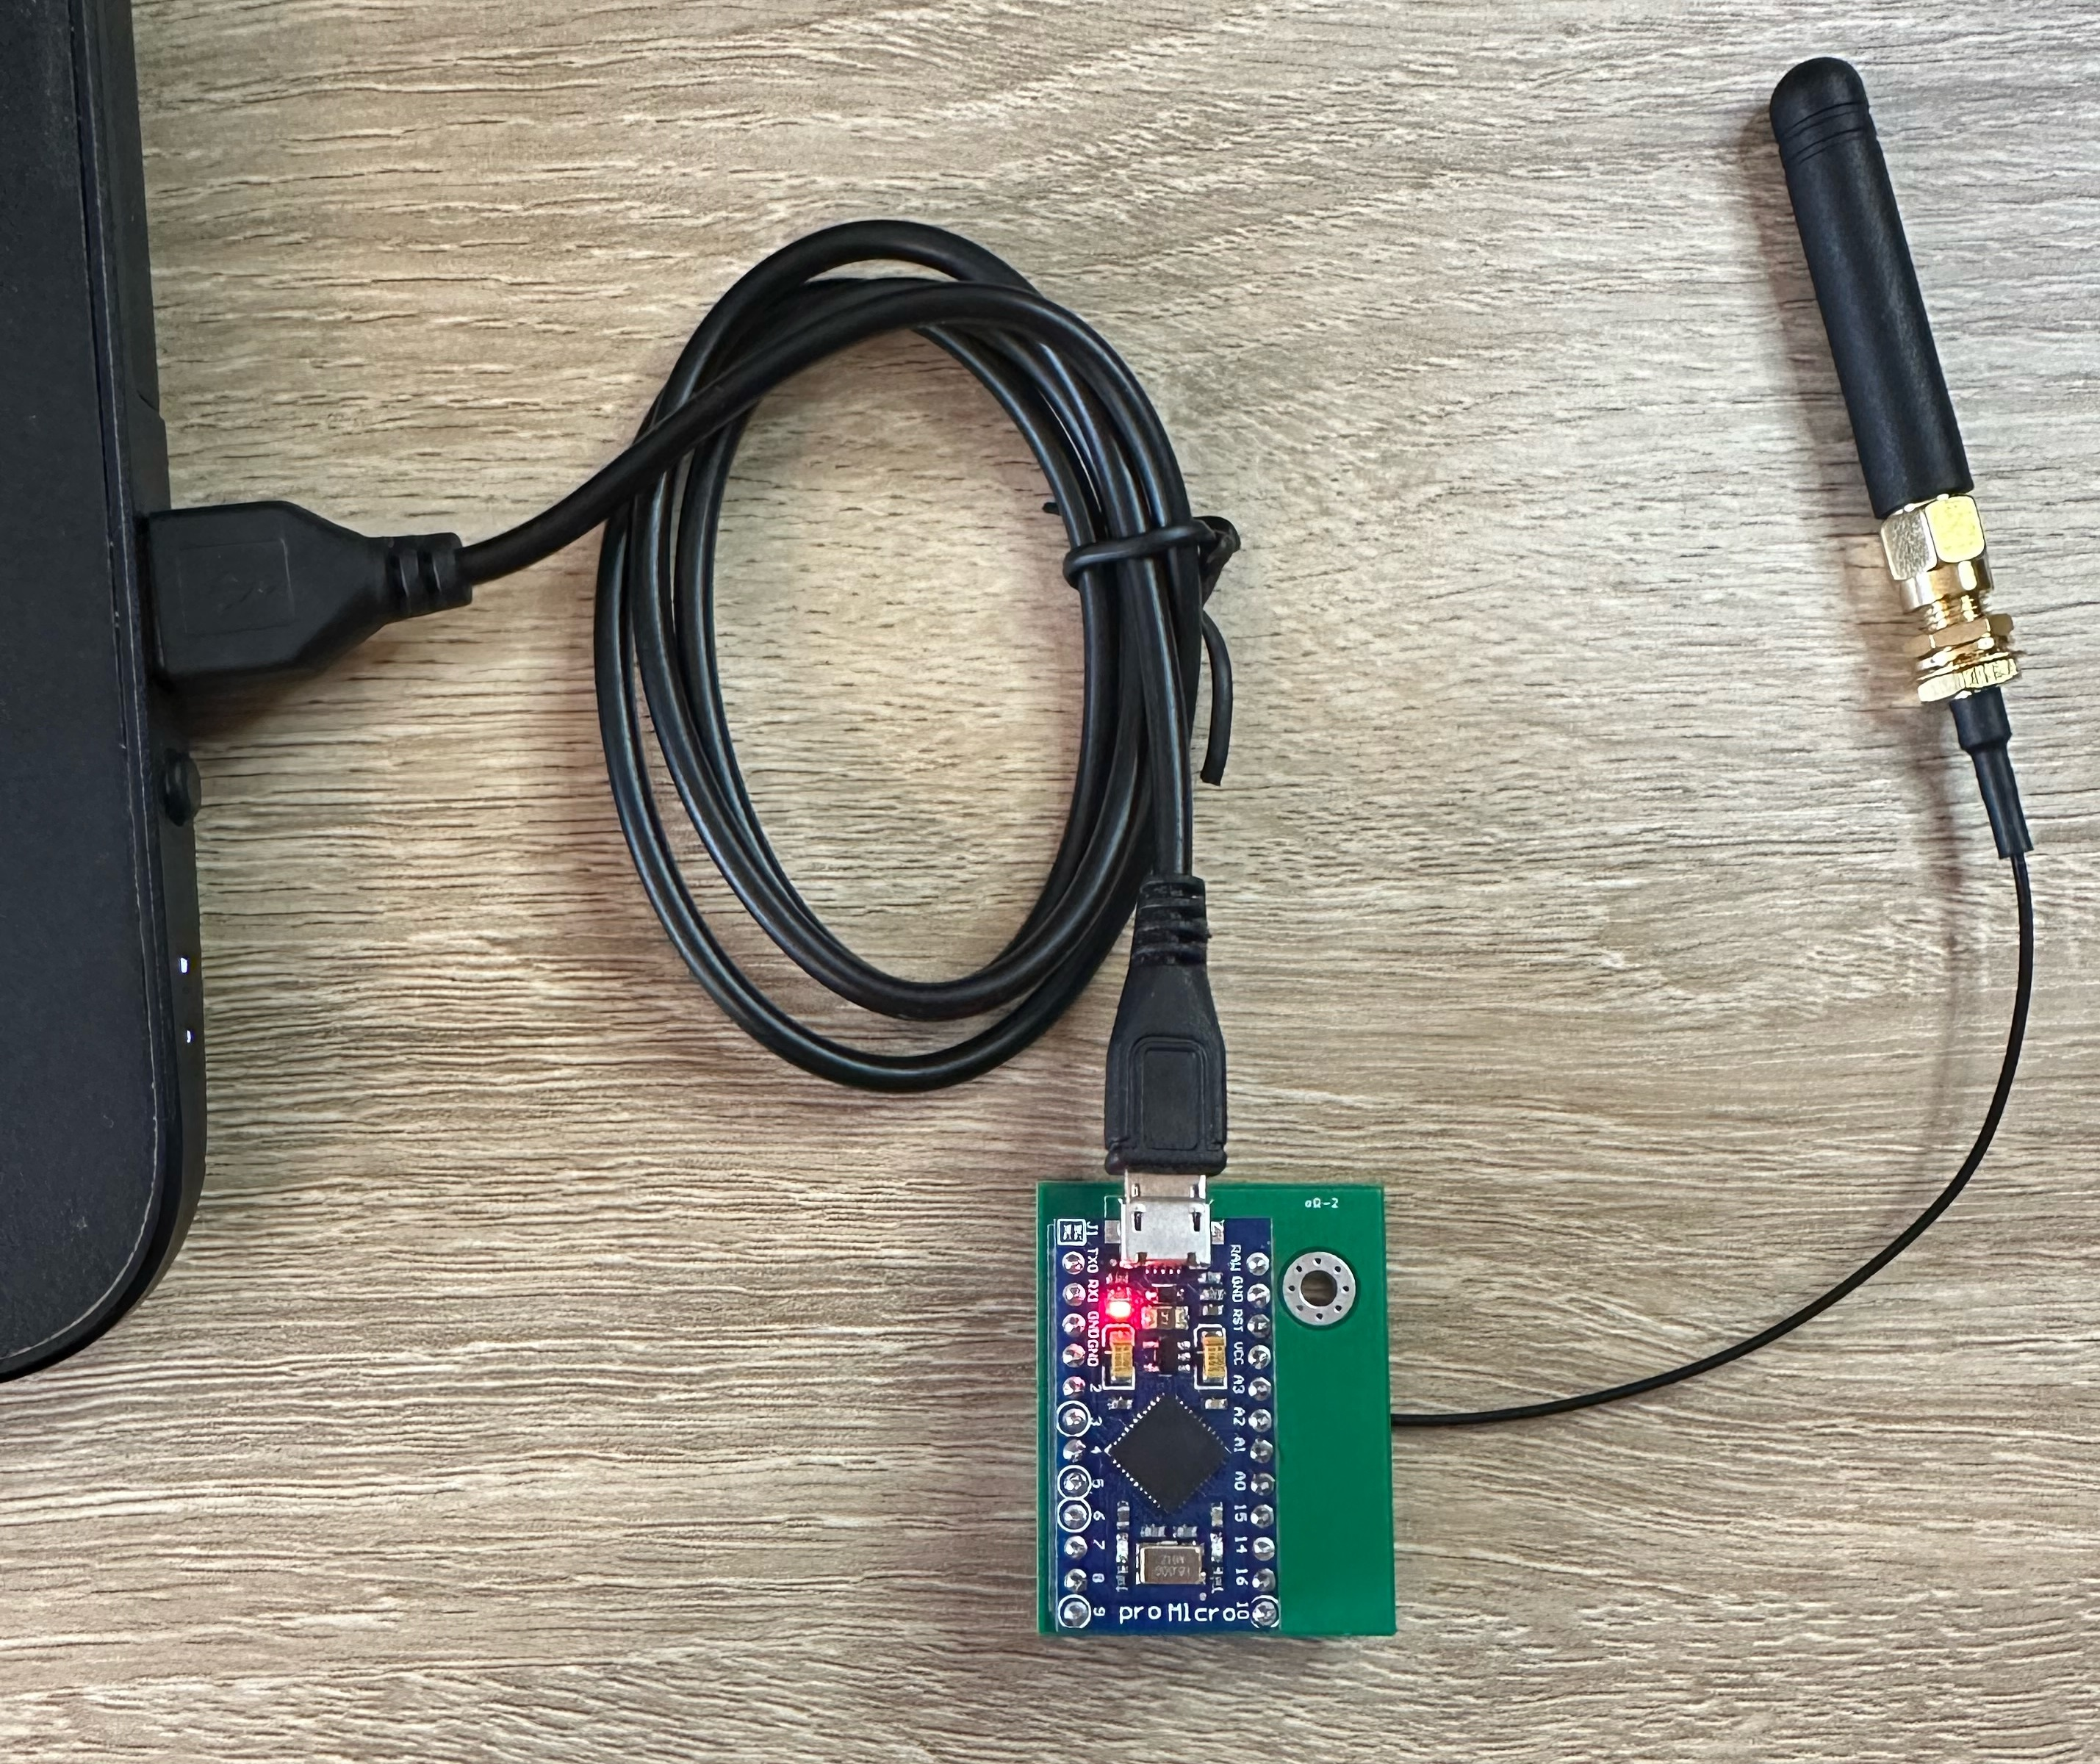
\includegraphics[width=0.45\textwidth, height=5cm]{imagenes/prueba-lora-rx.jpeg}}
    \caption{Prueba de los módulos LoRa usando Arduinos Pro Micro.}
    \label{fig:prueba_modulos_LoRa}
\end{figure}


\item \textbf{Módulo Adaptador MicroSD y Memorias MicroSD:}

Se inserta una tarjeta MicroSD en el módulo adaptador y se conecta este último a la placa de Arduino Pro Micro. Es importante asegurarse de que la tarjeta esté correctamente insertada. 

Después, se conecta físicamente el módulo adaptador MicroSD a la placa Arduino, siguiendo las siguientes conexiones de acuerdo a la librería utilizada llamada SD: el pin SCK se conecta al pin 15 de la placa (SCK del adaptador), MOSI al pin 16 (MOSI del adaptador), MISO al pin 14 (MISO del adaptador) y el ChipSelect del adaptador a un pin de elección de la placa Arduino Pro Micro(en nuestro caso se configuró el pin 10).

Posteriormente, se realizan pruebas de escritura y lectura de datos desde la tarjeta MicroSD para asegurarse de que la comunicación y el almacenamiento funcionen correctamente. Esto, implementa un menú interactivo en el monitor serial que permite al usuario seleccionar entre las opciones de escritura, lectura o borrado del archivo en la tarjeta MicroSD. Este menú proporciona una forma conveniente de probar las diferentes funciones que se pueden utilizar con la librería SD.

Una vez seleccionada una opción, se ejecuta el proceso correspondiente y se realizan las pruebas necesarias para verificar el correcto funcionamiento de cada función. Durante la escritura, se ingresan datos en el archivo en la tarjeta MicroSD. En el caso de la lectura, se recuperan los datos almacenados y se muestran en el monitor serial para su visualización. Para la opción de borrado, se elimina el archivo de la tarjeta MicroSD. El funcionamiento de este menú se puede observar en la Figura \ref{fig:memoria-solo}.

Después, se retira la tarjeta MicroSD y se coloca en otro dispositivo capaz de leer la tarjeta para así poder verificar la integridad de los datos almacenados. Se comparan estos datos leídos con los datos originales para asegurarse de que no haya errores de lectura o corrupción de datos.

\begin{figure}[H]
    \begin{minipage}{\textwidth}
        \centering
        \begin{minipage}{\textwidth}
            \centering
            \subfigure[) Escribir en el archivo.]{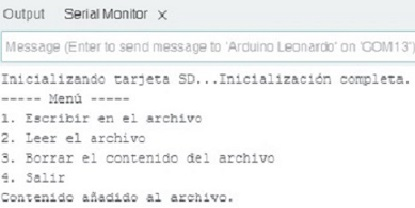
\includegraphics[width=0.45\textwidth, height=4cm]{imagenes/memoria_solo1.jpg}}
            \subfigure[) Leer el archivo.]{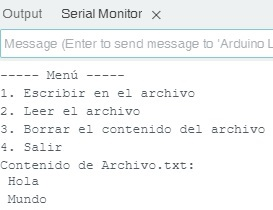
\includegraphics[width=0.45\textwidth, height=4cm]{imagenes/memoria_solo2.jpg}}
        \end{minipage}
    \end{minipage}
    \begin{minipage}{\textwidth}
        \centering
        \begin{minipage}{\textwidth}
            \centering
            \subfigure[) Borrar el archivo.]{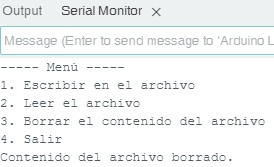
\includegraphics[width=0.45\textwidth, height=4cm]{imagenes/memoria_solo3.jpg}}
            \subfigure[) Salir del programa.]{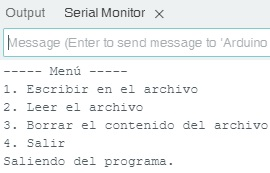
\includegraphics[width=0.45\textwidth, height=4cm]{imagenes/memoria_solo4.jpg}}
        \end{minipage}
\end{minipage}
\caption{Resultado de las funciones disponibles del adaptador MicroSD.}
\label{fig:memoria-solo}
\end{figure}

\begin{figure}[H]
    \centering
    \includegraphics[width=0.55\textwidth, height=4.6cm]{imagenes/prueba-adaptador.jpeg}
    \caption{Prueba del adaptador MicroSD usando el Arduino Pro Micro.}
    \label{fig:prueba_adaptador_MicroSD}
\end{figure}


\item \textbf{Baterías LiPo:}

Se utilizan cargadores compatibles para cargar completamente las baterías LiPo. Durante este proceso, se verifica que las baterías acepten la carga y que la tensión de salida sea la esperada mediante el uso de un multímetro.

Una vez que las baterías están completamente cargadas, se mide la tensión de salida para garantizar que esté dentro del rango especificado por el fabricante. Esta medida es crucial para asegurar un suministro de energía estable y confiable al sistema.

Después, se conectan las baterías LiPo al Arduino Pro Micro, asegurándose de que el positivo de la batería se conecte al pin RAW del Arduino y que la tierra se conecte al pin GND. Esta configuración garantiza un suministro de energía adecuado al Arduino y proporciona la conexión eléctrica necesaria para su funcionamiento dentro de la WSN.
\begin{figure}[H]
    \centering
    \includegraphics[width=0.55\textwidth, height=4cm]{imagenes/prueba-bateria.jpeg}
    \caption{Prueba de la batería LiPo para energizar el Arduino Pro Micro.}
    \label{fig:prueba_bateria_LiPo}
\end{figure}


\end{itemize}

Una vez completada la verificación de cada elemento individual, se procederá a la integración de los componentes en la red de sensores inalámbricos. Por lo que es fundamental que cada componente funcione correctamente para garantizar la fiabilidad del sistema en su conjunto.

\subsection{Integración de los Elementos}
Después de haber verificado el funcionamiento de los componentes de manera individual se llevará a cabo su integración. Explorando cómo almacenar los datos de temperatura y GPS en una tarjeta MicroSD para su posterior análisis y cómo utilizar la tecnología LoRa para la transmisión eficiente de estos datos entre nodos de la red. A través de estos procesos de integración, se espera obtener una red de sensores completamente funcional y lista para su despliegue en el campo.
\begin{itemize}
    \item \textbf{Almacenamiento de datos de temperatura en la tarjeta MicroSD:} Se almacenan los datos recopilados por el sensor de temperatura en la tarjeta MicroSD, mediante la conversión de los valores analógicos obtenidos del termistor a grados Celsius y guardándolos junto con una marca de tiempo en un archivo de texto en la tarjeta MicroSD, además se muestran estos datos en el Monitor Serial.

El código realizado comienza inicializando la comunicación serial y configurando un pin para alimentar el termistor directamente, ya que el pin de VCC será utilizado para alimentar el módulo adaptador MicroSD, también se le configura el chip select y se conectan los demás pines como en se vio en el Funcionamiento de los Elementos. Después, se inicializa la tarjeta MicroSD y se borra el archivo de temperatura en caso de ya existir.

En el bucle principal, se lee el valor analógico del termistor, se convierte a temperatura en grados Celsius y se obtiene la marca de tiempo en formato HH:MM:SS iniciando desde el encendido del Arduino utilizando la función millis() de la librería TimeLib. Esta información se muestra en el Monitor Serial y se guarda en un archivo de texto en la tarjeta MicroSD en el siguiente formato: "temperatura; hora".

\begin{figure}[H]
    \centering
    \subfigure[) Monitor Serial.]{\includegraphics[width=0.45\textwidth, height=4cm]{imagenes/temperatura_memoria.jpg}}
    \quad
    \subfigure[) Archivo de texto.]{\includegraphics[height=3cm]{imagenes/temperatura_memoria-txt.jpg}}
    \caption{Resultados de guardar la temperatura en la memoria MicroSD.}
    \label{fig:temp-memoria-code}
\end{figure}

\begin{figure}[H]
    \centering
    \includegraphics[width=0.55\textwidth, height=5.1cm]{imagenes/temp-memoria.jpeg}
    \caption{Integración del termistor y el módulo adaptador MicroSD.}
    \label{fig:temp-memoria}
\end{figure}

\item \textbf{Almacenamiento de datos GPS en la tarjeta MicroSD:} Se registran las coordenadas GPS en un archivo de texto en la tarjeta MicroSD utilizando un Arduino y un módulo GPS. Las coordenadas se registran junto con la hora actual en formato HH:MM:SS ajustada para la Ciudad de México (GMT-6).

El código comienza inicializando la comunicación serial con el módulo GPS utilizando una comunicación de software serial a través de los pines RX y TX del Arduino. Luego, se configura la velocidad de comunicación del módulo GPS y se inicializa la tarjeta MicroSD.

En el bucle principal, se lee continuamente la información del módulo GPS. Cuando se recibe un mensaje que comienza con "\$GPRMC" (el mensaje de datos mínimos recomendados de GPS), se procesa para extraer la hora actual, la latitud y la longitud. Estos datos se convierten a formato decimal y se ajusta la hora al huso horario de la Ciudad de México (GMT-6).

Luego, se crea una cadena con los datos de coordenadas y hora en el formato "latitud, longitud ; hora". Esta cadena se imprime en el Monitor Serial y se guarda en el archivo de texto en la tarjeta MicroSD.

\begin{figure}[H]
    \centering
    \subfigure[) Monitor Serial.]{\includegraphics[width=0.45\textwidth, height=4cm]{imagenes/gps_memoria.jpg}}
    \quad
    \subfigure[) Archivo de texto.]{\includegraphics[width=0.45\textwidth, height=4cm]{imagenes/gps_memoria-txt.jpg}}
    \caption{Resultados de guardar las coordenadas GPS en la memoria MicroSD.}
    \label{fig:temp-memoria-code}
\end{figure}

\begin{figure}[H]
    \centering
    \includegraphics[width=0.55\textwidth, height=5cm]{imagenes/gps-memoria.jpeg}
    \caption{Integración del GPS y el módulo adaptador MicroSD.}
    \label{fig:gps-memoria}
\end{figure}

\item \textbf{Transmisión de archivos desde la tarjeta MicroSD mediante LoRa:}
Este proyecto realiza un intercambio de archivos de texto entre dispositivos usando un Arduino Pro Micro, un módulo adaptador MicroSD y un módulo LoRa E22. El archivo de texto recibido se almacena en una tarjeta MicroSD y el usuario puede interactuar con el sistema mediante un menú en el monitor serial.

El menú permite al usuario seleccionar entre diferentes opciones: escribir en el archivo, leer el archivo, borrar el contenido del archivo y enviar el archivo por LoRa. Dependiendo de la opción seleccionada, se ejecuta la función correspondiente.

Durante la ejecución, el programa verifica continuamente si hay datos disponibles en el módulo LoRa. Si hay datos disponibles, estos se reciben y se almacenan en una variable. Los datos recibidos se muestran en el Monitor Serial para que el usuario pueda ver lo que se ha recibido y se guardan en un archivo txt en la tarjeta MicroSD. Si ocurre un error al intentar abrir el archivo, se notifica al usuario.

Por otra parte, para enviar el contenido del archivo, primeramente, se abre el archivo, después se guardan los datos en una variable y se envían a través del módulo LoRa. De igual forma , se notifica al usuario sobre el éxito o el fracaso del envío.

\begin{figure}[H]
    \begin{minipage}{\textwidth}
        \centering
        \begin{minipage}{\textwidth}
            \centering
            \subfigure[) Escribir en el archivo.]{\includegraphics[width=0.45\textwidth, height=4.5cm]{imagenes/lora_memoria1.jpg}}
            \subfigure[) Transmitir el archivo.]{\includegraphics[width=0.45\textwidth, height=4.5cm]{imagenes/lora_memoria2.jpg}}
        \end{minipage}
    \end{minipage}
\end{figure}
\newpage
\begin{figure}[H]
    \begin{minipage}{\textwidth}
        \centering
        \begin{minipage}{\textwidth}
            \centering
            \subfigure[) Leer el archivo.]{\includegraphics[width=0.45\textwidth, height=4.5cm]{imagenes/lora_memoria3.jpg}}
            \subfigure[) Archivo de texto recibido.]{\includegraphics[width=0.45\textwidth, height=3cm]{imagenes/lora_memoria4.jpg}}
        \end{minipage}
    \end{minipage}
    \caption{Resultados de transmitir el archivo txt de la memoria MicroSD usando LoRa.}
    \label{fig:lora-memoria}
\end{figure}

\begin{figure}[H]
    \centering
    \subfigure[) Transmisor.]{\includegraphics[width=0.45\textwidth, height=5cm]{imagenes/lora-tx-memoria.jpeg}}
    \quad
    \subfigure[) Receptor.]{\includegraphics[width=0.45\textwidth, height=5cm]{imagenes/lora-rx-memoria.jpeg}}
    \caption{Integración del módulo adaptador MicroSD y el transceptor LoRa.}
    \label{fig:lora-memoria-img}
\end{figure}

\item \textbf{Almacenamiento de datos GPS en la tarjeta MicroSD con transmisión mediante LoRa:} 
Este proyecto permite registrar coordenadas GPS en una tarjeta MicroSD y transmitir estos datos a través de una transceptores LoRa. Utiliza un Arduino, un módulo GPS, un módulo adaptador MicroSD, un módulo LoRa E22 y una tarjeta MicroSD para realizar estas tareas.

El sistema comienza con la inicialización de la tarjeta MicroSD. Si la tarjeta no se inicializa correctamente, se notifica al usuario y el programa se detiene. A continuación, se configura el módulo GPS para comunicarse a través de una conexión serial, ajustando la velocidad de comunicación del módulo GPS NEO-6M. Posteriormente, se inicializa el módulo LoRa E22, preparándolo para la transmisión de datos.

El módulo GPS se utiliza para recibir datos de ubicación en formato NMEA, que incluye información sobre la latitud, longitud y hora. Estos datos se procesan para extraer las coordenadas y la hora actual, convirtiendo las coordenadas a un formato decimal y ajustando la hora al huso horario de la Ciudad de México (GMT-6).

Las coordenadas GPS y la hora se guardan en un archivo de texto en la tarjeta MicroSD, actualizándose cada vez que se reciben nuevos datos GPS. El sistema abre el archivo en modo de escritura, guarda los datos y luego cierra el archivo para asegurar que la información se almacene correctamente.

Después, se define un intervalo de tiempo en el que se estarán guardando las coordenadas en la tarjeta y concluyendo este tiempo se iniciará la transmisión del archivo. Donde se lee el contenido del archivo y se envía a través del módulo LoRa. La transmisión se realiza en varios pasos: primero se envía un mensaje de inicio, seguido del nombre del archivo y luego cada línea de datos. Finalmente, se envía un mensaje de finalización para indicar que la transmisión ha terminado. Si la transmisión es exitosa, el archivo en la tarjeta MicroSD se borra para preparar el sistema para la próxima serie de datos.

Aunque el sistema opera principalmente de forma autónoma, la comunicación con el usuario se realiza a través del Monitor Serial. El usuario puede ver mensajes que indican el estado de la inicialización, la lectura de datos, el almacenamiento y la transmisión. Ilustrando así cómo integrar múltiples tecnologías (GPS, MicroSD y LoRa) para crear un sistema de registro y transmisión de datos eficiente, ideal para aplicaciones que requieren seguimiento de ubicación y comunicación inalámbrica.

\begin{figure}[H]
    \begin{minipage}{\textwidth}
        \centering
        \begin{minipage}{\textwidth}
            \centering
            \subfigure[) Transmisor.]{\includegraphics[width=0.45\textwidth, height=4.5cm]{imagenes/loratx_gps_memoria.jpg}}
            \subfigure[) Receptor.]{\includegraphics[width=0.45\textwidth, height=3.5cm]{imagenes/lorarx_gps_memoria.jpg}}
        \end{minipage}
    \end{minipage}
    \caption{Resultados de guardar las coordenadas en un archivo txt en la memoria MicroSD y trasmitirlo usando LoRa.}
\end{figure}

\begin{figure}[H]
    \centering
    \subfigure[) Transmisor.]{\includegraphics[width=0.45\textwidth, height=6.5cm]{imagenes/lora-gps-memoria.jpeg}}
    \quad
    \subfigure[) Receptor.]{\includegraphics[width=0.45\textwidth, height=6.5cm]{imagenes/lora-rx-memoria.jpeg}}
    \caption{Integración del GPS, el módulo adaptador MicroSD y el transceptor LoRa.}
    \label{fig:lora-memoria-img}
\end{figure}

\item \textbf{Recepción y almacenamiento de datos GPS mediante LoRa junto con datos de temperatura en la tarjeta MicroSD:} 
En este proyecto, se establece el sistema de recepción de datos GPS mediante LoRa, el cual almacena estos datos recibidos en una tarjeta MicroSD con el nombre de archivo recibido, a la par que almacena datos de temperatura. Utilizando un Arduino Pro Micro, un módulo GPS, un termistor, un módulo LoRa E22 y una tarjeta MicroSD.

Al iniciar, el sistema configura y alimenta el termistor, el módulo LoRa, y la tarjeta MicroSD. Si la inicialización del dispositivo de almacenamiento falla, se notifica al usuario y se detiene la ejecución para evitar errores posteriores. Una vez que todo está configurado correctamente, el sistema entra en el bucle principal donde se ejecutan dos tareas principales: la lectura y almacenamiento de la temperatura, y la recepción de archivos a través de LoRa.

La primera tarea es la lectura de la temperatura. El sistema lee el valor analógico del termistor, convierte este valor a grados Celsius, y obtiene la hora actual utilizando la librería TimeLib. La temperatura y la hora se imprimen en el Monitor Serial y se almacenan en un archivo en la tarjeta MicroSD. Este proceso se repite cada intervalo de tiempo establecido, proporcionando un registro continuo de la temperatura ambiental.

La segunda tarea es la recepción de archivos a través de LoRa. El sistema espera mensajes del módulo LoRa, y cuando recibe un mensaje de inicio (``START''), procede a recibir el nombre del archivo. Una vez recibido el nombre, se crea (en caso de no existir aún) y abre un archivo con ese nombre en la tarjeta MicroSD y se empiezan a recibir los datos del archivo. Los datos se almacenan línea por línea hasta que se recibe un mensaje de finalización (``END''). Si hay algún error en la recepción de los mensajes o al abrir el archivo, se notifica al transmisor para que no borre el archivo transmitido.

Combinando de esta forma, la recepción de datos GPS mediante LoRa con el almacenamiento de datos de temperatura en una tarjeta MicroSD. Utilizando tecnologías de comunicación inalámbrica y almacenamiento digital, se crea una solución robusta para la recopilación y registro de datos ambientales y de ubicación, adecuada para diversas aplicaciones en monitoreo remoto y seguimiento de activos.

\begin{figure}[H]
    \begin{minipage}{\textwidth}
        \centering
        \begin{minipage}{\textwidth}
            \centering
            \subfigure[) Monitor serial.]{\includegraphics[width=0.5\textwidth]{imagenes/lorarx_gps_temp_memoria.jpg}}
            \subfigure[) Archivos generados.]{\includegraphics[width=0.7\textwidth]{imagenes/archivos-lorarx_gps_temp_memoria.jpg}}
        \end{minipage}
    \end{minipage}
    \caption{Resultados de recibir las coordenadas usando LoRa, guardarlo en un archivo txt en la memoria MicroSD y recolectar datos de temperatura a la par.}
\end{figure}

\begin{figure}[H]
    \centering
    \subfigure[) Transmisor.]{\includegraphics[width=0.45\textwidth, height=6cm]{imagenes/lora-gps-memoria.jpeg}}
    \quad
    \subfigure[) Receptor.]{\includegraphics[width=0.45\textwidth, height=6cm]{imagenes/lora-rx-temp-memoria.jpeg}}
    \caption{Integración del GPS, el termistor, el módulo adaptador MicroSD y el transceptor LoRa.}
    \label{fig:lora-memoria-img}
\end{figure}

\item \textbf{Transmisión de datos GPS y de temperatura de la tarjeta MicroSD mediante LoRa:} 
En este proyecto, se establece un sistema para la transmisión de datos GPS y de temperatura contenidos en archivos de texto en una tarjeta MicroSD utilizando la tecnología LoRa. El sistema está compuesto por un Arduino Pro Micro, un termistor, un módulo LoRa E22, y una tarjeta MicroSD. La función principal es enviar los datos almacenados en la tarjeta MicroSD a través del módulo LoRa a un receptor remoto.

El programa comienza con la configuración inicial de los componentes. Se configuran los pines del módulo LoRa y de la tarjeta MicroSD. El módulo LoRa es configurado utilizando la biblioteca LoRa\_E22, y la tarjeta MicroSD es inicializada utilizando la biblioteca SD. Si la tarjeta no se inicializa correctamente, se notifica al usuario y el programa se detiene para evitar errores posteriores.

En el bucle principal, el sistema opera en tres modos principales de operación: recepción de archivos GPS por LoRa, medición y almacenamiento de temperatura, y transmisión de archivos GPS y de temperatura. Respecto a la recepción por LoRa, el Arduino monitorea continuamente la disponibilidad de mensajes mediante el módulo LoRa. Cuando se detecta un mensaje de inicio (``START''), se inicia la recepción del archivo correspondiente. Esto implica la espera y recepción del nombre del archivo a través de LoRa, seguido por la recepción secuencial de cada línea de datos. Cada línea de datos recibida se guarda directamente en un archivo con su correspondiente nombre en la tarjeta MicroSD, repitiendo esto hasta recibir un mensaje de finalización (``END''). Notificando al transmisor si ocurrió algún error en la recepción de los datos para anular la eliminación del archivo en el transmisor. 

Por otro lado, el Arduino también realiza mediciones periódicas de temperatura a intervalos regulares establecidos. Durante cada ciclo de medición, el termistor conectado se activa para obtener una lectura analógica que representa la temperatura ambiental. Esta lectura se convierte a grados Celsius y se complementa con la hora actual en formato HH:MM. Los datos de temperatura junto con la marca de tiempo se registran de manera sistemática en un archivo específico (temp.txt) en la tarjeta SD.

Además de la recepción y almacenamiento local de datos, lo agregado en este sistema es que también está diseñado para la transmisión periódica de sus archivos por LoRa cada cierto periodo de tiempo (mayor al de la medición de temperatura). Durante este proceso, el Arduino verifica la existencia de archivos predefinidos (gps1.txt, gps2.txt, gps3.txt y temp.txt) en la tarjeta MicroSD. Para cada archivo existente, se inicia una secuencia de transmisión por LoRa, comenzando con el envío del nombre del archivo y seguido por el envío de cada línea de datos de manera ordenada. Un mensaje ``START'' indica el inicio de la transmisión y un mensaje ``END'' señala su finalización exitosa. Después de completar una transmisión satisfactoria (recibiendo un mensaje de confirmación del receptor), el archivo correspondiente se elimina automáticamente de la tarjeta MicroSD para gestionar eficientemente el espacio de almacenamiento y garantizar la continuidad en la recolección de datos.
\begin{figure}[H]
    \begin{minipage}{\textwidth}
        \centering
        \begin{minipage}{\textwidth}
            \centering
            \subfigure[) Monitor serial.]{\includegraphics[width=0.53\textwidth]{imagenes/final.jpg}}
            \end{minipage}
    \end{minipage}
\end{figure}
\newpage
\begin{figure}[H]
    \begin{minipage}{\textwidth}
        \centering
        \begin{minipage}{\textwidth}
            \centering
            \subfigure[) Archivos generados.]{\includegraphics[width=0.67\textwidth]{imagenes/archivos-final.jpg}}
        \end{minipage}
    \end{minipage}
    \caption{Resultados de recibir las coordenadas usando LoRa, recolectar datos de temperatura y transmitir estos archivos txt.}
\end{figure}

\begin{figure}[H]
    \centering
    \subfigure[) Transmisor.]{\includegraphics[width=0.45\textwidth, height=5cm]{imagenes/lora-rx-temp-memoria2.png}}
    \quad
    \subfigure[) Receptor.]{\includegraphics[width=0.45\textwidth]{imagenes/lora-rx-memoria.jpeg}}
    \caption{Integración del GPS, el termistor, el módulo adaptador MicroSD y el transceptor LoRa.}
    \label{fig:lora-memoria-img}
\end{figure}

\end{itemize}
Con esta implementación integral de captura, almacenamiento local y transmisión remota de datos utilizando sensores, Arduinos, transceptores LoRa y tarjetas MicroSD, se concluye la configuración de la Red de Sensores Inalámbricos (WSN) propuesta para el monitoreo de especies en peligro de extinción. Este sistema no solo permite el registro en tiempo real de la temperatura ambiental y de coordenadas GPS, sino que también facilita la transmisión remota de datos a largas distancias. Esto garantiza el cumplimiento de las necesidades de monitoreo y conservación animal en entornos remotos y de difícil acceso.

\newpage
\section{Modelado del consumo energético del sistema}
El modelado del consumo energético es un aspecto clave en el diseño y la optimización de sistemas de redes de sensores inalámbricos (WSN), especialmente en aplicaciones donde los dispositivos deben operar con una fuente de energía limitada, como baterías. Por lo que, se propone utilizar el Proceso de Poisson Modulado por Markov o MMPP (Markov Modulated Poisson Process) para modelar el consumo energético de nuestro proyecto Este enfoque permitirá capturar la naturaleza estocástica y dinámica del consumo de energía, tomando en cuenta la variabilidad en la actividad de la red.\\
Este proceso se basa en la combinación de un proceso de Poisson, que representa la llegada de eventos, y una cadena de Markov, que modula la tasa de llegada de estos eventos. Para una WSN, los estados de la cadena de Markov representan diferentes niveles de actividad de la red, mientras que los eventos de Poisson corresponden a la ocurrencia de transmisiones de datos, procesamiento de información, sensado de datos, entre otros.\\
En el MMPP, se define una cadena de Markov a tiempo continuo con un conjunto finito de estados, donde cada estado representa una condición específica del sistema. La transición entre estados se rige por probabilidades de transición, que dependen del estado actual del sistema y de parámetros característicos del proceso.\\
La tasa de llegada de eventos en un estado dado se modula por el estado actual de la cadena de Markov. Esto significa que tanto la frecuencia con la que ocurren eventos, como el almacenamiento de los datos, su transmisión o el encendido de nodos, varía dependiendo del nivel de actividad de la red en ese momento.\\
Para nuestro sistema se planea utilizar un MMPP descrito con las siguientes características que se explicarán a continuación:
\newpage
\begin{figure}[H]
    \centering
    \includegraphics[width=\textwidth]{imagenes/diagramammpp1.jpg}
    \caption{Diagrama de estados principal del MMPP implementado.}
    \label{fig:diagramammpp1}
\end{figure}
\begin{figure}[H]
    \centering
    \includegraphics[width=0.7\textwidth]{imagenes/diagramammpp2.jpg}
    \caption{Diagrama de estados secundario del MMPP implementado.}
    \label{fig:diagramammpp2}
\end{figure}

\subsection{Variables del sistema}
El modelo de consumo energético de nuestro sistema considera tres variables fundamentales que influyen en el comportamiento y  tiempo de vida de la red:
\begin{itemize}
    \item \textbf{Número de nodos activos (Non):} Representa la cantidad de nodos que están activos y consumiendo energía en un momento dado. La variación en el número de nodos activos afecta directamente el consumo energético de la red, ya que cada nodo requiere energía para su funcionamiento y participación en las tareas de recolección, procesamiento y transmisión de datos. Cada nodo puede estar en uno de cuatro estados: encendido, transmitiendo a un nodo, transmitiendo a un dron o en modo de reposo (sleep). En el estado encendido, el nodo consume una cantidad de energía \(E_{\text{on}}\), mientras que transmitiendo datos a otro nodo consume \(E_{\text{Tx}}\), transmitiendo a un dron consume \(E_{\text{Tx\_D}}\) y en el estado de reposo consume  \(E_{\text{sleep}}\). Teniendo en cuenta que: \(E_{\text{Tx\_D}}\) $>$ \(E_{\text{Tx}}\) $>$ \(E_{\text{on}}\) $\gg$ \(E_{\text{sleep}}\).
    \item \textbf{Tamaño del buffer (B):} El tamaño del buffer se refiere a la capacidad de almacenamiento de datos en cada nodo de la red. Los datos recolectados por los sensores se almacenan temporalmente en el buffer antes de ser procesados o transmitidos. El tamaño del buffer influye en la eficiencia operativa de la red, ya que determina la cantidad de datos que pueden ser retenidos antes de su procesamiento, lo que a su vez impacta en el consumo energético.
    \item \textbf{Energía total del sistema (E):} Es la energía total disponible en la red en un instante específico. Esta energía se distribuye entre los nodos activos y se consume durante las distintas actividades de la red. El tiempo de vida del sistema depende directamente de la energía disponible (E), ya que cuando se reduce hasta cero, el proceso se termina y la red deja de funcionar. Por lo tanto, la gestión eficiente de la energía es esencial para maximizar la vida útil de la red y garantizar su máximo funcionamiento.
\end{itemize}

\subsection{Estados del sistema}
El modelo se basa en la definición de distintos estados que representan las diferentes etapas del ciclo de operación de la red. Estos estados incluyen las actividades típicas realizadas por los nodos y los eventos que ocurren en la red. A continuación, se describen los estados principales del sistema, junto con las modificaciones en las variables asociadas a cada estado, los cuales también se pueden ver en la Figura \ref{fig:diagramammpp1}:

\begin{enumerate}[label=\arabic*.]
    \item \textbf{Estado inicial:} En este estado, se inicializan los parámetros del sistema, incluyendo el número de nodos activos  ($N_{\text{on}}^{(0)}$), el tamaño del buffer ($B$), y la energía inicial disponible en la red ($E_{\text{i}}$). Es el punto de partida desde el cual comienza el proceso de monitoreo y recolección de datos.
    
    \item \textbf{Almacenamiento de datos:} Los nodos activos de la red comienzan a recolectar los datos de la temperatura, GPS o de interés y los almacenan temporalmente en sus buffers. En este estado, el tamaño del buffer aumenta en una unidad ($B+1$), mientras que la energía disponible en la red disminuye en una cantidad específica ($E_{\text{i}} - \Delta_{\text{R}}^{(0)}$), donde $\Delta_{\text{R}}^{(0)} = (N - N_{\text{on}}^{(0)}) \times E_{\text{sleep}} + (N_{\text{on}}^{(0)} - 1) \times E_{\text{on}} + E_{\text{Tx}}$.
    
    \item \textbf{Llegada del dron:} En este estado, el dron o enjambre llega a la zona de cobertura de los nodos activos para recolectar los datos almacenados en sus buffers. Esta etapa implica la transferencia de datos desde los nodos hacia el dron para su procesamiento posterior. El tamaño del buffer disminuye en una unidad ($B-1$), mientras que la energía disponible en la red se reduce ($E_{\text{i}} - \Delta_{\text{D}}^{(0)}$), donde $\Delta_{\text{D}}^{(0)} = (N - N_{\text{on}}^{(0)}) \times E_{\text{sleep}} + (N_{\text{on}}^{(0)} - 1) \times E_{\text{on}} + E_{\text{Tx\_D}}$.
    
    \item \textbf{Llegada del animal:} Cuando el animal de interés entra en el área cubierta pero no se están recolectando datos, se produce este estado. En este estado, el número de nodos activos es $N_{\text{on}}^{(1)}$, mientras que el tamaño del buffer y la energía disponible permanecen sin cambios.
    
    \item \textbf{Almacenamiento de datos con el animal presente:} Durante este estado, los nodos recolectan y almacenan datos, aprovechando la presencia del animal en el área de cobertura. El tamaño del buffer aumenta en una unidad ($B+1$), mientras que la energía disponible en la red disminuye ($E_{\text{i}} - \Delta_{\text{R}}^{(1)}$), donde $\Delta_{\text{R}}^{(1)} = (N - N_{\text{on}}^{(1)}) \times E_{\text{sleep}} + (N_{\text{on}}^{(1)} - 1) \times E_{\text{on}} + E_{\text{Tx}}$.
    
    \item \textbf{Llegada del dron con el animal presente:} Similar al estado 3, este estado implica la llegada del dron o enjambre para recolectar datos de los nodos mientras el animal está presente en el área de cobertura. En este estado, el tamaño del buffer disminuye en una unidad ($B-1$), y la energía disponible en la red también se reduce ($E_{\text{i}} - \Delta_{\text{D}}^{(1)}$), donde $\Delta_{\text{D}}^{(1)} = (N - N_{\text{on}}^{(1)}) \times E_{\text{sleep}} + (N_{\text{on}}^{(1)} - 1) \times E_{\text{on}} + E_{\text{Tx}\_D}$.
    
    \item[7. y 8.] \textbf{Cálculo de los nuevos nodos encendidos:} Estos estados ocurren a la par de la transición de los otros seis estados y representan la determinación del número de nodos que estarán activos en el próximo ciclo de operación. Aquí, se calcula el nuevo número de nodos activos ($N_{\text{on}}^{(0)}$ o $N_{\text{on}}^{(1)}$, según sea el caso), esto en función de las condiciones actuales de la red, mientras que el tamaño del buffer se mantiene igual porque no está almacenando datos nuevos, pero la energía disponible sí se reduce ($E_{\text{i}} - \Delta_{\text{N}}^{(0)}$ o $E_{\text{i}} - \Delta_{\text{N}}^{(1)}$), donde $\Delta_{\text{N}}^{(0)} = (N - N_{\text{on}}^{(0)}) \times E_{\text{sleep}} + (N_{\text{on}}^{(0)}) \times E_{\text{on}}$ y $\Delta_{\text{N}}^{(1)} = (N - N_{\text{on}}^{(1)}) \times E_{\text{sleep}} + (N_{\text{on}}^{(1)}) \times E_{\text{on}}$, según corresponda.
\end{enumerate}

\subsection*{Probabilidades de transición del sistema}

Dado que las probabilidades de transición están definidas por tasas de transición en el modelo, podemos asociar cada transición a una tasa específica que determina la probabilidad de pasar de un estado a otro en un intervalo de tiempo dado. A continuación, se detallan las tasas de transición asociadas a cada estado, las cuales también se pueden ver en la Figura \ref{fig:diagramammpp1}:

\begin{enumerate}[label=\arabic*.]
    \item \textbf{Estado inicial:}
    \begin{itemize}
        \item $\lambda_{\text{E}}$: Tasa de transición que representa la probabilidad de transición de pasar del estado inicial (estado 1) al estado donde llega el animal (estado 4).
        \item $\lambda_{\text{R}}^{(0)}$: Tasa de transición que representa la probabilidad de transición de pasar del estado inicial (estado 1) al estado de almacenamiento de datos (estado 2).
        \item $\lambda_{\text{D}}^{(0)}$: Tasa de transición que representa la probabilidad de transición de pasar del estado inicial (estado 1) al estado donde llega el dron (estado 3).
    \end{itemize}
    
    \item \textbf{Almacenamiento de datos:}
    \begin{itemize}
        \item $\mu_{\text{R}}^{(0)}$: Tasa de transición que representa la probabilidad de transición de pasar del estado de almacenamiento de datos (estado 2) al estado inicial (estado 1).
        \item $\tau_{\text{B}}^{(0)}$: Tasa de transición que representa la probabilidad de transición de permanecer en el estado de almacenamiento de datos (estado 2).
    \end{itemize}
    
    \item \textbf{Llegada del dron:}
    \begin{itemize}
        \item $\mu_{\text{D}}^{(0)}$: Tasa de transición que representa la probabilidad de transición de pasar del estado donde el dron está recopilando los datos (estado 3) al estado inicial (estado 1).
        \item $\tau_{\text{Tx}}^{(0)}$: Tasa de transición que representa la probabilidad de transición de permanecer en el estado donde el dron está recopilando los datos (estado 3).
    \end{itemize}
    
    \item \textbf{Llegada del animal:}
    \begin{itemize}
        \item $\mu_{\text{E}}$: Tasa de transición que representa la probabilidad de transición de pasar del estado donde está el animal presente (estado 4) al estado donde no se encuentra el animal presente (estado 1).
        \item $\lambda_{\text{R}}^{(1)}$: Tasa de transición que representa la probabilidad de transición de pasar del estado donde está el animal presente (estado 4) al almacenamiento en el buffer con el animal presente (estado 5).
        \item $\lambda_{\text{D}}^{(1)}$: Tasa de transición que representa la probabilidad de transición de pasar del estado donde está el animal presente (estado 4) al estado donde llega el dron con el animal presente (estado 6).
    \end{itemize}
    
    \item \textbf{Almacenamiento de datos con el animal presente:}
    \begin{itemize}
        \item $\mu_{\text{R}}^{(1)}$: Tasa de transición que representa la probabilidad de transición de pasar del estado de almacenamiento de datos con el animal presente (estado 5) al estado con el animal presente pero sin almacenar datos (estado 4).
        \item $\tau_{\text{B}}^{(1)}$: Tasa de transición que representa la probabilidad de transición de permanecer en el estado de almacenamiento de datos con el animal presente (estado 5).
    \end{itemize}
    
    \item \textbf{Llegada del dron con el animal presente:}
    \begin{itemize}
        \item $\lambda_{\text{D}}^{(1)}$: Tasa de transición que representa la probabilidad de transición de pasar del estado donde el dron está recopilando los datos con el animal presente (estado 5) al estado con el animal presente pero sin estar el dron (estado 4).
        \item $\tau_{\text{Tx}}^{(1)}$: Tasa de transición que representa la probabilidad de transición de permanecer en el estado donde el dron está recopilando los datos con el animal presente (estado 5).
    \end{itemize}
    
    \item \textbf{Cálculo de los nuevos nodos encendidos:}
    \begin{itemize}
        \item $\lambda_{\text{N}}^{(0)}$: Tasa de transición que representa la probabilidad de transición de pasar a un estado de cálculo de los nuevos nodos encendidos (estado 7). Esta tasa está definida por 
        $\lambda_{\text{N}}^{(0)} = \binom{N_{\text{on}}(0)}{N_{\text{on}}'(0)} \times (P_{\text{on}}^{(0)})^{N_{\text{on}}^{'(0)}} \times (1 - P_{\text{on}}^{(0)})^{(N_{\text{on}}^{(0)} - N_{\text{on}}^{'(0)})}$ donde $P_{\text{on}}^{(0)}$ es la probabilidad de que prendan nuevos nodos y $N_{\text{on}}'(0)$ son los nuevos nodos prendidos.
    \end{itemize}
    
    \item \textbf{Cálculo de los nuevos nodos encendidos con el animal presente:}
    \begin{itemize}
        \item $\lambda_{\text{N}}^{(1)}$: Tasa de transición que representa la probabilidad de transición de pasar a un estado de cálculo de los nuevos nodos encendidos estando el animal presente (estado 8). Esta tasa está definida por $\lambda_{\text{N}}^{(1)} = \binom{N_{\text{on}}(1)}{N_{\text{on}}'(1)} \times (P_{\text{on}}^{(1)})^{N_{\text{on}}^{'(1)}} \times (1 - P_{\text{on}}^{(1)})^{(N_{\text{on}}^{(1)} - N_{\text{on}}^{'(1)})}$ donde $P_{\text{on}}^{(1)}$ es la probabilidad de que prendan nuevos nodos y $N_{\text{on}}'(1)$ son los nuevos nodos prendidos cuando el animal está presente.
    \end{itemize}
\end{enumerate}

\subsection{Implementación y resultados del sistema}
En esta sección, se describe la implementación del modelo de consumo energético del sistema utilizando el lenguaje de programación Python. La implementación se divide en varias partes, cada una correspondiente a una etapa específica del ciclo de operación de la red. Además, se presentan los resultados obtenidos de la simulación para validar el modelo y analizar el comportamiento del sistema.

\begin{enumerate}[label=\arabic*.]

\item \textbf{Simulación del tiempo de vida sin energía ni actualización del número de nodos encendidos:}

Para esta primera etapa de implementación, se desarrolló un programa que simula el tiempo de vida del sistema sin tener en cuenta la actualización del número de nodos encendidos ni la variación en el nivel de energía al realizar una transición de un estado a otro, es decir, sin considerar las $\Delta$ vistas en \textit{Estados del sistema}, considerando el consumo de todas las transiciones de estados como 1 unidad de energía. Utilizando las siguientes funciones:

\begin{itemize}
    \item \textbf{Función para generar tiempos exponenciales:} Esta función genera tiempos exponenciales basados en la distribución exponencial, con el fin de generar los tiempos de permanencia en cada estado del sistema. Utilizando: $ t = -\frac{1}{\lambda} \cdot \ln(1-u)$, donde $\lambda$ es la probabilidad de transición a ese estado y $u$ es un número aleatorio uniformemente distribuido en el intervalo $[0, 1]$.

    \item \textbf{Función para simular el tiempo de vida del sistema:} Esta función utiliza un Proceso de Poisson Modulado por Markov para calcular cuántas unidades de tiempo duraría el sistema hasta agotar su energía. Por lo tanto, esta función se realiza iterativamente hasta que la energía del sistema llega a cero. Durante cada iteración, para cada estado se generan tiempos exponenciales mediante la función anterior para determinar que el próximo estado del sistema será aquel cuyo tiempo sea el mínimo entre los tiempos exponenciales generados de todos los posibles siguientes estados a partir del estado actual, y se ajusta la energía del sistema (en este caso, solamente se le resta una unidad de energía). Estos tiempos mínimos se van acumulando hasta que la energía se ha agotado para obtener el tiempo total de vida del sistema.
\end{itemize}

El resultado de una simulación de este programa se puede ver en la siguiente figura:

\begin{figure}[H]
    \centering
    \includegraphics[width=0.85\textwidth, height=0.04\textheight]{imagenes/mmpp1.1.jpg}
    \caption{Resultado de una simulación de la etapa 1 de la implementación del MMPP.}
\end{figure}

Para obtener un promedio del tiempo de vida, se procedió a realizar múltiples simulaciones del programa, mostrando un gráfico de dispersión que muestra los tiempos de vida en cada simulación con una línea punteada roja que representa el tiempo promedio de vida del sistema. También se muestra un histograma que muestra la distribución de los tiempos de vida y la frecuencia de aparición de diferentes rangos de tiempo, como se puede ver a continuación:

\begin{figure}[H]
    \centering
    \includegraphics[width=0.9\textwidth]{imagenes/mmpp1.2.jpg}
    \caption{Resultado de varias simulaciones de la etapa 1 de la implementación del MMPP.}
\end{figure}

\begin{figure}[H]
    \centering
    \subfigure[) Gráfico de dispersión.]{\includegraphics[width=0.45\textwidth, height=5.5cm]{imagenes/mmpp1.3.jpg}}
    \quad
    \subfigure[) Histograma.]{\includegraphics[width=0.45\textwidth, height=5.5cm]{imagenes/mmpp1.4.jpg}}
    \caption{Resultados gráficos de varias simulaciones de la etapa 1 de la implementación del MMPP.}
\end{figure}


\item \textbf{Simulación del tiempo de vida con energía sin actualización de nodos encendidos:}

En esta etapa, se incorpora el cálculo de la energía que consume la transición a los diferentes estados, es decir, las $\Delta$ vistas en \textit{Estados del sistema}. Pero todavía no se considera la actualización dinámica del número de nodos encendidos. Obteniendo una estimación un poco más realista del tiempo de vida del sistema.

Por lo que, en vez de restarle una unidad a la energía cada vez que se realiza una transición de estado como se hizo en la etapa anterior, ahora se le resta la respectiva $\Delta$ que consumirá esa transición, considerando las fórmulas de cada $\Delta$ vistas en \textit{Estados del sistema}, obteniendo el siguiente resultado para una iteración:

\begin{figure}[H]
    \centering
    \includegraphics[width=0.7\textwidth]{imagenes/mmpp2.1.jpg}
    \caption{Resultado de una simulación de la etapa 2 de la implementación del MMPP.}
\end{figure}

Realizando el mismo proceso en un mayor número de simulaciones para obtener un tiempo de vida promedio, se obtuvieron los siguientes resultados:

\begin{figure}[H]
    \centering
    \includegraphics[width=0.9\textwidth]{imagenes/mmpp2.2.jpg}
    \caption{Resultado de varias simulaciones de la etapa 2 de la implementación del MMPP.}
\end{figure}
\newpage

\begin{figure}[H]
    \centering
    \subfigure[) Gráfico de dispersión.]{\includegraphics[width=0.45\textwidth, height=6.5cm]{imagenes/mmpp2.3.jpg}}
    \quad
    \subfigure[) Histograma.]{\includegraphics[width=0.45\textwidth, height=6.5cm]{imagenes/mmpp2.4.jpg}}
    \caption{Resultados gráficos de varias simulaciones de la etapa 2 de la implementación del MMPP.}
\end{figure}

Pudiendo observar que al considerar un consumo energético real en el sistema, el tiempo de vida es menor en comparación con el escenario anterior donde se asume un consumo de energía uniforme de 1 unidad para cada estado. Esto se debe a que un consumo de energía más alto provocará una disminución más rápida en el nivel de energía total del sistema, lo que resultará en un tiempo de vida total más corto.

\item \textbf{Actualización de nodos encendidos y su nueva probabilidad:}

En esta etapa, se diseñó un programa para calcular el número de nodos a encender y la probabilidad de transición asociada en el siguiente paso del sistema. Este cálculo se realiza considerando un número máximo de nodos $N_{\text{max}}$ y una probabilidad inicial $P_{\text{on0}}$, esto mediante las siguientes funciones:

\begin{itemize}
    \item Función para calcular la probabilidad de transición: Esta función calcula la probabilidad de transición $P$ para encender $N$ nodos. Esta función utiliza la distribución binomial para calcular $P$ para todas las posibles cantidades de nodos encendidos dentro del rango de $0$ a $N$.

    \item Función para calcular el siguiente número de nodos encendidos: Esta función determina el número de nodos a encender en el siguiente paso del sistema. Dentro de esta función, se genera un número aleatorio $v$ entre $0$ y $1$. A continuación, se calcula la probabilidad acumulada sumando las probabilidades generadas en el paso anterior hasta que esta sea mayor que $v$. En ese punto, se toma la cantidad de nodos $N$ correspondiente a esa probabilidad acumulada como la nueva cantidad de nodos encendidos. Finalmente, se recalcula $P$ para la cantidad específica de nodos encendidos determinada anteriormente.
\end{itemize}

El resultado de una iteración de este programa utilizando un número máximo de nodos igual a $5$ es el siguiente:

\begin{figure}[H]
    \centering
    \includegraphics[width=0.3\textwidth]{imagenes/mmpp3.1.jpg}
    \caption{Resultado de una simulación de la etapa 3 de la implementación del MMPP.}
\end{figure}

Realizando múltiples simulaciones del cálculo del siguiente número de nodos y las probabilidades de transición correspondientes, se obtienen las siguientes gráficas de dispersión y distribución:

\begin{figure}[H]
    \centering
    \includegraphics[width=0.7\textwidth]{imagenes/mmpp3.2.jpg}
    \caption{Resultado de varias simulaciones de la etapa 3 de la implementación del MMPP.}
\end{figure}
\newpage

\begin{figure}[H]
    \centering
    \subfigure[) Gráfico de dispersión del número de nodos.]{\includegraphics[width=0.45\textwidth, height=6.5cm]{imagenes/mmpp3.3.jpg}}
    \quad
    \subfigure[) Histograma del número de nodos.]{\includegraphics[width=0.45\textwidth, height=6.5cm]{imagenes/mmpp3.4.jpg}}
\end{figure}
\begin{figure}[H]
    \subfigure[) Gráfico de dispersión de la probabilidad.]{\includegraphics[width=0.45\textwidth, height=6.5cm]{imagenes/mmpp3.5.jpg}}
    \quad
    \subfigure[) Histograma de la probabilidad.]{\includegraphics[width=0.45\textwidth, height=6.5cm]{imagenes/mmpp3.6.jpg}}
    \caption{Resultados gráficos de varias simulaciones de la etapa 3 de la implementación del MMPP.}
\end{figure}

Pudiendo observar que es posible caer en cualquier número de nodos dentro del número máximo de nodos establecido. Sin embargo, se destaca que existe una baja probabilidad de que el número de nodos encendidos sea grande. Esta observación sugiere que, aunque es posible que el sistema tenga un alto número de nodos encendidos, es menos probable en comparación con tener un número más bajo de nodos encendidos. 

\item \textbf{Consumo energético del nuevo número de nodos:}

En esta etapa de implementación, se extiende el programa desarrollado en la sección anterior agregando el cálculo de cuánta energía se consumiría para realizar la transición al nuevo número de nodos. Esto se logra mediante la inclusión de la variable de energía en el cálculo del consumo total de energía, utilizando la fórmula de $\Delta$ de los estados $7$ y $8$ vistos en los \textit{Estados del sistema}. Teniendo el siguiente resultado para una simulación:

\begin{figure}[H]
    \centering
    \includegraphics[width=0.7\textwidth]{imagenes/mmpp4.1.jpg}
    \caption{Resultado de una simulación de la etapa 4 de la implementación del MMPP.}
\end{figure}

Realizando un mayor número de simulaciones del cálculo de la energía consumida y obteniendo su promedio se presentan los resultados mostrados en las siguientes gráficas de dispersión y distribución:

\begin{figure}[H]
    \centering
    \includegraphics[width=0.85\textwidth]{imagenes/mmpp4.2.jpg}
    \caption{Resultado de varias simulaciones de la etapa 4 de la implementación del MMPP.}
\end{figure}
\newpage

\begin{figure}[H]
    \centering
    \subfigure[) Gráfico de dispersión.]{\includegraphics[width=0.45\textwidth, height=6.5cm]{imagenes/mmpp4.3.jpg}}
    \quad
    \subfigure[) Histograma.]{\includegraphics[width=0.45\textwidth, height=6.5cm]{imagenes/mmpp4.4.jpg}}
    \caption{Resultados gráficos de varias simulaciones de la etapa 4 de la implementación del MMPP.}
\end{figure}


\item \textbf{Simulación del tiempo de vida con energía y actualización de nodos encendidos:}

En esta etapa, se juntan las etapas 4.2 y 4.4 para simular el tiempo de vida del sistema considerando tanto la variación en la energía por realizar la transición a los diferentes estados del sistema como por el nuevo número de nodos encendidos.

En esta etapa, se fusionan los conceptos de la sección 4.2, que trata sobre la simulación del tiempo de vida considerando los estados $1$ a $6$, con los de la sección 4.4, que se enfoca en el cálculo del siguiente número de nodos, su probabilidad de transición y su consumo de energía. Teniendo el siguiente resultado para una simulación:

\begin{figure}[H]
    \centering
    \includegraphics[width=0.9\textwidth]{imagenes/mmpp5.1.jpg}
    \caption{Resultado de una simulación de la etapa 5 de la implementación del MMPP.}
\end{figure}

Realizando el mismo proceso un mayor número de simulaciones para obtener un tiempo de vida promedio, se obtuvieron los siguientes resultados:

\begin{figure}[H]
    \centering
    \includegraphics[width=\textwidth]{imagenes/mmpp5.2.jpg}
    \caption{Resultado de varias simulaciones de la etapa 5 de la implementación del MMPP.}
\end{figure}

\begin{figure}[H]
    \centering
    \subfigure[) Gráfico de dispersión.]{\includegraphics[width=0.45\textwidth, height=6.5cm]{imagenes/mmpp5.3.jpg}}
    \quad
    \subfigure[) Histograma.]{\includegraphics[width=0.45\textwidth, height=6.5cm]{imagenes/mmpp5.4.jpg}}
    \caption{Resultados gráficos de varias simulaciones de la etapa 4 de la implementación del MMPP.}
\end{figure}

\item \textbf{Superficie de Tiempo Promedio de Vida ($E_{\text{max}}$ vs $N_{\text{max}}$):}

En esta etapa, se realizó un análisis de la superficie de tiempo promedio de vida en función de los parámetros $E_{\text{max}}$ (energía máxima) y $N_{\text{max}}$ (número máximo de nodos). Realizando múltiples simulaciones variando estos parámetros y calculando el tiempo promedio de vida del sistema para cada combinación, como se puede ver a continuación:
\newpage

\begin{figure}[H]
    \centering
    \includegraphics[width=0.82\textwidth]{imagenes/mmpp6.1.jpg}
    \caption{Diferentes vistas del gráfico de superficie $E_{\text{max}}$ vs $N_{\text{max}}$.}
\end{figure}

El gráfico muestra la superficie tridimensional generada a partir de los valores de $E_{\text{max}}$, $N_{\text{max}}$ y el tiempo promedio de vida. Se utilizó la librería Matplotlib para visualizar esta superficie, con cuatro subfiguras que muestran la superficie desde diferentes ángulos de vista para proporcionar una comprensión completa de cómo varía el tiempo promedio de vida en función de estos parámetros.

Al visualizar esta superficie, se puede entender mejor cómo varía el tiempo de vida del sistema en respuesta a diferentes niveles de energía máxima y número de nodos máximo. Esto proporciona información valiosa para la optimización y el diseño del sistema en función de estos parámetros.

\item \textbf{Superficie de Tiempo Promedio de Vida ($E_{\text{on}}$ vs $E_{\text{sleep}}$):}

Parecido a la etapa anterior, en esta etapa, se analiza la influencia de los parámetros $E_{\text{on}}$ (energía consumida cuando los nodos están encendidos) y $E_{\text{sleep}}$ (energía consumida cuando los nodos están en modo sleep) con el tiempo promedio de vida del sistema mediante la construcción de otra gráfica de superficie, mostrada a continuación:

\begin{figure}[H]
    \centering
    \includegraphics[width=0.85\textwidth]{imagenes/mmpp7.1.jpg}
    \caption{Diferentes vistas del gráfico de superficie $E_{\text{on}}$ vs $E_{\text{sleep}}$.}
\end{figure}

Estos resultados ofrecen una visión detallada de cómo cambia el rendimiento del sistema en función de los niveles de consumo de energía durante los estados de reposo y encendido.

\end{enumerate}
\newpage


\section{Creación de la página Web}
Para esta tarea la estamos dividiendo en varias partes, empezaremos describiendo la arquitectura final para el proyecto junto con todas las configuraciones necesarias para “levantar” el servicio en la nube.
\begin{figure}[H]
    \centering
%    \includegraphics[width=\textwidth]{imagenes/}
    \caption{Diagrama de arquitectura del subsistema de almacenamiento.}
    \label{diagrama-almacenamiento}
\end{figure}

\noindent La creación de la Aplicación Web consta de varios módulos que se muestran en el diagrama de la Figura \ref{diagrama-almacenamiento}. La aplicación web se va a construir con AWS Amplify que nos ayudará a crear el sitio y todo lo que requerido para la administración y configuración de la página web, Amplify trabaja con el framework de React para el desarrollo de toda la configuración FrontEnd y BackEnd y toda la información se almacenará en el \textit{Hosting Bucket}, también, se contará con un Bucket para almacenar toda la información multimedia requerida. Debido a la necesidad de contar con seguridad para que no cualquier persona pueda editar y visualizar los datos, se hace uso del servicio de Cognito, el cual dará acceso a toda la información de la aplicación web.

\noindent Toda la lógica de negocios del proyecto radica en otros 3 módulos de los cuales consta toda la programación, que son AppSync que funciona con GraphQL para la conexión del backend y que tiene operaciones CRUD (Create, Read, Update and Delete).
Una VTL (Velocity Template Language) que son un conjunto de plantillas que otorgan una forma limpia, simple y fácil de incorporar contenido a una página web \cite{apacheVTL}, en otras palabras, toma la solicitud como entrada y genera un documento JSON que contiene las instrucciones para el resolver. VTL puede utilizar plantillas de asignación para instrucciones sencillas, como pasar argumentos de campos GraphQL, o para instrucciones más complejas, como realizar un bucle a través de los argumentos para construir un elemento antes de insertarlo en DynamoDB.

\noindent Los \textit{pipeline resolvers} contienen una o varias funciones que se ejecutan en orden secuencial. Cada función incluye una plantilla de solicitud y una plantilla de respuesta. Un pipeline resolver también tiene una plantilla \textbf{before} y una plantilla \textbf{after} que rodean la secuencia de funciones que contiene la plantilla. La plantilla \textbf{before} se ejecuta antes de cualquier función para preparar y transformar los datos de la solicitud inicial, mientras que la plantilla after corresponde al tipo de salida de campo GraphQL. Un resolvedor de canalización puede asignarse a cualquier salida que desee, incluida la entrada para otra función o la plantilla posterior del resolvedor de canalización\cite{apacheVTL}.

\noindent \textbf{\large Seguridad y Permisos} \newline
En la primera parte se crean dos usuarios en donde se le otorgan los permisos de administrador.
\begin{figure}[H]
    \centering
%    \includegraphics[width=\textwidth]{imagenes/}
    \caption{Creación de los usuarios administradores.}
\end{figure}

\noindent Una vez que creados los usuarios, se procede a dirigirse al IDE VisualStudio Code y añadimos seguridad al Bucket, para esto , en la consola del IDE  se coloca el comando: \textit{amplify add auth}
\newline
Con ese comando, se elegirá la autenticación deseada y se añadirá la autenticación por email.
\begin{figure}[H]
    \centering
%    \includegraphics[width=\textwidth]{imagenes/}
    \caption{Configuración por usuario y contraseña.}
\end{figure}

 \noindent \textbf{\large Creación del S3 Bucket para los archivos multimedia} \newline
Se utiliza el siguiente comando para añadir almacenamiento a al servicio: \textit{amplify add storage}.
\begin{figure}[H]
    \centering
%    \includegraphics[width=\textwidth]{imagenes/}
    \caption{Configuración del servicio de almacenamiento.}
\end{figure}
\noindent Con el comando de añadir almacenamiento, se indica que se pueden contener imágenes, audios, videos y cualquier archivo que se desee almacenar. Además, se configura para que tanto los miembros autenticados como los visitantes puedan visualizar la información. La diferencia es que los miembros, que serán añadidos a un grupo con reglas específicas, podrán crear, actualizar, leer y eliminar los datos, mientras que los usuarios invitados únicamente podrán ver la información.

\noindent \textbf{\large Creanción de las funciones Lambda 
} \newline
Las funciones Lambda ayudarán a automatizar los procesos de almacenamiento en la base de datos de DynamoDB y a almacenar archivos en el Bucket. Para crear una función Lambda, se utiliza el siguiente comando: \textit{amplify add function}.
\begin{figure}[H]
    \centering
%    \includegraphics[width=\textwidth]{imagenes/}
    \caption{Creación de funciones Lambda.}
\end{figure}

 \noindent \textbf{\large Añadiendo GraphQL API} \newline
El servicio de GraphQL API permite al FrontEnd comunicarse con el BackEnd. Con el siguiente código: \textit{amplify add api}.
\begin{figure}[H]
    \centering
%    \includegraphics[width=\textwidth]{imagenes/}
    \caption{Creación del GraphQL.}
\end{figure}
Una vez que se haya creado toda la lógica y se haya completado la arquitectura, los archivos se subirán utilizando el comando: \textit{amplify push}.
\begin{figure}[H]
    \centering
%    \includegraphics[width=\textwidth]{imagenes/}
    \caption{Archivos que se crearán.}
\end{figure}
\begin{figure}[H]
    \centering
%    \includegraphics[width=\textwidth]{imagenes/}
    \caption{Opciones para creación automatizada de código.}
\end{figure}

 \noindent \textbf{\large Base de Datos} \newline
Los datos que se almacenará en la base de datos son:
\begin{itemize}
    \item \textbf{ID:} !ID
    \item \textbf{Tipo de archivo:} String
    \item \textbf{Fecha de captura del archivo:} String
    \item \textbf{Fecha de subida del archivo:} String
    \item \textbf{Persona que subió el archivo:} String
    \item \textbf{Animal:} String
    \item \textbf{URL del archivo:} String
\end{itemize}

 \noindent \textbf{\large Página web} \newline
La página web tendrá el siguiente diseño:
\begin{figure}[H]
    \centering
%    \includegraphics[width=\textwidth]{imagenes/}
    \caption{Inicio de sesión.}
\end{figure}
\begin{figure}[H]
    \centering
%    \includegraphics[width=\textwidth]{imagenes/}
    \caption{Pestaña de Inicio.}
\end{figure}
\begin{figure}[H]
    \centering
%    \includegraphics[width=\textwidth]{imagenes/}
    \caption{Pestaña de Visualización de archivos.}
\end{figure}

%%%%%%fin del archivo
\endinput 